\newcommand{\nomedoc}{Definizione Del Prodotto}
\newcommand{\versione}{2.0}
\newcommand{\versioneglossario}{4.0}
\newcommand{\versioneAR}{3.0}
\newcommand{\versionenormeprogetto}{4.0}
\newcommand{\versionespecifica}{3.0}
\newcommand{\nomefile}{DefinizioneDelProdotto-\versione.pdf}
\newcommand{\datacreazione}{3 Febbraio 2011}
\newcommand{\datamodifica}{14 Marzo 2011}
\newcommand{\stato}{formale}
\newcommand{\uso}{esterno}
\newcommand{\redazione}{Lovato Daniele, Daminato Simone}
\newcommand{\verifica}{Palazzin Alberto}
\newcommand{\approvazione}{Mandolo Andrea}
\newcommand{\distribuzione}{
VT.G \\
& Prof. Vardanega Tullio\\
& Prof. Cardin Riccardo }

% FUNZIONI TIPOGRAFICHE
\newcommand{\co}{\texttt} % courier
\newcommand{\bo}{\textbf} % bold
\newcommand{\pr}{\par\medskip} % paragrafo spaziato
\newcommand{\sca}{\textsc} % small caps

\documentclass[a4paper,12pt]{report}
% 10pt,11pt,12pt
% titlepage, notitlepage -> per dare inizio o no ad una nuova pagina dopo titolo
% twoside -> per dire se fronte-retro
\usepackage[latin1]{inputenc}
% per caratteri accentati
\usepackage[italian]{babel}
% per regole sintattiche italiane
\usepackage[bookmarks=true, pdfborder={0 0 0 0}]{hyperref}
% per collegamenti ipertestuali
\usepackage{graphicx}
% per inserimento immagini

% \usepackage{enumerate}
% per personalizzare elenchi puntati

\usepackage[hmargin=2cm]{geometry} %margine 2 cm
%\geometry{options varie}

% comandi per gestire meglio header e footer
\usepackage{fancyhdr}  % header e footer
\usepackage{totpages}
\pagestyle{fancy}
\renewcommand{\headrulewidth}{0.4pt}
\renewcommand{\footrulewidth}{0.4pt}

\setlength{\headheight}{1.2cm} % NON TOCCARE
\setlength{\voffset}{-1.5cm} % NON TOCCARE
\setlength{\textheight}{666pt} % NON TOCCARE
\setlength{\footskip}{60pt}
\setlength{\parindent}{0pt} % INDENTAZIONE

\lhead{\nomedoc\  (ver. \versione)}
\chead{}
\rhead{
\includegraphics[height=1cm]{img/netmus.png}}
\lfoot{
\includegraphics[height=0.8cm]{img/logo.png}}
\cfoot{}
\rfoot{\thepage}

\usepackage{titlesec}
\titleformat{\chapter}{\normalfont\huge\bfseries}
{\thechapter}{20pt}{\Huge}

\usepackage{rotating}   % PER TABELLE E AMBIENTI RUOTATI
\usepackage{array}
\usepackage{color}
\usepackage{colortbl}  % VARIE PER GESTIRE I COLORI
\definecolor{Orange}{RGB}{255,127,0}   % ARANCIO ACCES0
\definecolor{orange}{RGB}{255,207,80}  % ARANCIO TENUE

\addtocontents{toc}{\protect\thispagestyle{fancy}}  % PER INDICI CON + PAGINE
\usepackage[font=it]{caption}    % PER RENDERE CORSIVE LE DIDASCALIE
\usepackage{eurosym}  % PER SIMBOLO EURO

% \usepackage{listings}   per codice sorgente

\author{VT.G - Valter Texas Group}
\usepackage{amsfonts}

\begin{document}

\pagenumbering{Roman} % INIZIO NUMERAZIONE ARABA

\vspace*{1cm}
\begin{center}

\begin{LARGE} \sca{Federico Baron} \end{LARGE}\\
\vspace{0.5cm}
\begin{Large}
\emph{fede.baron.89@gmail.com} \end{Large}\\
\vspace*{1cm} 
\includegraphics[width=5cm]{img/logo.png}\\
\vspace{0.5cm}
\begin{Large} \emph{``Comunicazione Aumentata/Alternativa per Giovani Ospiti
della Terapia Intensiva Pediatrica''} \end{Large}\\
\vspace{3cm}
\begin{Large} \sca{\nomedoc} \end{Large}\\
\end{center}
\vspace{1cm}

% INFORMAZIONI DOCUMENTO
\begin{center}
\begin{tabular}{r|l}
\hline & \\
\bo{Nome} & \nomefile \\
\bo{Versione attuale} & \versione \\
\bo{Data creazione} & \datacreazione \\
\bo{Data ultima modifica} & \datamodifica \\
\bo{Redazione} & \redazione \\
& \\\hline
\end{tabular}
\end{center}
\newpage

\chapter*{Sommario}
\thispagestyle{fancy}
In questo documento verr\`a definito l'intero prodotto nel dettaglio, andando a
descrivere i metodi e i campi dati di ogni classe che verr\`a implementata nel
sistema.\\\\
La progettazione di dettaglio si svolger\`a in due attivit\`a distinte:\\
progettazione di dettaglio 1 e progettazione di dettaglio 2.\\\\
Le componenti definite durante la progettazione di dettaglio 1 e quelle
da integrare durante la progettazione di dettaglio 2 saranno unite all'interno
del documento per rendere pi\`u comprensibile l'architettura completa del sistema
NetMus. Il tracciamento con i requisiti invece sar\`a separato in progettazione
di dettaglio 1 e progettazione di dettaglio 2 mappati rispettivamente con
requisiti obbligatori e requisiti desiderabili ed opzionali.\\
Dopo ogni attivit\`a di progettazione di dettaglio verr\`a effettuata la
relativa codifica, delle quali verr\`a allegato il codice sorgente.

\newpage
% REGISTRO MODIFICHE
\section*{Registro delle modifiche}

\begin{longtable}{|p{0.13\textwidth}|c|p{0.2\textwidth}|p{0.46\textwidth}|}
\hline
\rowcolor{orange} \bo{Data} & \bo{Versione} & \bo{Autore} & \bo{Descrizione} \\
\hline
\endhead
\hline
\endfoot
18/03/2011 & 1.22 & Palazzin Alberto & Aggiunta del requisito C1FD-1.3.2
alla sezione ``Requisiti non tracciati'' e rimozione dalla stessa del
requisito C1FD-1.5.\\\hline 
18/03/2011 & 1.21 & Palazzin Alberto & Verifica e aggiornamento del
tracciamento in appendice A.\\\hline 
17/03/2011 & 1.20 & Caputo Cosimo & Inserimento
delle classi legate all'esportazione pdf.\\
\hline
16/03/2011 & 1.19 & Mandolo Andrea & Inserito diagramma UML di attivit\`a
su elaborazione dei dati in entrata dall'applet.\\
\hline
16/03/2011 & 1.18 & Baron Federico & Aggiornamento generale del package
\emph{persistent} con inserimento della sottosezione ``Businness login
interna''.\\\hline
15/03/2011 & 1.17 & Trezzi Giovanni & Aggiornamento generale del package
\emph{ui}.\\\hline
15/03/2011 & 1.16 & Mandolo Andrea & Aggiornamento generale del package
\emph{applet}.\\
\hline
15/03/2011 & 1.15 & Baron Federico & Inserimento della classe Album nel
capitolo 4.\\
\hline
14/03/2011 & 1.14 & Mandolo Andrea & Inseriti i diagrammi di sequenza
``load\_user'' e ``rate\_song'' con le relative descrizioni.\\
\hline
14/03/2011 & 1.13 & Mandolo Andrea & Correzione all'interno della specifica
della classe \co{MyConstant}.\\
\hline
14/03/2011 & 1.12 & Baron Federico & Rimozione di tutti i paragrafi
riguardanti le relazioni con altre componenti poich\'e gi\`a presente in ST.\\
\hline
14/03/2011 & 1.11 & Baron Federico & Rimozione delle tabelle 4.1 e 4.2 come
suggerito nella correzione di RQ.\\
\hline
13/03/2011 & 1.10 & Caputo Cosimo & Inserimento della specifica riguardante la
classe PDFLoaderServlet.\\
\hline
13/03/2011 & 1.9 & Caputo Cosimo & Aggiornamento di tutti i diagrammi delle
classi.\\
\hline
12/03/2011 & 1.8 & Caputo Cosimo & Inserimento della specifica riguardante il
package velocity e le relative classi.\\
\hline
12/03/2011 & 1.7 & Baron Federico & Aggiornamento della specifica della
classe \co{DeviceScannedEvent}.\\
\hline
12/03/2011 & 1.6 & Baron Federico & Aggiornamento della specifica della
classe \co{ProfileActivity} in ogni sua parte.\\
\hline
11/03/2011 & 1.5 & Caputo Cosimo & Inserimento della specifica riguardante la
classe GdataManager.\\
\hline
11/03/2011 & 1.4 & Caputo Cosimo & Aggiornamento di tabella 3.1 a fronte di
modifiche in progettazione.\\
\hline
10/03/2011 & 1.3 & Baron Federico & Aggiornamento del tracciamento a fronte
di modifiche in progettazione.\\
\hline
10/03/2011 & 1.2 & Lovato Daniele & Inserimento nel capitolo 3 del paragrafo
riguardante l'utilizzo della cache.\\
\hline
03/03/2011 & 1.1 & Caputo Cosimo & Inserimento nel capitolo 3 del paragrafo
riguardante l'esportazione in PDF.\\
\hline
27/02/2011 & 1.0 & Mandolo Andrea & Validazione per consegna RQ.\\
\hline
27/02/2011 & 0.26 & Palazzin Alberto & Verificato l'intero documento.\\
\hline
25/02/2011 & 0.25 & Palazzin Alberto & Inserite le tabelle di ProfileActivity.\\
\hline
25/02/2011 & 0.24 & Mandolo Andrea & Correzione errori grammaticali.\\
\hline
24/02/2011 & 0.23 & Palazzin Alberto & Aggiunta la descrizione e le tabelle
del package client.mvp.\\
\hline
24/02/2011 & 0.22 & Caputo Cosimo & Aggiunta la descrizione e le tabelle
delle classi ProfilePlace e FieldVerifier.\\
\hline
24/02/2011 & 0.21 & Mandolo Andrea & Aggiunta la descrizione e le tabelle
delle classi SongDTO e SongSummaryDTO.\\
\hline
23/02/2011 & 0.20 & Caputo Cosimo & Aggiunti i diagrammi UML di sequenza
che descrivono il salvataggio delle nuove canzoni nel DataStore e il caricamento della ProfileView.\\
\hline
22/02/2011 & 0.19 & Mandolo Andrea & Aggiunto package server.youtube.\\
\hline
22/02/2011 & 0.18 & Mandolo Andrea & Aggiunto package server.utils.\\
\hline
21/02/2011 & 0.17 & Caputo Cosimo & Aggiunti diagrammi delle classi per applet
e client.applet e riformattati diagrammi nel documento.\\
\hline
21/02/2011 & 0.16 & Lovato Daniele & Aggiunti diagrammi delle classi per il
package server e i relativi sotto-package.\\
\hline
21/02/2011 & 0.15 & Daminato Simone & Aggiunti i capitoli relativi al package
\emph{client.mvp}.\\
\hline
19/02/2011 & 0.14 & Baron Federico & Assegnazione nuovi codici per le componenti
dell'applet in capitolo 2.\\
\hline
18/02/2011 & 0.13 & Lovato Daniele & Aggiornamento finale del capitolo 2 in
seguito a fine progettazione di dettaglio.\\
\hline
18/02/2011 & 0.12 & Baron Federico & Aggiunta la definizione delle componenti
\co{Song}, \co{UserAccount}, \co{MusicLibrary} e \co{ODF}.\\
\hline
17/02/2011 & 0.11 & Trezzi Giovanni & Redatti i capitoli sulle componenti
\co{ProfileView}, \co{ProfilePlace} e \co{ProfileActivity}.\\
\hline
16/02/2011 & 0.10 & Trezzi Giovanni & Redatti i capitoli sulle componenti
del package \emph{server.shared}.\\
\hline
13/02/2011 & 0.9 & Baron Federico & Aggiunto il package \emph{client.event}
\\\hline 
13/02/2011 & 0.8 & Palazzin Alberto & Agginto il package
\emph{server.youtube}.\\
\hline
08/02/2011 & 0.7 & Daminato Simone & Inseriti capitolo su client.applet.\\
\hline
08/02/2011 & 0.6 & Palazzin Alberto & Inseriti capitolo su applet di
estrazione.\\
\hline
07/02/2011 & 0.5 & Daminato Simone & Inseriti scopo del documento, sommario e
standard di progetto.\\
\hline
05/02/2011 & 0.4 & Baron Federico & Aggiunta la definizione della componente
\co{LoginActivity}.\\
\hline
05/02/2011 & 0.3 & Lovato Daniele & Aggiunta la definizione delle componenti
\co{LoginView} e \co{LoginPlace}.\\
\hline
04/02/2011 & 0.2 & Baron Federico & Inserita la struttura di base del
documento con divisione tra progettazione di dettaglio 1 e progettazione di
dettaglio 2.\\
\hline
03/02/2011 & 0.1 & Mandolo Andrea & Creazione documento iniziale.\\

\end{longtable}

% INDICE
\tableofcontents

\chapter{Introduzione}
\thispagestyle{fancy} % serve perche' nelle pagine di inizio Chapter esca header e footer
\pagenumbering{arabic} % INIZIO NUMERAZIONE NORMALE
\rfoot{\thepage\ di \pageref{TotPages}}

\section{Scopo del documento}
Lo scopo della Definizione Di Prodotto \`e quello di descrivere nel dettaglio i
componenti funzionali presentati nel documento
\emph{SpecificaTecnica-\versionespecifica.pdf} illustrando a basso livello i
metodi e i campi dati che costituiscono le varie entit\`a, andando a definire
cos\`\i\ il prodotto finale.


\section{Scopo del prodotto}
Il progetto \underline{NetMus} nasce con lo scopo di realizzare un sistema
software basato su \underline{cloud} \underline{computing}, per memorizzare
informazioni di brani musicali in profili utente online.\\ Tali informazioni vengono estratte da
dispositivi musicali o di archiviazione \underline{USB} al momento della loro connessione.

\section{Glossario}
Il Glossario \`e definito con un documento a parte
(\emph{Glossario-\versioneglossario.pdf}). Tutti i termini caratterizzati da
\underline{questa sottolineatura} sono ivi definiti.\\
Verr\`a sottolineata solamente la prima occorrenza di ciascun
termine presente nel Glossario, per non compromettere la leggibilit\`a del documento.

\section{Riferimenti}

\subsection{Normativi} % oppure rif. a Norme di progetto con leggi e tutto
\begin{itemize}
  \item ISO/IEC 12207:1995 - Cicli di vita software
  \item ISO/IEC 9126:2001 - Quality Model
  \item \emph{NormeDiProgetto-\versionenormeprogetto.pdf} che regola e
  accompagna tutti i documenti ufficiali.
\end{itemize}
\newpage
\subsection{Informativi}
\begin{itemize}
  \item Capitolato d'appalto CO2-NETMUS del corso di Ingegneria del Software
  A.A. 2010/11 :\\
  \url{http://www.math.unipd.it/~tullio/IS-1/2010/Progetto/NetMus.pdf}
  \item Slide delle lezioni del corso:\\
  \url{http://www.math.unipd.it/~tullio/IS-1/2010/}
  \item Verbale intervista proponente:\\
  \co{allegato Verbale-1.0.pdf}
  \item Sistema di cloud Google App Engine:\\
  \url{http://code.google.com/intl/it/appengine/}
\end{itemize}


\chapter{Standard di progetto}
\thispagestyle{fancy} %  header e footer in CHAPTER PAGE
Durante lo sviluppo del sistema NetMus verranno adottati standard,
tecniche e strumenti descritti nel seguente capitolo.

\section{Standard di progettazione architetturale}
Come decritto dettagliatamente nel documento di Specifica Tecnica, la
progettazione architetturale del sistema si basa sui seguenti principi:

\begin{itemize}
  \item \emph{utilizzo di pattern:} tale approccio ci permette di adottare
  strategie per la risoluzione di problemi noti, considerate efficienti e affidabili;
  \item \emph{utilizzo di framework:} questo ci permette di avere infrastrutture
  gi\`a consolidate per gestire determinati problemi di basso livello, dandoci
  la possibilit\`a di avere una visione pi\`u ad alto livello del problema,
  quindi di poter concentrarci maggiormente sugli aspetti funzionali del nostro
  sistema;
  \item \emph{divisione in package:} cos\`\i\ facendo daremo un'organizzazione
  logica alle classi, accorpandole a seconda del loro utilizzo ed del loro
  scopo;
  \item \emph{basso accoppiamento:} rendere il pi\`u possibile indipendenti le
  varie componenti logiche \`e essenziale per un buon riuso ed una facile
  manutenzione del codice.
\end{itemize}

\section{Standard di documentazione del codice}
Per le regole di documentazione del codice si faccia riferimento al documento
interno\\ \emph{NormeDiProgetto-\versionenormeprogetto.pdf} in allegato.

\section{Standard di denominazione di entit\`a e relazioni}
Per quanto riguarda le norme per la nomenclatura delle varie entit\`a e delle
loro relazioni si faccia riferimento al documento interno
\emph{NormeDiProgetto-\versionenormeprogetto.pdf} in allegato.

\section{Standard di programmazione}
Le regole che seguiremo per la codifica del sistema sono esplicitate nel
documento interno \emph{NormeDiProgetto-\versionenormeprogetto.pdf} in allegato.

\section{Strumenti di lavoro}
Gli strumenti di lavoro che verranno adottati per lo sviluppo sono descritti in
dettaglio nel documento interno \emph{NormeDiProgetto-\versionenormeprogetto.pdf} in
allegato.


\chapter{Dettagli architetturali non introdotti nella Specifica tecnica}
\thispagestyle{fancy} 
Durante l'attivit\`a di progettazione di dettaglio sono stati definiti alcuni
aspetti dell'architettura di NetMus che nella Specifica Tecnica non sono
trattati o lo sono solo in parte.\\ Per una maggiore comprensione del documento,
in particolare della specifica delle componenti, elenchiamo di seguito queste
importanti decisioni architetturali con una breve descrizione.
\begin{itemize}
  \item \bo{Applet} : la componente di recupero delle informazioni (C2) risiede
  in una \underline{applet}\\Java precompilata indipendente da GWT ed \`e integrata con
  quest'ultimo grazie ai metodi nativi JSNI. L'applet \`e inoltre visibile
  (indirettamente) all'utente con una piccola interfaccia grafica di GWT
  presente quando l'utente e' loggato, da cui \`e possibile
  attivarla e disattivarla, e dare altri comandi relativi la scansione.\\ Le
  informazioni reperite nel filesystem sono trasferite a GWT tramite file
  \underline{XML}.
  
  \item \bo{\underline{Twig-Persist}} : Per la gestione della persistenza e
  quindi del Datastore abbiamo deciso di utilizzate il framework Twig-Persist poich\'e
  fornisce una libreria molto efficace e facilmente configurabile
  rispetto a \underline{JDO}. Un altro vantaggio acquisito dall'utilizzo di
  questa tecnologia \`e quello di poter gestire in modo asincrono (parallelo) le
  operazioni sul DataStore. Questo framework si interfaccia con il sistema
  NetMus nelle componenti di persistenza DAO \co{UserAccount}, \co{Song} e
  \co{MusicLibrary} e nella classe singleton \co{ODF} (Object DataStore
  Factory). Quest'ultima \`e stata inserita nel package \emph{server.persistent}
  per garantire un migliore \underline{information hiding}. \\
  La versione utilizzata del framework \`e l'ultima rilasciata: Twig-Persist 2.0
  Beta 4.
  
  \item \bo{Internazionalizzazione} : GWT mette a disposizione un insieme di
  strumenti molto flessibili per la gestione dell'internazionalizzazione di
  un'applicazione.\\ Per soddisfare il requisito di avere un sistema
  multi-lingua utilizziamo lo strumento \emph{Static String
  Internationalization} che grazie al \underline{deferred binding} ci permette
  di avere la massima efficienza a runtime poich\'e le lingue sono mappate durante la
  compilazione. Questa componente con le impostazioni relative alle
  diverse lingue risiede nella classe \co{MyConstants} e nei file
  \emph{MyConstants.properties} e \emph{MyConstants\_it.properties}. Per
  permettere anche lo sviluppo multilingua dell'applet, ci sar\`a la classe
  \co{AppletConstants} ed i relativi file \emph{AppletConstants.properties} e
  \emph{AppletConstants\_it.properties}.
  
  \item \bo{Creazione Google Docs condiviso} : Questa funzione \`e implementata
  usando il framework di Apache \emph{Velocity} e le API messe a disposizione da
  \emph{Google Docs} utili rispettivamente alla stesura di un template html in
  cui inserire le informazioni del catalogo e alla creazione del
  documento online sulla base del template.
  
  \item \bo{\co{Album} come entit\`a autonoma} : la scelta di mantenere nel
  Datastore un link alla copertina per ogni album memorizzato ha reso necessaria, per
  ottimizzare le operazioni di lettura e scrittura, la gestione degli album in
  una tabella separata rispetto alle canzoni (\co{Song}). Questa classe non \`e
  direttamente legata alle entit\`a in \co{Song} ma opera come un contenitore
  per la lista degli album disponibili da cui gli altri ogtgetti possono
  attingere. La businness logic associata \`e gestita all'interno della classe.
  
  \item \bo{Utilizzo della Memcache di Google App Engine} : grazie al framework
  JCache fornito dalle librerie di Google App Engine \`e stato implementato
  l'utilizzo della Memcache lato server. Questo potente strumento permette di
  leggere, scrivere, cancellare, configurare la cache sotto la forma di mappa
  con tempi medi 10 volte inferiori a quelli richiesti dal Datastore. Queste
  operazioni vengono gestite all'interno della classe \co{CacheSupport} che si
  occupa anche di fornire l'istanza corrente della Memcache e dagli oggetti DAO
  che implementeranno l'interfaccia \co{Cacheable}. \\
  La politica implementata all'interno del sistema prevede, per sicurezza, la
  doppia scrittura sia su Memcache che su Datastore mentre la lettura avviene
  preferenzialmente su cache e su Datastore solo in caso di miss. Questa
  gestione, anche se non rappresenta la pi\`u efficente in assoltuo, migliora in
  modo sensibile i tempi di esecuzione delle operazioni di load/store nel
  complesso. Questa modifica, infatti, \`e volta a favorire la scalabilit\`a
  rispetto alle quote giornaliere di ore CPU imposte da Google App Engine.
\end{itemize}

\newpage
\section{Lista delle componenti in progettazione di dettaglio}
In relazione alle modifiche apportate all'architettura del sistema ed al
maggiore dettaglio della progettazione sono state individuate delle aggiunte e
delle rimozioni alle componenti individuate in Specifica Tecnica. In seguito
sono elencate le componenti con l'assegnamento dei nuovi codici
identificativi.\\
Le modifiche apportate sono dovute principalmente al maggior dettaglio
dell'attivit\`a di progettazione, questa \`e la causa ad esempio dell'espansione
funzionale del package \emph{server.utils}. Per quanto riguarda i package
\emph{client.applet} e \emph{server.persistent} invece si \`e reso necessario l'adattamento alle nuove scelte architetturali introdotte nel paragrafo
precedente. Infine la struttura dell'applet di estrazione dei brani \`e definita
in questo documento per la prima volta.\\
Per ulteriori chiarimenti sulle scelte progettuali operate si rimanda
alla descrizione specifica delle componenti presentata in questo capitolo.
\begin{footnotesize}
\begin{longtable}[h]{|l|l|l|}
\hline
\rowcolor{orange}                         
 & \sca{Componente} & \sca{Codice}\\
\hline
\endhead
\hline
\multicolumn{3}{|c|}{\textit{continua alla pagina successiva}}\\
\hline
\endfoot 
\endlastfoot
& client &  Ccl0 \\\hline 
& client.Netmus  &  Ccl1 \\\hline 
& client.ClientFactory  &  Ccl2 \\\hline 
& client.ClientFactoryImpl  &  Ccl3 \\\hline 
& client.mvp  &  Cclmv0 \\\hline 
& client.mvp.NetmusActivityMapper  &  Cclmv1 \\\hline 
& client.mvp.NetmusPlaceHistoryMapper  &  Cclmv2 \\\hline 
\bo{+} & client.event  &  Cclev0 \\\hline
\bo{+} & client.event.DeviceScannedEvent  &  Cclev1 \\\hline 
\bo{+} & client.event.DeviceScannedEventHandler  &  Cclev2 \\\hline 
& client.activity  &  Cclac0 \\\hline 
& client.activity.LoginActivity  &  Cclac1 \\\hline 
& client.activity.ProfileActivity  &  Cclac2 \\\hline 
\bo{--} & client.activity.EditUserActivity  &  ex Cclac3 \\\hline
\bo{--} & client.activity.EditSongsActivity  &  ex Cclac4 \\\hline 
& client.service  &  Cclse0 \\\hline 
& client.service.LoginService  &  Cclse1 \\\hline 
& client.service.UsersService  &  Cclse2 \\\hline 
& client.service.SongsService  &  Cclse3 \\\hline 
& client.service.LibraryService  &  Cclse4 \\\hline 
& client.place  &  Cclpl0 \\\hline 
& client.place.LoginPlace  &  Cclpl1 \\\hline 
& client.place.ProfilePlace  &  Cclpl2 \\\hline 
\bo{--} & client.place.EditUserPlace  &  ex Cclpl3 \\\hline 
\bo{--} & client.place.EditSongsPlace  &  ex Cclpl4 \\\hline 
& client.ui  &  Cclui0 \\\hline 
& client.ui.LoginView  &  Cclui1 \\\hline 
& client.ui.ProfileView  &  Cclui2 \\\hline 
\bo{--} & client.ui.EditUserView  &  ex Cclui3 \\\hline 
\bo{--} & client.ui.EditSongsView  &  ex Cclui4 \\\hline 
\bo{+} & client.ui.MyConstants  &  Cclui5 \\\hline  
& client.applet  &  Cclap0  \\\hline 
\bo{+} & client.applet.AppletConstants  &  Cclap1 \\\hline 
\bo{+} & client.applet.TranslateDTOXML  &  Cclap2  \\\hline 
\bo{+} & client.applet.AppletBar  &  Cclap3  \\\hline 
\bo{+} & client.applet.AppletBarView  &  Cclap4  \\\hline 
\bo{+} & client.applet.AppletBarConnector  &  Cclap5  \\\hline 
& shared  &  Csh0 \\\hline 
\bo{--} & shared.GenericDTO  &  ex Csh1 \\\hline 
& shared.SongSummaryDTO  &  Csh2 \\\hline 
& shared.SongDTO  &  Csh3 \\\hline 
& shared.LoginDTO  &  Csh4 \\\hline 
& shared.MusicLibraryDTO  &  Csh5 \\\hline 
\bo{--} & shared.UserSummaryDTO  &  ex Csh6 \\\hline 
& shared.UserDTO  &  Csh7 \\\hline 
& shared.UserCompleteDTO  &  Csh8 \\\hline 
\bo{+} & shared.FieldVerifier  &  Csh10 \\\hline 
& shared.exception  &  Cshex0 \\\hline 
& shared.exception.NetMusException  &  Cshex1 \\\hline 
& shared.exception.LoginException  &  Cshex2 \\\hline 
\bo{--} & shared.exception.WrongLoginException  &  ex Cshex3 \\\hline 
& shared.exception.RegistrationException  &  Cshex4 \\\hline 
\bo{--} & shared.exception.NickNotFreeException  &  ex Cshex5 \\\hline 
\bo{--} & shared.exception.DuplicateEmailException  &  ex Cshex6 \\\hline 
& server  &  Cse0 \\\hline 
\bo{--} & server.PMF  &  ex Cse1 \\\hline 
& server.LoginHelper  &  Cse2 \\\hline 
& server.SongsServiceImpl  &  Cse3 \\\hline 
& server.LoginServiceImpl  &  Cse4 \\\hline 
& server.UserServiceImpl  &  Cse5 \\\hline 
& server.LibraryServiceImpl  &  Cse6 \\\hline 
& server.utils  &  Cseut0 \\\hline 
\bo{--} & server.utils.AuthenticationProvider  &  ex Cseut1 \\\hline 
& server.utils.Utils  &  Cseut2 \\\hline 
& server.utils.ServletUtils  &  Cseut3 \\\hline
\bo{+} & server.utils.BCrypt  &  Cseut5 \\\hline
\bo{+} & server.utils.GdataManager & Cseut6 \\\hline
\bo{+} & server.utils.cache & Cseutca0 \\\hline
\bo{+} & server.utils.cache.Cacheable & Cseutca1 \\\hline
\bo{+} & server.utils.cache.CacheSupport & Cseutca2 \\\hline
\bo{+} & server.utils.velocity & Cseutve0 \\\hline
\bo{+} & server.utils.velocity.VelocityEngineManager & Cseutve1 \\\hline
\bo{+} & server.youtube  &  Cseyo0 \\\hline
\bo{+} & server.youtube.YouTubeManager  &  Cseyo1 \\\hline
\bo{+} & server.youtube.YouTubeMedia  &  Cseyo2 \\\hline
\bo{+} & server.youtube.YouTubeVideo  &  Cseyo3 \\\hline
& server.servlet  &  Csese0 \\\hline 
& server.servlet.LoginSuperServlet  &  Csese1 \\\hline 
& server.servlet.LoginGoogleServlet  &  Csese2 \\\hline 
& server.servlet.LoginGoogleCallbackServlet  &  Csese3 \\\hline
\bo{--} & server.servlet.YouTubeServlet  &  ex Csese4 \\\hline
& server.persistent  &  Csepe0 \\\hline 
& server.persistent.UserAccount  &  Csepe1 \\\hline 
& server.persistent.MusicLibrary  &  Csepe2 \\\hline 
& server.persistent.Song  &  Csepe3 \\\hline 
\bo{+} & server.persistent.Album  &  Csepe5 \\\hline 
\bo{+} & server.persistent.ODF  &  Csepe4 \\\hline 
&&\\\hline
\bo{+} & applet  &  C2ap0 \\\hline
\bo{+} & applet.DeviceScanner  &  C2ap1 \\\hline
\bo{+} & applet.NetmusApplet  &  C2ap2 \\\hline
\bo{+} & applet.TranslateXML  &  C2ap3 \\\hline
\caption{Componenti e relativi codici.}
\centering
\end{longtable}
\end{footnotesize}

\chapter{Specifica delle componenti}
\thispagestyle{fancy} %  header e footer in CHAPTER PAGE
Il ciclo di vita da noi impiegato prevede due diverse attivit\`a di
progettazione di dettaglio, come meglio specificato nel capitolo 3 del Piano di progetto (v 3.0). La specifica
delle componenti individuate nel primo incremento ha l'obiettivo di soddisfare i
requisiti obbligatori dell'analisi e la codifica di
queste fornisce una prima versione funzionante e stabile di NetMus. \\
La progettazione di dettaglio 2 si occupa invece di definire a basso livello le
componenti, o parti di esse, che servono a soddisfare i requisiti desiderabili e
quelli opzionali.\\\\
Le componenti presentate di seguito sono complete delle due diverse attivit\`a
di progettazione di dettaglio e contengono quindi l'architettura completa del
progetto NetMus.

\newpage
\section{Package client}

\begin{figure}[!h]
  \centering
  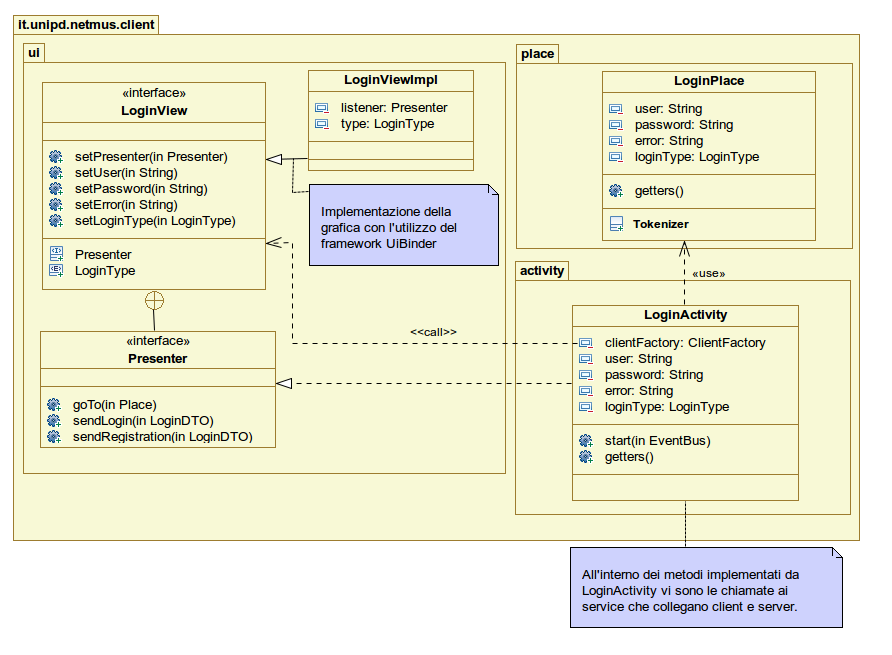
\includegraphics[width=14cm]{img/DP/package.png}
\caption{Diagramma \underline{UML}\ delle classi che descrive le dipendenze
fondamentali presenti all'interno del package client.}
\end{figure}

\subsection*{Requisiti obbligatori soddisfatti}
\begin{itemize}
	\item C1FN-1 Web Application NetMus
	\item C1QN-2.6 Manutenibilit\`a
\end{itemize}
\subsection*{Requisiti desiderabili e opzionali soddisfatti}
\begin{itemize}
    \item Nessuno.
\end{itemize}
\subsection*{Schema delle dipendenze architetturali}
Utilizzeremo le classi impegnate nelle procedure di autenticazione per spiegare
nel dettaglio le dipendenze presenti tra le componenti del package
\emph{client}. 
Queste dipendenze aderiscono al pattern MVP ed in particolare sono introdotte
dal framework MVP con Place e Activity.\\
Questo schema si ripete anche per gli altri gruppi funzionali di componenti:
profile e edit user.


Come possiamo vedere dal diagramma delle classi, la dichiarazione dei metodi
necessari alla comunicazione tra view e model viene fatta nell'interfaccia 
\co{Presenter} innestata nell'interfaccia \co{LoginView}. Cos\`i \co{LoginView}
si prende carico della definizione del presenter, anche se l'implementazione sta
nella classe \co{LoginActivity}, creando una forte dipendenza tra le componenti view e
presenter ma con il vantaggio di rimuovere qualsiasi tipo di collegamento
diretto dell'interfaccia grafica con il model.\\
La parte di visualizzazione vera e propria dei dati risiede in
\co{LoginViewImpl} che viene caricata con il deferred binding all'avvio
dell'applicazione garantendo buona separazione tra parte grafica e parte logica
e di conseguenza buona estendibilit\`a.\\
Questo schema di classi gestisce
anche la funzione di mantenimento dello stato lato client grazie a
\co{LoginPlace}. La classe Place mantiene alcune informazioni per definire lo
stato corrente e le rende disponibili, fornendo metodi \emph{get}, ad ogni
Activity che fa avviare. L'Activity a sua volta pu\`o inviarle, chiamando i
metodi \emph{set}, alla View che completa cos\`i il ciclo necessario al
mantenimento dello stato in ogni componente impiegata per la costruzione delle pagine.

\subsection*{Tipo, obiettivo e funzione del componente} % LASCIARE WARNING
Il package \emph{client} rappresenta la parte del sistema con la quale l'utente
pu\`o interagire. Tutte le sue classi ed i suoi sottopackage saranno compilati in
JavaScript da GWT, prima che il sistema venga depositato nel dominio
\emph{appspot.com} di Google. Contiene la classe \underline{Entry Point}
\co{NetMus}.
\subsection*{Attivit\`a svolte e dati trattati}
Le attivit\`a svolte dalle sue classi verranno qui di seguito descritte.

\subsection{Classe NetMus}
\subsubsection*{Requisiti obbligatori soddisfatti}
\begin{itemize}
	\item C1FN-1 Web Application NetMus
	\item C1VN-1.12 Deve utilizzare tecnologie GAE e GWT
\end{itemize}
\subsection*{Requisiti desiderabili e opzionali soddisfatti}
\begin{itemize}
  \item Nessuno.
\end{itemize}
\subsubsection*{Tipo, obiettivo e funzione del componente}
Questa classe rappresenta l'Entry Point di GWT che genera tutte le altre
componenti e rende disponibile e visibile l'intero sistema.\\
In particolare andr\`a a creare dinamicamente il \co{ClientFactoryImpl} adatto,
nel caso ce ne fossero diversi, e lo aggancia insieme all'EventBus al nostro
\co{NetmusPlaceHistoryMapper} ed al \co{NetmusActivityMapper}.
Inoltre allaccia al body Html il widget principale dell'applicazione.
\subsubsection*{Attivit\`a svolte e dati trattati}
\co{Netmus} praticamente si occupa di avviare il sistema e portare l'utente alla
pagina iniziale di Login o, se gi\`a autenticato, alla sua pagina Profilo.
\begin{longtable}{|p{0.4\textwidth}|p{0.4\textwidth}|}
\hline
\rowcolor{orange} \bo{Attributo} & \bo{Descrizione} \\
\hline
\endhead
\hline
\multicolumn{2}{|c|}{\textit{continua alla pagina successiva}}\\
\hline
\endfoot
\endlastfoot
- default\_place: Place &  Primo Place istanziato, avvia la
\co{LoginActivity}.\\\hline
- app\_widget: SimplePanel & Primo widget aggiunto al \co{RootPanel}
costituisce il corpo della pagina di login\\\hline
 - login\_service\_svc: LoginService Async & Inizializza l'interfaccia
 asincrona tramite Dynamic loading utilizzando il metodo \co{create()}
 per permettere la comunicazione \underline{RPC} con il server.\\\hline
\caption{Campi dati di Netmus}
\end{longtable}

\newpage
\begin{longtable}{|p{0.4\textwidth}|p{0.4\textwidth}|}
\hline
\rowcolor{orange} \bo{Metodo} & \bo{Descrizione} \\
\hline
\endhead
\hline
\multicolumn{2}{|c|}{\textit{continua alla pagina successiva}}\\
\hline
\endfoot
\endlastfoot
+ onModuleLoad() & \`E il metodo d'ingresso dell'applicazione, chiamato
automaticamente caricando un modulo che istanzia l'implementazione
dell'interfaccia EntryPoint .\\\hline
 + startNetmus() & Istanzia e inizializza i principali moduli
 dell'applicazione, quali \co{ClientFactory}, \co{ActivityMapper},
 \co{PlaceHistoryMapper} e \co{RootPanel}.\\\hline
\caption{Metodi di Netmus}
\end{longtable}


\subsection{Classe ClientFactoryImpl (\emph{Abstract Factory})}
\subsubsection*{Requisiti obbligatori soddisfatti}
\begin{itemize}
    \item C1FN-1 Web Application NetMus
    \item C1QO-2.1 Accessibilit\`a
    \item C1QN-2.3 Portabilit\`a
    \item C1QN-2.6 Manutenibilit\`a
\end{itemize}
\subsubsection*{Requisiti desiderabili e opzionali soddisfatti}
\begin{itemize}
	\item Nessuno
\end{itemize}
\subsubsection*{Tipo, obiettivo e funzione del componente}
In NetMus \`e disponibile un'unica implementazione dell'interfaccia
\co{ClientFactory}, poich\'e per il momento la portabilit\`a richiesta per i
principali browser in circolazione \`e gi\`a soddisfatta e non verranno
implementate interfacce alternative. Nella classe si definiscono
le propriet\`a di un vista (desktop) del sistema.
\subsubsection*{Attivit\`a svolte e dati trattati}
La classe si occupa di istanziare l'event bus, il place controller e le varie
view. L'event bus gestisce le comunicazioni tra componenti, il place
controller permette la navigazione tra i Place e si occupa di avvisare
l'utente prima del passaggio ad uno stato differente.
\begin{longtable}{|p{0.4\textwidth}|p{0.4\textwidth}|}
\hline
\rowcolor{orange} \bo{Attributo} & \bo{Descrizione} \\
\hline
\endhead
\hline
\multicolumn{2}{|c|}{\textit{continua alla pagina successiva}}\\
\hline
\endfoot
\endlastfoot
- event\_bus: EventBus \emph{static final} & Gestore del flusso degli
eventi.\\\hline
- place\_controller: PlaceController \emph{static final} & Classe del
\underline{framework} GWT Activity and Place che gestisce automaticamente i
Place.\\\hline - login\_view: LoginView \emph{static final} & Interfaccia
pubblica di Login.\\\hline - profile\_view: ProfileView \emph{static final} &  Interfaccia pubblica di
Login.\\\hline 
\caption{Campi dati di ClientFactoryImpl}
\end{longtable}
\begin{longtable}{|p{0.4\textwidth}|p{0.4\textwidth}|}
\hline
\rowcolor{orange} \bo{Metodo} & \bo{Descrizione} \\
\hline
\endhead
\hline
\multicolumn{2}{|c|}{\textit{continua alla pagina successiva}}\\
\hline
\endfoot
\endlastfoot
+ getters() & Tutti gli attributi privati di questa
classe hanno i relativi metodi \emph{get}.\\\hline 
\caption{Metodi di ClientFactoryImpl}
\end{longtable}



\newpage
\section{Package client.ui} % LASCIARE WARNING
\subsection*{Requisiti obbligatori soddisfatti}
\begin{itemize}
	\item C1FN-1 Web Application NetMus
	\item C1FN-1.1 Grafica simile ad \underline{iTunes}
	\item C1QN-2.3 Portabilit\`a
	\item C1QN-2 Utilizzo
\end{itemize}
\subsection*{Requisiti desiderabili e opzionali soddisfatti}
\begin{itemize}
    \item C1QD-1.6.1 Scalabilit\`a interfaccia grafica
    \item C1QD-2.4 Supporto multi-lingua
    \item C1QO-2.1 Accessibilit\`a
\end{itemize}
\subsection*{Tipo, obiettivo e funzione del componente}
Il package \emph{ui} contiene le interfacce e le implementazioni delle View del
sistema. Le View generano gli ambienti grafici (assimilabili all'interfaccia
utente di iTunes) con cui gli utenti possono interagire e si occupano di
catturare gli eventi da essi prodotti. \\
L'implementazione della grafica sar\`a eseguita con l'utilizzo del framework
UiBinder ed il conseguente utilizzo del linguaggio CSS3 per la formattazione
che garantir\`a dei buoni livelli di accessibilit\`a.
Le annotazioni utilizzate all'interno del codice Java per interagire con i file
xml previsti da UiBinder saranno:
\begin{itemize}
  \item \bo{@UiField}: gli attributi marcati in questo modo hanno lo stesso nome
  di un elemento del file .xml a cui possono accedere successivamente alla
  chiamata \emph{uiBinder.createAndBindUi (this)} che associa all'attributo
  \underline{Java} l'istanza appropriata di \co{SpanElement}. Questi attributi
  avranno visibilit\`a \emph{package}.
  \item \bo{@UiHandler(``name\_of\_uifield'')}: permette di scrivere dei metodi
  che gestiscono gli eventi scatenati dal parametro UiField senza
  dover dichiarare le classi handler previste da Java.
\end{itemize}
\subsection*{Attivit\`a svolte e dati trattati}
In sostanza svolge il compito di organizzare le informazioni del model in un
interfaccia accessibile dall'utente.


\subsection{Interfaccia LoginView / Classe LoginViewImpl}
\subsubsection*{Requisiti obbligatori soddisfatti}
\begin{itemize}
    \item C1FN-1.1 Grafica simile ad iTunes
	\item C1FN-1.2 Registrazione
	\item C1QN-2 Utilizzo
	\item C1QN-2.3 Portabilit\`a
	\item C1VN-2.5 Semplicit\`a di utilizzo
\end{itemize}
\subsection*{Requisiti desiderabili e opzionali soddisfatti}
\begin{itemize}
    \item C1QD-1.6.1 Scalabilit\`a interfaccia grafica
    \item C1FO-1.2.1 Pagina login indipendente
    \item C1QO-2.1 Accessibilit\`a
\end{itemize}
\subsubsection*{Tipo, obiettivo e funzione del componente}
La classe \co{LoginView} rappresenta la finestra di login fornita all'utente
ogni qualvolta questo accede al sistema senza essersi gi\`a autenticato
precedentemente. \`E possibile effettuare la registrazione a NetMus
selezionando l'apposita sezione ed inserendo un nuovo username ed una password
con le relative conferme. La classe \co{LoginViewImpl} implementa l'interfaccia
\co{LoginView} che estende \co{isWidget} (interfaccia introdotta da GWT 2.1)
permettendo l'utilizzo di UiBinder per la disposizione dei widget e la gestione
degli handler. \\
Le azioni invocabili
sono tutte definite nell'interfaccia interna
\co{Presenter} e saranno utilizzate all'interno dei metodi handler. Viene
definito un \emph{enum} riguardante la tipologia di login che viene utilizzato
anche da \co{LoginActivity} e \co{LoginPlace}. \\ I contratti dei metodi (che vengono
implementati in \co{LoginActivity}) e l'\emph{enum} in questione sono:
\begin{itemize}
  \item public void goTo(in Place) : permette di spostarsi in un
  place differente anche relativo ad un'altra view. Ad esempio per aprire la pagina di
  \co{ProfileView} una volta verificato il login.
  \item public void sendLogin(in String, in String) throws  LoginException
  : invia al server i dati di login inseriti
  dall'utente. Viene inviata la richiesta di verifica del login con i dati
  presenti nel Datastore tramite una \underline{chiamata asincrona} ad un metodo
  di \co{LoginService}. La chiamata RPC pu\`o lanciare eventi di tipo
  \co{LoginException}.
  \item public void sendGoogleLogin(in String, in String)
  throws LoginException : apre una pagina del sistema che richiama la servlet
  \co{LoginGoogleServlet}.
  \item public void sendRegistration(in String, in String, in String)
  throws RegistrationException : invia al server i dati di registrazione inseriti
  dall'utente. Viene fatto un primo controllo sulla validit\`a dei dati e de
  positivo viene inviata la richiesta di inserimento dell'utente nel database
  tramite una chiamata asincrona ad un metodo di \co{LoginService}. La chiamata
  RPC pu\`o lanciare eventi di tipo \co{RegistrationException}.
  \item public enum LoginType \{NETMUSLOGIN, NETMUSREGISTRATION,
  GOOGLELOGIN\} : Definisce le tipologie di login e registrazione possibili.
\end{itemize}
\subsubsection*{Attivit\`a svolte e dati trattati} La classe permette all'utente
di scegliere se effettuare il login tramite NetMus o Google oppure la
registrazione attraverso un'interfaccia grafica accattivante e di semplice utilizzo, contiene una form
per l'inserimento password e nome utente e pu\`o visualizzare warning se i dati
inseriti non sono corretti. \\
La pagina \`e disponibile in due lingue: italiano ed inglese.\\
Tra gli attributi ed i metodi presentati vi sono anche i widget e gli handler
implementati con UiBinder in LoginViewImpl.
\begin{longtable}{|p{0.4\textwidth}|p{0.4\textwidth}|}
\hline
\rowcolor{orange} \bo{Attributo} & \bo{Descrizione} \\
\hline
\endhead
\hline
\multicolumn{2}{|c|}{\textit{continua alla pagina successiva}}\\
\hline
\endfoot
\endlastfoot
+ myConstants: MyConstants & Gestore dell'internazionalizzazione associato a
questa pagina.\\\hline 
- listener: Presenter & Presenter associato a questa
pagina.\\\hline 
- type: LoginType & Tipologia di accesso che si sta effettuando.\\\hline
@UiField container: HTMLPanel & Finestra che contiene l'intera pagina.\\\hline
@UiField login: Label & Etichetta che se cliccata invia i dati e avvia
la procedura di login o di registrazione.\\\hline 
@UiField register: Label & Etichetta che se cliccata apre la
visualizzazione del form di registrazione.\\\hline 
@UiField account: Label &
Etichetta che descrive i campi di inserimento login e password.\\\hline
@UiField user: TextBox & Campo per l'inserimento del login.\\\hline
@UiField password: TextBox & Campo per l'inserimento della password.\\\hline
@UiField c\_password: TextBox & Campo per l'inserimento della
password di conferma.\\\hline 
@UiField error: Label & Etichetta che contiene il testo di eventuali
errori avvenuti durante il login o la registrazione.\\\hline 
@UiField check\_google: RadioButton & Bottone di selezione del tipo di
login.\\\hline 
@UiField check\_netmus: RadioButton & Bottone di selezione del tipo di
login.\\\hline
\caption{Campi dati di LoginView}
\end{longtable}
\begin{longtable}{|p{0.4\textwidth}|p{0.4\textwidth}|}
\hline
\rowcolor{orange} \bo{Metodo} & \bo{Descrizione} \\
\hline
\endhead
\hline
\multicolumn{2}{|c|}{\textit{continua alla pagina successiva}}\\
\hline
\endfoot
\endlastfoot
+ setPresenter(in Presenter) & Questo metodo viene usato da
\co{LoginActivity} per impostare una sua istanza come implementazione
del presenter di \co{LoginView}.\\\hline 
+ setUser(in String) & Questo metodo viene usato da
\co{LoginActivity} per impostare l'username inserito nel precedente
tentativo di login o registrazione.\\\hline 
+ setPassword(in String) & Questo metodo viene usato da
\co{LoginActivity} per impostare la password inserita nel precedente
tentativo di login o registrazione.\\\hline 
+ setError(in String) & Questo metodo viene usato da
\co{LoginActivity} per impostare il testo di un errore occorso nel
precedente tentativo di login o registrazione.\\\hline
+ setLoginType(in LoginType) & Serve ad impostare il tipo di login o
registrazione che si sta effettuando.\\\hline 
+ setLayout() & Aggiunta il layout all'avvio.\\\hline
@UiHandler(``login'') handleClickLogin(in ClickEvent) & Quando viene
premuto il bottone di login invia all'activity associata la richiesta di login o
registrazione.\\\hline @UiHandler(value=\{``user'', ``password'', ``c\_password''\})
handlePressEnterPassword(in KeyPressEvent) & Quando viene premuto in tasto
``enter'' invia all'activity associata la richiesta di login o
registrazione.\\\hline @UiHandler(``register'') handleClickRegister(in ClickEvent) & Se la pagina si
trova nello stato \co{LoginType.LOGINNETMUS} ridispone gli elementi in
modo da visualizzare il form intero per la registrazione, altrimenti
nasconde i campi per registrazione lasciando solamente quelli per il
login.\\\hline
@UiHandler(``check\_google'') handleClickGoogle(in ClickEvent) & Viene
avviato quando l'utente seleziona Google come tipologia di login e
aggiorna l'attributo \co{type}. \\\hline @UiHandler(``check\_netmus'')
handleClickNetmus(in ClickEvent) & Viene
avviato quando l'utente seleziona NetMus come tipologia di login e
aggiorna l'attributo \co{type}.\\\hline
\caption{Metodi di LoginView}
\end{longtable}

\subsection{Interfaccia ProfileView / Classe ProfileViewImpl}
\subsubsection*{Requisiti obbligatori soddisfatti}
\begin{itemize}
    \item C1FN-1.1 Grafica simile ad iTunes
	\item C1FN-1.1.1 Brani elencati opportunamente
	\item C1FN-1.1.2 Menu laterali
	\item C1FN-1.1.3 Visualiz. info dettagliate dei brani
    \item C1FN-1.4 Gestione profilo personale
    \item C1FN-1.4.1 Modifica informazioni personali
    \item C1FN-1.4.2 Cambio password
    \item C1FN-1.4.3 Cancellazione del proprio account
    \item C1QN-2 Utilizzo
    \item C1QN-2.3 Portabilit\`a
    \item C1VN-2.5 Semplicit\`a di utilizzo
\end{itemize}
\subsection*{Requisiti desiderabili e opzionali soddisfatti}
\begin{itemize}
    \item C1FD-1.1.4 Visualizza player YouTube
    \item C1FD-1.3 Personalizzazione del catalogo 
    \item C1FD-1.3.1 Cancellazione brano
    \item C1FO-1.3.3 Creazione playlist  
    \item C1FO-1.3.4 Ranking brani  
    \item C1FD-1.4.4 Pubblicazione
    \item C1FD-1.5 Riproduzione tracce in streaming
    \item C1QD-1.6.1 Scalabilit\`a interfaccia grafica
    \item C1FD-1.7 Interazione con altri utenti
    \item C1FD-1.7.1 Visualizzazione altri profili
    \item C1FO-1.8.1 Esportazione \underline{PDF}
    \item C1QO-2.1 Accessibilit\`a
\end{itemize}
\subsubsection*{Dettaglio del riempimento di ProfileView all'avvio di una nuova
ProfileActivity}
\begin{figure}[h]
  \centering
  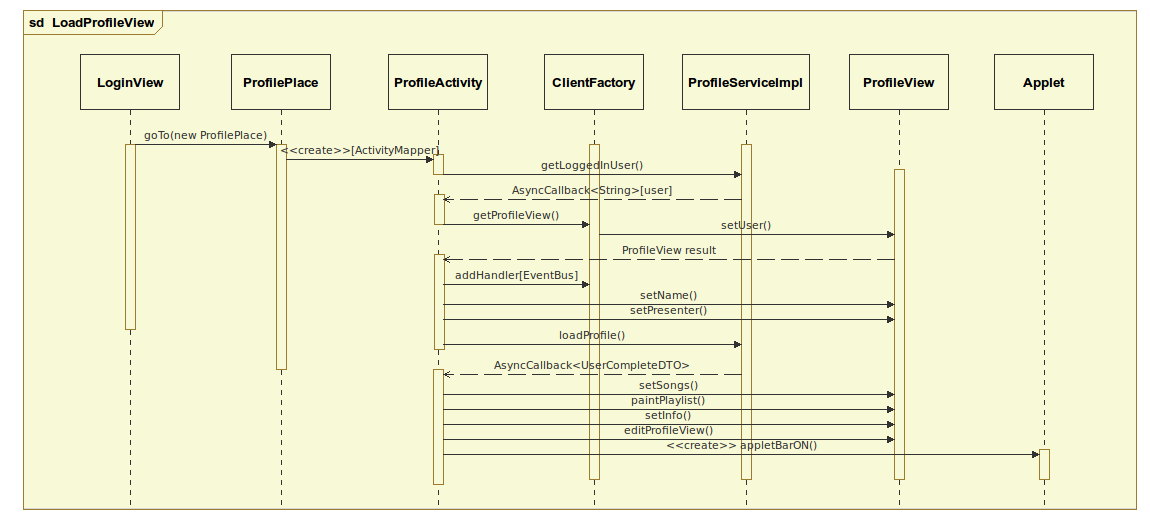
\includegraphics[width=15cm]{img/DP/loadProfileView.png}
\caption{Diagramma UML di sequnza che descrive nel dettaglio come viede
disegnata la ProfileView all'avvio di una nuova ProfileActivity}
%DESCRIZIONE DEL DIAGRAMMA.. ..  .  . . . . 
\end{figure}
\subsubsection*{Tipo, obiettivo e funzione del componente}
Il sistema mette a disposizione una vista per la visualizzazione del profilo e
dei brani di un generico utente registrato e per la riproduzione dalla musica
tramite un player streaming. La classe \co{ProfileViewImpl} implementa
l'interfaccia \co{ProfileView} che estende \co{isWidget} (interfaccia introdotta
da GWT 2.1). \\
Le azioni invocabili dai metodi handler sono tutte definite nell'interfaccia
interna \co{Presenter} ma l'implementazione risieder\`a in \co{ProfileActivity}
e comprender\`a chiamate asincrone al server attraverso i metodi di
\co{LoginService}, \co{LibraryService}, \co{SongsService} e \co{UsersService}.\\
I metodi in questione sono:
\begin{itemize}
    \item void logout(): effettua la deautenticazione dell'utente chiudendo la
    sessione HTTP corrente e rimuovendo il cookie relativo. Una volta effettuate
    queste operazioni viene aperta la pagina di \co{LoginView}.
    \item void goTo(Place place) : permette di spostarsi in un place differente
    anche relativo ad un'altra view. Ad esempio per aprire la pagina di
    \co{LoginView} dopo aver effettuato il logout.
    \item void editProfileView(String user): ricerca ed imposta i dati 
    dell'utente per poterli visionare ed eventualmente identificare.
    \item void setPlaylistList(): imposta la lista dei
    titoli delle singole playlist dell'utente create precedentemente.
    \item void setFriendList(): imposta la lista degli
    utenti affini su NetMus all'utente impostato precedentemente.
    \item void setSongInfo(): imposta il titolo della canzone in
    ascolto.
    \item void setPlaylistSongs(String titoloPlaylist): imposta le canzoni
    con i relativi album dato il nome di una playlist in input.
    \item void setSongs(): fornisce tutte le canzoni legate alla libraria
    musicale dell'utente attraverso una lista contenente gruppi di stringhe
    ordinate.
    \item void playYouTube(): dopo aver effettuato una ricerca su YouTube grazie
    alle classi del package \emph{server.youtube} fornisce il link youtube della
    canzone selezionata.
    \item void addPlaylist(String title): crea una nuova playlist a
    disposizione dell'utente che sta visualizzando la propria pagina.
    \item void addToPLaylist(String playlist, String autore, String titolo,
    String album): aggiunge la canzone in input alla playlist desiderata.
    \item void removeFromPLaylist(String playlist, String autore, String titolo,
    String album): rimuove la canzone in input dalla playlist desiderata.
    \item double setRating(String artist, String title, String album): fornisce
    il rating personale relativo ad una canzone e restituisce un valore double
    che rappresenta il rating globale di tutti gli utenti su quella canzone.
    \item void setSongFields(String autore, String titolo, String album):
    Imposta i campi che mostrano le informazioni relative al brano selezionato.
    \item void rateSong(String artist, String title, String album, int rate):
    attribuisce un punteggio compreso tra uno e cinque alla canzone selezionata.
    \item void deletePlaylist(String playlist): elimina la playlist
    indicata.
    \item void moveDownInPlaylist(String playlist, String autore, String
    titolo, String album): sposta in basso di una posizione la canzone della
    playlist selezionata.
    \item void moveUpInPLaylist(String playlist, String autore, String titolo,
    String album): sposta in alto di una posizione la canzone della playlist.
    \item
    void viewOtherLibrary(String user): controlla i permessi ed avvia la
    visualizzazione del profilo utente in input.
    \item void deleteSong(String autore, String titolo, String album): elimina
    dalla libreria dell'utente la canzone indicata.
    \item void exportPDF(String user): esporta la lista delle canzoni
    dell'utente in PDF.
    \item void editProfile(String user, String nickname, String firstname,
    String gender, String nationality, String aboutme, String Password):
    salva e aggiorna i dati dell'utente.
    \item editSongTitle(String newtitle, String oldtitle, String artist, String
    album): salva il titolo modificato della canzone.
    \item editSongAlbum(String newalbum, String oldalbum, String artist, String
    title): salva il nome dell'album modificato della canzone.
    \item void editSongArtist(String newartist, String oldartist, String title,
    String album): salva il nome dell'artista modificato.
\end{itemize}
\subsubsection*{Attivit\`a svolte e dati trattati}
Contiene il catalogo dei brani dell'utente attraverso il quale \`e possibile
visualizzare tutte le informazioni relative ad un brano e ordinare gli stessi
all'interno di comode playlist. Consente la creazione, la gestione e la
rimozione delle playlist in cui possono essere contenuti i brani. Attraverso una semplice
interfaccia permette di visualizzare lo streaming tramite il servizio di YouTube
dei brani o delle playlist selezionate. Contiene la lista dei profili che
l'utente pu\`o visualizzare e gli strumenti per navigare tra i cataloghi
musicali degli altri utenti. Permette inoltre di esportare la propria libreria
in formato PDF e di visualizzare molteplici statistiche riguardanti il catalogo
musicale. Consente infine di gestire, aggiornare od eliminare i dati del proprio
account.
\subsubsection*{Classi Interne} Viene implementata la classe interna \co{Song} la quale estende la classe astratta \co{Song} derivata da, e definita in, ProfileView. Lo scopo di questa classe \`e quello di rappresentare un oggetto che contenga al suo interno \emph{titolo}, \emph{autore} e \emph{album} di ciascun brano del catalogo. Questo risulta molto utile anche nella gestione di molte Widget GWT predisposte per elaborare in input liste di oggetti \emph{List\textless Type\textgreater}. Viene inoltre ridefinito il metodo \emph{equals(Song)} il quale consente di confrontare l'uguaglianza di due brani in base ai loro attributi.
\subsubsection*{Interfacce Interne}
All'interno di \co{ProfileViewImpl} vengono definite due interfacce,
rispettivamente \emph{MyCellTableResources} e
\emph{MyCellTableResourcesPlaylist }, le quali estendono entrambe
\emph{CellTable.Resources}. Al loro interno vengono ridefinite le
caratteristiche del layout a loro associate e in particolar modo i file di stile
CSS a cui devono far riferimento. Una volta istanziate come classe
tramite il metodo \emph{GWT.create()} vengono assegnate come modello di stile
alle istanze di widget \emph{CellTable} per poterne definirne le caratteristiche
estetiche tramite i fogli di stile precedentemente impostati.
\\
\begin{longtable}{|p{0.4\textwidth}|p{0.4\textwidth}|}
\hline
\rowcolor{orange} \bo{Attributo} & \bo{Descrizione} \\
\hline
\endhead
\hline
\multicolumn{2}{|c|}{\textit{continua alla pagina successiva}}\\
\hline
\endfoot
\endlastfoot
+ myConstants: MyConstants & Gestore dell'internazionalizzazione associato a
questa pagina.\\\hline 
- listener: Presenter & Riferimento all'istanza di ProfileActivity che
implementa l'interfaccia Presenter definita in ProfileView.\\\hline
- name: String & Il nome dell'account dell'utente.\\\hline
- vertical\_offset: int \emph{default = 65} & Spazio in pixel tra
l'interfaccia principale e il margine inferiore della finestra del
browser.\\\hline
- vertical\_semioffset: int \emph{default = 275} & Spazio in pixel tra
il margine inferiore della sezione centrale dell'interfaccia grafica e
il margine inferiore della finestra del browser.\\\hline
- rating: int & Il rating personale dell'utente rispetto ad un brano.\\\hline
- global\_rating: double & Il rating globale su netmus rispetto ad un
brano.\\\hline
- password: String & la nuova password inserita dall'utente.\\\hline
- cpassword: String & la conferma della nuova password inserita
dall'utente.\\\hline
- song\_list: CellTable\textless Song\textgreater & la widget a tabella che
rappresenta il catalogo dei brani dell'utente.\\\hline;
- rm\_link: HandlerRegistration & Registratore dell'handler su
l'indirizzo link del player youtube.\\\hline
- rm\_fw: HandlerRegistration & Registratore dell'handler sul bottone di forward
dei comandi di streaming.\\\hline
- rm\_rw: HandlerRegistration & Registratore dell'handler sul bottone di rewind
dei comandi di streaming.\\\hline
@UiField logout: Anchor & Link per il logout.\\\hline
@UiField user: Label & Etichetta che visualizza il nome dell'utente.\\\hline
@UiField num\_song: Label & Etichetta che rappresenta il numero di
brani a catalogo.\\\hline
@UiField playlist\_title: Label & Etichetta che rappresenta il titolo
dell'elenco delle playlist.\\\hline
@UiField track\_title: Label & Etichetta che rappresenta il titolo della
canzone visualizzata nelle informazioni dettagliate.\\\hline
@UiField info\_youtube\_link: Label & Etichetta che mostra l'indirizzo
d'origine del video youtube in riproduzione.\\\hline
@UiField insert\_song: Label & Etichetta che visualizza in verde il
titolo selezionato a catalogo e che risulta possibile inserire nella
playlist aperta.\\\hline
@UiField remove\_song: Label & Etichetta che visualizza in rosso il
titolo selezionato nella playlist e che pu\`o essere rimosso.\\\hline
@UiField song\_title: Label & Etichetta che mostra il titolo della
canzone nelle informazioni dettagliate.\\\hline
@UiField song\_artist: Label & Etichetta che mostra l'autore della
canzone nelle informazioni dettagliate.\\\hline
@UiField song\_album: Label & Etichetta che mostra il titolo dell'album
della canzone nelle informazioni dettagliate.\\\hline
@UiField song\_genre: Label & Etichetta che mostra il genere della
canzone nelle informazioni dettagliate.\\\hline
@UiField song\_year: Label & Etichetta che mostra l'anno della canzone
nelle informazioni dettagliate.\\\hline
@UiField song\_composer: Label & Etichetta che mostra il genere della
canzone nelle informazioni dettagliate.\\\hline
@UiField song\_track: Label & Etichetta che mostra il numero di
traccia della canzone nelle informazioni dettagliate.\\\hline
@UiField edit\_profile\_password: Label & Etichetta 
password nella finestra dell'account.\\\hline
@UiField edit\_profile\_cpassword: Label & Etichetta 
conferma password nella finestra dell'account.\\\hline
@UiField edit\_profile\_nickname: Label & Etichetta nickname
dell'utente nella finestra dell'account.\\\hline
@UiField edit\_profile\_name: Label & Etichetta  nome
dell'utente nella finestra dell'account.\\\hline
@UiField edit\_profile\_surname: Label & Etichetta cognome
dell'utente nella finestra account.\\\hline
@UiField edit\_profile\_nationality: Label & Etichetta 
nazione dell'utente nella finestra dell'account.\\\hline
@UiField edit\_profile\_gender: Label & Etichetta il sesso
dell'utente nella finestra dell'account.\\\hline
@UiField edit\_profile\_labelCpassword: Label & Etichetta conferma
password nella finestra dell'account.\\\hline
@UiField stat\_tracks: Label & Etichetta che indica il numero di brani
nella finestra delle statistiche\\\hline @UiField : Label & \\\hline
@UiField stat\_preferred: Label & Etichetta che indica l'autore
preferito all'interno della finestra delle statistiche\\\hline
@UiField stat\_preferreds: Label & Etichetta che indica la canzone
preferita all'interno della finestra delle statistiche\\\hline
@UiField stat\_preferredn: Label & Etichetta nella finestra delle statistiche
che rappresenta la canzone preferita dall'intera utenza di Netmus\\\hline
@UiField info\_text: Label & Etichetta che rappresenta il brano in
esecuzione nella finestra informativa della view\\\hline
@UiField catalogo: CellTable\textless Song\textgreater & Tabella che
mostra l'intero catalogo dell'utente.\\\hline
@UiField catalogo\_container: HTMLPanel & Elemento che definisce l'area
dove viene inserito e visualizzato il catalogo delle canzoni.\\\hline
@UiField playlist\_container: HTMLPanel & Elemento che definisce l'area
dove viene inserita la lista di canzoni di una playlist.\\\hline
@UiField playlist\_contenuto: HTMLPanel & Inserita all'interno di
playlist\_container contiene la tabella che visualizza il contenuto di
una playlist.\\\hline
@UiField playlist\_songs: HTMLPanel & Elemento all'interno di
playlist\_container dove viene inserita la CellTable con i dati delle
canzoni della playlist.\\\hline
@UiField song\_container: HTMLPanel & Elemento che definisce l'area dove
vine inerito il dettaglio di una canzone.\\\hline
@UiField song\_contenuto: HTMLPanel & Elemento inserito all'interno di
song\_container che contiene i campi dati sui dettagli della canzone.\\\hline
@UiField main\_panel: HTMLPanel & Elemento principale dell'interfaccia
grafica, situato a destra rappresenta la parte principale dell'intero
\underline{UI}.\\\hline @UiField left\_panel: HTMLPanel & Secondo elemento
principale della UI, rappresenta l'intera zona che contiene i menu sulla sinistra.\\\hline
@UiField playlists: HTMLPanel & Elemento inserito all'interno di
left\_panel che contiene l'elenco delle playlist dell'utente.\\\hline
@UiField friends: HTMLPanel & Elemento inserito all'interno di
left\_panel che contiene l'elenco degli amici su netmus.\\\hline
@UiField friends\_titolo: HTMLPanel & Elemento che contiene il titolo
dell'area in cui compare la lista degli amici su netmus.\\\hline
@UiField info: HTMLPanel & Elemento che contiene le informazioni
relative al brano riprodotto.\\\hline
@UiField search: HTMLPanel & elemento che contiene l'input di ricerca
nel catalogo.\\\hline
@UiField youtube: HTMLPanel & Elemento che contiene il tasto player di
youtube e il player stesso all'occorrenza.\\\hline
@UiField classifica: HTMLPanel & Elemento che contiene le stelle per la
votazione ed il rating personale.\\\hline
@UiField info\_youtube: HTMLPanel & Elemento che contiene le informazioni
riguardanti il brano che sta venendo riprodotto nel player youtube.\\\hline
@UiField youtube\_appendice: HTMLPanel & Elemento che contiene il tasto
x chiudere il player youtube.\\\hline
@UiField edit\_profile: HTMLPanel & Elemento che rappresenta la finestra
a scomparsa che contiene le informazioni sull'account.\\\hline
@UiField edit\_profile\_aboutme: HTMLPanel & Elemento che contiene i
dati personali scritti dall'utente all'interno della finestra
dell'account.\\\hline
@UiField covers\_container: HTMLPanel & Elemento che rappresenta l'area in cui
vengono caricate le copertine del cover mode. \\\hline
@UiField popup: HTMLPanel & Rappresenta la finestra di popup con conferma che
propone errori e messaggi. \\\hline
@UiField popup\_fast: HTMLPanel & Rappresenta la finestra di popup senza
conferma che propone errori e messggi. \\\hline
@UiField statistics: HTMLPanel & Rappresenta la finestra in cui compaiono le
statistiche. \\\hline

@UiField play: Image & Rappresenta il bottone play/pause
dell'interfaccia principale.\\\hline
@UiField play\_youtube: Image & Rappresenta il bottone play nell'area del
youtube player.\\\hline
@UiField forward: Image & Rappresenta il tasto forward dell'interfaccia
principale.\\\hline
@UiField rewind: Image & Rappresenta il tasto rewind dell'interfaccia
principale.\\\hline
@UiField cover: Image & Inserito in panel\_left; rappresenta la cover della
canzone in play sul player youtube.\\\hline
@UiField edit\_button: Image & Rappresenta il bottone d'accesso alle
informazioni della canzone selezionata.\\\hline
@UiField account\_button: Image & Rappresenta il bottone d'accesso ai
dati dell'utente.\\\hline
@UiField social\_button: Image & Rappresenta il bottone d'accesso alle
funzionalit\`a social di netmus\\\hline
@UiField star1/star2/star3/star4/star5: Image & Rappresentano le stelle
per il voto personale sulla canzone.\\\hline
@UiField starG1/starG2/starG3/starG4/starG5: Image & Rappresentano le
stelle del voto globale su di una canzone.\\\hline
@UiField chiudi\_playlist: Image & Rappresenta il bottone per chiudere la
playlist.\\\hline @UiField chiudi\_song: Image & Rappresenta il bottone
per chiudere il dettaglio di una canzone.\\\hline
@UiField logo\_youtube: Image & Rappresenta l'immagine del logo di
YouTube.\\\hline
@UiField chiudi\_youtube: Image & Rappresenta il bottone per chiudere il
player di YouTube.\\\hline
@UiField aggiungi\_branoplaylist: Image & Rappresenta il bottone per
aggiungere un brano selezionato nella playlist aperta\\\hline
@UiField rimuovi\_branoplaylist: Image & Rappresenta il bottone per
rimuovere dalla playlist il brano selezionato.\\\hline
@UiField song\_cover: Image & Rappresenta l'immagine della copertina
dell'album del brano selezionato nelle informazioni dettagliate di un
brano.\\\hline
@UiField elimina\_playlist: Image & Rappresenta il bottone per eliminare
definitivamente una playlist.\\\hline
@UiField elimina\_song: Image & Rappresenta il bottone per eliminare
definitivamente una canzone dal proprio catalogo. \\\hline
@UiField edit\_profile\_chiudi: Image & Rappresenta il bottone per
chiudere la finestra delle informazioni sull'account.\\\hline
@UiField edit\_profile\_checkImg: Image & Rappresenta l'immagine di
conferma per il salvataggio dei dati all'interno della finestra per
gestire le informazioni sull'account.\\\hline
@UiField switch\_cover: Image & Rappresenta il bottone per entrare in cover
mode. \\\hline
@UiField switch\_list: Image & Rappresenta il bottone per visulaizzare il
catalogo come una lista. \\\hline
@UiField loading: Image & Rappresenta la scritta che compare durante i
caricamenti. \\\hline
@UiField pdf: Image & Rappresenta l'icona x l'esportazione del catalogo.
\\\hline
@UiField statistics\_open: Image & Rappresenta l'immagine per aprire la finestra
delle statistiche. \\\hline
@UiField edit\_profile\_clear: Image & Rappresenta il bottone all'interno dell
popup edit profile per eliminare l'account.\\\hline
@UiField flag\_ita: Image & Rappresenta la bandiera per impostare la lingua
italiana. \\\hline
@UiField flag\_eng: Image & Rappresenta la bandiera per impostare la lingua
inglese. \\\hline
@UiField up: Image & Rappresenta la freccia per l'ordinamento brani nella
playlist. \\\hline
@UiField down: Image & Rappresenta la freccia per l'ordinamento brani nella
playlist. \\\hline

@UiField edit\_profile\_check: Button & Rappresenta il bottone per il
salvataggio dei dati personali all'interno della finestra informazioni
dell'account.\\\hline
@UiField edit\_profile\_vc: VerticalPanel & Rappresenta una componente di layout
spaziale per la finestra informazioni dell'account.\\\hline
@UiField : TextBox & Rappresenta il campo di input in cui inserire i
termini per la ricerca nel catalogo.\\\hline
- playlist\_opened: boolean & Rappresenta se il pannello con il contenuto di una
playlist risulta aperto o meno. \\\hline
- song\_opened: boolean & Rappresenta se il pannello con il contenuto dei
dettagli di una canzone risulta aperto o meno. \\\hline
- youtube\_status: int & Rappresenta lo stato del player youtube. 0: fermo, 1:
in play, -1: in pausa, 2/3: in play con una canzone differente selezionata nel
catalogo. \\\hline
- last\_selected: int & Rappresenta la selezione dell'utente relativamente al
catalogo o ad una playlist. 0: viene selezionato un brano sul catalogo, 1: viene
selezionato un brano nella playlist. \\\hline
- playing: intn & Rappresenta se \`e in riproduzione un brano contenuto in una
playlist o nel catalogo. 0: catalogo, 1: playlist. \\\hline
- selected\_song: Song & Rappresenta la canzone selezionata dall'utente sul
catalogo. \\\hline
- selected\_song\_playlist: Song & Rappresenta la canzone selezionata
dall'utente nella playlist.\\\hline
- played\_song: Song & Rappresenta la canzone in riproduzione\\\hline
@UiField selected\_album: String &  Rappresenta l'album selezionato
dall'utente\\\hline
- canzoni\_catalogo: List\textless Song\textgreater & Rappresenta le
canzoni caricate a catalogo.\\\hline
- canzoni\_playlist : List\textless Song\textgreater & Rappresenta le
canzoni caricate nella playlist aperta.\\\hline - dataProvider\_playlist:
ListDataProvider\textless Song\textgreater & Rappresenta le canzoni
visualizzate nella CellTable del catalogo\\\hline - dataProvider\_catalogo:
ListDataProvider\textless Song\textgreater & Rappresenta le canzoni visualizzate
dalla CellTable nella playlist.\\\hline
ListDataProvider\textless Song\textgreater dataProvider\_album & Rappresenta la
lista delle canzoni di un album quando caricato\\\hline
\caption{Campi dati di ProfileView}
\end{longtable}
\begin{longtable}{|p{0.4\textwidth}|p{0.4\textwidth}|}
\hline
\rowcolor{orange} \bo{Metodo} & \bo{Descrizione} \\
\hline
\endhead
\hline
\multicolumn{2}{|c|}{\textit{continua alla pagina successiva}}\\
\hline
\endfoot
\endlastfoot
+ setPresenter(in Presenter) & Questo metodo viene usato da
\co{ProfileActivity} per impostare una sua istanza come implementazione
del presenter di \co{ProfileView}.\\\hline 
+ setName(in String): & Questo metodo viene usato da
\co{ProfileActivity} per fornire il nome del profilo alla creazione della
\co{ProfileView}. \\\hline 
+ setNumeroBrani(in int) & Questo metodo viene usato da
\co{ProfileActivity} per fornire il numero di brani alla creazione della
\co{ProfileView}.\\\hline 
+ setUser(in String) & Questo metodo viene usato da
\co{ProfileActivity} per fornire l'\underline{username} dell'utente alla
creazione della \co{ProfileView}.\\\hline
+ paintCatalogo(in List\textless String\textgreater) & Riempie il
catalogo\\\hline 
+ paintPlaylist(in String[]) & Riempie la lista delle playlist.\\\hline
+ paintPlaylistSongs(List\textless String\textgreater) &
Riempie la singola playlist delle sue canzoni.\\\hline 
+ paintFriendlist(in String[]) & Riempie la lista dei contatti.\\\hline
+ setInfo(in String) & Imposta la finestra informativa.\\\hline
+ viewPlaylist(in String) & Visualizza la playlist scelta.\\\hline
+ closePlaylist() & Chiude il gestore della playlist.\\\hline
+ playYouTube(in String) & Apre il player youtube sulla relativa
canzone.\\\hline 
+ closeYouTube() & Chiude il player youtube.\\\hline
+ setBranoCatalogo(in Song) & Imposta il brano selezionato sul catalogo.\\\hline
+ setBranoPlaylist(in Song) & Imposta il brano selezionato sulla
playlist.\\\hline 
+ addToPLaylist(in String, in String, in String) & Aggiungi il brano del
catalogo alla playlist .\\\hline 
+ removeFromPlaylist(in String, in String, in String) & Rimuovi il brano dalla
playlist.\\\hline 
+ setLayout() & Inizializza il layout.\\\hline
+ addToPlaylists(in String) & Aggiunge una nuova playlist.\\\hline 
+ viewSong(in Song) & Visualizza la scheda della canzone.\\\hline
+ closeSong() & Chiude la scheda della canzone.\\\hline
+ setRating(int rating) & Imposta il rating personale dell'utente.\\\hline
+ showStar(int index) & Disegna le stelle che corrispondono al rating.\\\hline
+ youTubeChange(int s) & Imposta lo stato del lettore youtube collegato
ad un handler delle api \underline{javascript} youtube gestito tramite
\underline{JSNI}.\\\hline + youTubeListener() & JSNI: collega la chiamata al
metodo \emph{youTubeChange} all'interno di GWT con le api javascript di
youtube fornendo un riferimento javascript esterno tramite una funzione.\\\hline
+ playNext() & Fa passare il player youtube al brano successivo se
disponibile.\\\hline
+ playPrev(int rating) & Fa passare il player youtube al brano
precedente se disponibile.\\\hline
+ setRating(int rating) & Imposta il rating personale dell'utente.\\\hline
+ showHelp() & Visualizza il pannello contenente le statistiche
dell'utente.\\\hline
+ youTubeError(int s) & Gestisce le chiamate d'errore delle librerie
javascript del player flash youtube.\\\hline
+ youTubeErrorListener() & metodo JSNI che fornisce a livello di
javascript il metodo youtubeError() di GWT\\\hline
+ stopPlayerSong() & Metodo JSNI che ferma il lettore flash di youtube.\\\hline
+ playPlayerSong(String t) & Metodo JSNI che carica un determinato video e fa
partire il lettore flash yuoutbe\\\hline
+ sortCatalogo() & Utilizzato per ordinare la lista che rappresenta il
catalogom dell'utente.\\\hline
+ showCatalgo() & Utilizzato per caricare e mostrare il catalogo
dell'utente.\\\hline
+ paintCovers(final List\\textless Song\\textgreater list) & disegna il
cover mode per visualizzare le copertine degli album al posto del
catalogo.\\\hline
+ paintInsideCover(final List\\textless Song\\textgreater list) &
Termina il disegno di ogni singolo album caricato attraverso
paintCovers().\\\hline
+ fillAlbum()) & Riempie la lista di brani di un album con tutte le canzoni che
gli appartengono. \\\hline
+ setBranoCatalogo() & Imposta ed evidenzia il brano selezionato sul catalogo.
\\\hline
+ setBranoPlaylist() & Imposta ed evidenzia il brano selezionato nella
playlist.\\\hline
+ showGlobalStar(double index) & Carica la votazione globale di una singola
canzone. \\\hline
+ showEditProfile() & Carica il pannello per impostare i dati
dell'utente e per eventualmente disabilitare l'account.\\\hline
+ paintMainCover(String cover) & Carica la copertina principale dell'album
selezionato od eventualmente dell'album in esecuzione.\\\hline
+ setPlaySong(boolean flag) & Evidenzia la canzone in riproduzione.\\\hline
+ startLoading() & Visualizza la scritta di caricamento.\\\hline
+ startLoading() & Nasconde la scritta di caricamento.\\\hline
+ showError(String text\_t) & Carica un popup con richiesta di conferma
mostrando il messaggio o l'errore specificato.\\\hline
+ showErrorFast(String text\_t) & Carica un popup che svanisce automaticamente
mostrando il messaggio o l'errore specificato.\\\hline
+ closeEditProfile() & Chiude il pannello di configurazione account.\\\hline
+ setStats() & Carica ed imposta i valori delle statistiche dell'utente.\\\hline
+ resetView() & Svuota le varie componenti della view.\\\hline
@UiHandlers handler(Event e) & Gli handler legati al meccanismo del framework
UiBinder aggiungono funzionalit\`a specifiche ai singoli elementi
semplicemente utilizzando l'annotazione ``@UiHandler'' per riferirsi alle varie
componenti grafiche definite tramite il relativo template grafico
\emph{ProfileViewImpl.ui.xml}\\\hline
\caption{Metodi di ProfileView}
\end{longtable}

\subsection{Interfaccia MyConstants}
\subsubsection*{Requisiti obbligatori soddisfatti}
\begin{itemize}
    \item Nessuno
\end{itemize}
\subsection*{Requisiti desiderabili e opzionali soddisfatti}
\begin{itemize}
    \item C1QO-2.1 Accessibilit\`a
    \item C1QD-2.4 Supporto multi-lingua
\end{itemize}
\subsubsection*{Tipo, obiettivo e funzione del componente}
Questa classe contiene molti metodi senza implementazione che ritornano una
stringa. Le stringhe ritornate da questi metodi insieme comprendono l'intero
testo presente nelle interfacce grafiche e che deve essere presentato in italiano ed in inglese secondo le
preferenze dell'utente. \\
Le implementazioni delle due lingue, salvate all'interno dei file
\emph{MyConstants\_it.properties} e \emph{MyConstants\_en.properties}, vengono
predisposte durante la compilazione e caricate tramite deferred binding rendendo
il cambio di lingua molto efficiente a run-time. 
\subsubsection*{Attivit\`a svolte e dati trattati}
Permette il caricamento dei testi in diverse lingue tramite deferred binding
configurabile nel file di progetto \emph{Netmus.gwt.xml}.
\begin{longtable}{|p{0.4\textwidth}|p{0.4\textwidth}|}
\hline
\rowcolor{orange} \bo{Metodo} & \bo{Descrizione} \\
\hline
\endhead
\hline
\multicolumn{2}{|c|}{\textit{continua alla pagina successiva}}\\
\hline
\endfoot
\endlastfoot
\# testi\_vari: String & Tutti i metodi presenti in questa classe hanno la
stessa visibilit\`a e tipo di ritorno dell'esempio ``testi\_vari'' e vengono
invocati al posto dell'inserimento di un normale testo statico nelle classi
view.\\\hline
\caption{Metodi di MyConstants}
\end{longtable}

\newpage
\section{Package client.activity} % LASCIARE WARNING
\subsection*{Requisiti obbligatori soddisfatti}
\begin{itemize}
	\item C1QN-1.6.2 Scalabilit\`a massa di utenza
	\item C1QN-2.6 Manutenibilit\`a
\end{itemize}
\subsection*{Requisiti desiderabili e opzionali soddisfatti}
\begin{itemize}
    \item Nessuno
\end{itemize}
\subsection*{Tipo, obiettivo e funzione del componente}
Questo package contiene le classi Activity che corrispondono in pratica alla
componente Presenter del pattern MVP originale. la Activity sono avviate e
terminate da un ActivityManager associato con un contenitore Widget. Un activity
pu\`o inoltre visualizzare automaticamente un avviso quando sta per essere
terminata (in pi\`u l'ActivityManager ci avvisa quando la finestra sta per
essere chiusa).
\subsection*{Attivit\`a svolte e dati trattati} Il package \emph{activity} si
pu\`o considerare il boss, poich\'e gestisce l'intera logica di business del
client.

\subsection{Classe LoginActivity}
\subsubsection*{Requisiti obbligatori soddisfatti}
\begin{itemize}
	\item C1FN-1.2 Registrazione
	\item C1QN-1.6.2 Scalabilit\`a massa di utenza
\end{itemize}
\subsubsection*{Requisiti desiderabili e opzionali soddisfatti}
\begin{itemize}
    \item C1FO-1.2.1 Pagina login indipendente
\end{itemize}
\subsubsection*{Tipo, obiettivo e funzione del componente}
Questa classe \`e di tipo \co{AbstractActivity}, implementa il \co{Presenter}
interno alla \co{LoginView} rappresentando quindi il collegamento tra la parte
grafica presente nel client ed il modello che risiede nel server.
\subsubsection*{Attivit\`a svolte e dati trattati}
Questa classe ha il compito di settare gli attributi della pagina di login
adeguatamente allo stato rappresentato dal \co{LoginPlace} che l'ha originata e
deve fornire inoltre l'implementazione dei metodi dichiarati dalla view
all'interno dell'interfaccia \co{Presenter}.
\begin{longtable}{|p{0.4\textwidth}|p{0.4\textwidth}|}
\hline
\rowcolor{orange} \bo{Attributo} & \bo{Descrizione} \\
\hline
\endhead
\hline
\multicolumn{2}{|c|}{\textit{continua alla pagina successiva}}\\
\hline
\endfoot
\endlastfoot
- client\_factory: ClientFactory & Riferimento alla classe di tipo
\co{ClientFactory}, rende possibili il riferimento e la modifica delle
View.\\\hline
- user: String & Username inserito dall'utente nello
stato corrente, sar\`a inizializzato con il valore ricevuto dal \co{LoginPlace} nel
costruttore.\\\hline 
- password: String & Password inserita dall'utente nello stato corrente, sar\`a
inizializzata con il valore ricevuto dal \co{LoginPlace} nel
costruttore.\\\hline 
- error: String & Errore pi\`u rilevante occorso nello stato
corrente, sar\`a inizializzato con il valore ricevuto dal \co{LoginPlace} nel
costruttore.\\\hline
- login\_type: LoginType & Tipologia di login o registrazione che si sta
effettuando nello stato corrente, sar\`a
inizializzato con il valore ricevuto dal \co{LoginPlace} nel
costruttore.\\\hline
+ LoginType NETMUSLOGIN, NETMUSREGISTRATION: enum & attributo ereditato
da \co{LoginView.Presenter}\\\hline
\caption{Campi dati di LoginActivity}
\end{longtable}
\begin{longtable}{|p{0.4\textwidth}|p{0.4\textwidth}|}
\hline
\rowcolor{orange} \bo{Metodo} & \bo{Descrizione} \\
\hline
\endhead
\hline
\multicolumn{2}{|c|}{\textit{continua alla pagina successiva}}\\
\hline
\endfoot
\endlastfoot
+ start(AcceptsOneWidget, EventBus) & Invocato da \co{ActivityManager}
per avviare una nuova \co{LoginActivity}.\\\hline 
+ sendGoogleLogin(String, String) & Permette di effettuare un reindirizzamento
al servlet dedicato all'autenticazione Google.\\\hline 
+ goTo(in Place) & Permette di spostarsi in un place differente anche relativo
ad un'altra view.Ad esempio per aprire la pagina di \co{ProfileView} una volta
verificato il login. Verr\`a quindi richiamato sempre al termine dei metodi
\co{sendLogin} e \co{sendRegistration}.\\\hline
+ sendLogin(in LoginDTO) & Invia al
server il login inserito dall'utente dopo averne controllato la validit\`a
(e-mail valida, password sufficientemente lunga). Se la richiesta di
autenticazione al server ha successo il metodo avvia la sessione HTTP ed apre la
pagina principale \co{ProfileView}, se invece la comunicazione col
server fallisce o non sono stati superati i controlli di validit\`a del
login il metodo apre un'altra finestra di login con il messaggio di
errore adeguato. Gli errori lato server vengono gestiti con eccezioni di
tipo \co{LoginException}.\\\hline 
+ sendRegistration(in LoginDTO) & Invia al
server i dati di registrazione inseriti dall'utente dopo averne controllato la
correttezza (e-mail valida, password sufficientemente lunga). Se la
risposta del server \`e affermativa ed i dati sono stati inseriti con
successo l'utente viene indirizzato alla pagina di \co{ProfileView},
altrimenti il metodo apre un'altra finestra di login con il messaggio di
errore adeguato. Gli errori lato server vengono gestiti con eccezioni di
tipo \co{RegistrationException}.\\\hline
\caption{Metodi di LoginActivity}
\end{longtable}


\subsection{Classe ProfileActivity}
\subsubsection*{Requisiti obbligatori soddisfatti}
\begin{itemize}
	\item C1FN-1.1.3 Visualiz. info dettagliate dei brani
	\item C1FN-1.4 Gestione profilo personale
	\item C1FN-1.4.1 Modifica informazioni personali
	\item C1FN-1.4.2 Cambio password
	\item C1FN-1.4.3 Cancellazione del proprio account
	\item C1QN-1.6.2 Scalabilit\`a massa di utenza
\end{itemize}
\subsubsection*{Requisiti desiderabili e opzionali soddisfatti}
\begin{itemize}
    \item C1FD-1.1.4 Visualizza player YouTube
    \item C1FD-1.3 Personalizzazione del catalogo 
    \item C1FD-1.3.1 Cancellazione brano
    \item C1FO-1.3.3 Creazione playlist
    \item C1FO-1.3.4 Ranking brani
    \item C1FD-1.5 Riproduzione tracce in streaming
    \item C1FD-1.7 Interazione con altri utenti
    \item C1FD-1.7.1 Visualizzazione altri profili
\end{itemize}
\subsubsection*{Tipo, obiettivo e funzione del componente}
Questa classe estende \co{AbstractActivity}, implementa il \co{Presenter}
interno alla \co{ProfileView} e richiede al \co{clientFactory} di
implementarla.\\
\co{ProfileActivity} Si prende carico di gran parte delle operazioni richieste
dall'utente tramite l'interfaccia grafica. Al primo caricamento dei dati
dell'utente dal server queste informazioni rimangono in questa classe
all'interno di \co{current\_user} e rimangono sincronizzate con il
server grazie all'utilizzo degli attributi \co{info\_alredy\_loaded} e
\co{cover\_alredy\_loaded}. Questo permette di minimizzare le richieste di
lettura alla App Engine Memcache e al Datastore. 
\subsubsection*{Attivit\`a svolte e dati trattati} Questa classe gestisce tutte
le operazioni che un utente pu\`o compiere all'interno di Netmus e di
conseguenza si occupa di implementare algoritmi molto efficenti e
di ottimizzare le chiamate al server, due attivit\`a che devono essere in
perfetto equilibrio tra loro.\\
Un'altra attivit\`a fondamentale di questa classe \`e quella di inviare
all'interfaccia grafica i messaggi d'errore adeguati quando vengono rilevati
errori nella comunicazione col server.
\newpage
\subsubsection*{Esempio di funzionamento (metodo RateSong)}
\begin{figure}[!h]
  \centering
  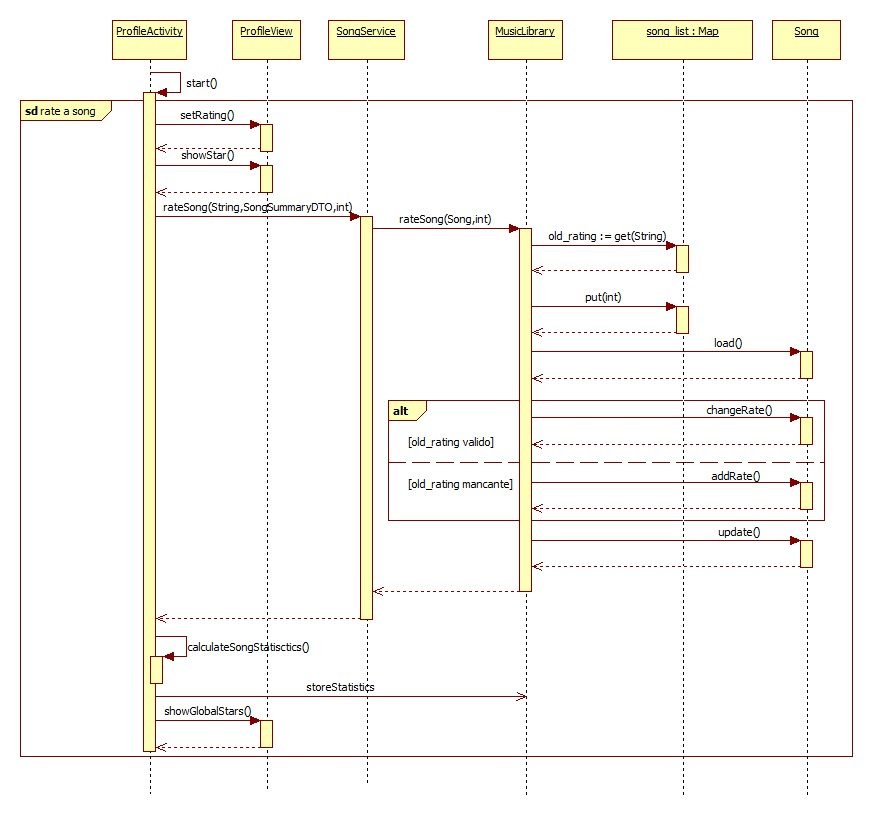
\includegraphics[width=17cm]{img/DP/rate_song.jpg}
\caption{Diagramma UML di sequenza che descrive il procedimento seguito per il
salvataggio di un voto richiesto dall'utente.}
\end{figure}
Il metodo \co{rateSong(String,String,String,int)} contiene una delle funzioni di
\co{ProfileActivity} che necessitano di intevrenire sia in scrittura che in
lettura sul Datastore. Infatti, oltre a salvare il voto assegnato dall'utente,
deve ricevere la nuova media dei voti della canzone alcolata dal server. La
sequenza seguita per svolgere queste operazioni prevede come prima cosa
l'impostazione degli elementi grafici derivanti dalla richiesta dell'utente come
la visualizzazione delle stelline cliccabili \co{showStar()}. Successivamente
avviene la chiamata RPC a \co{SongService} per la scrittua in memoria del voto
assegnato ed il calcolo della nuova media dei voti. Infine l'activity deve
preoccuparsi anche di aggiornare le statistiche, sia su \co{current\_user} sia
nel Datastore tramite \co{storeStatistics}, e aggiornare la grafica con i dati
ricevuti al termine della chiamata RPC.
\begin{longtable}{|p{0.4\textwidth}|p{0.4\textwidth}|}
\hline
\rowcolor{orange} \bo{Attributo} & \bo{Descrizione} \\
\hline
\endhead
\hline
\multicolumn{2}{|c|}{\textit{continua alla pagina successiva}}\\
\hline
\endfoot
\endlastfoot
- client\_factory: ClientFactory & Questo campo serve per aver accesso
al \co{PlaceController}, all'\co{EventBus} e alle varie View.\\\hline
- name: String & Rappresenta il nome
con il quale il \co{ProfilePlace} viene creato.\\\hline
- login\_service\_svc: LoginServiceAsync & Rappresenta la classe Service che ci
permette l'invocazione di metodi remoti (RPC) riguardanti l'attivit\`a
di login.\\\hline
- library\_service\_svc: LibraryServiceAsync & Rappresenta la classe Service che ci
permette l'invocazione di metodi remoti (RPC) riguardanti la libreria
utente.\\\hline
- user\_service\_svc: UserServiceAsync & Rappresenta la classe Service che ci
permette l'invocazione di metodi remoti (RPC) riguardanti l'account
dell'utente.\\\hline
- song\_service\_svc: SongServiceAsync & Rappresenta la classe Service che ci
permette l'invocazione di metodi remoti (RPC) riguardanti i singoli
brani.\\\hline
- current\_user: UserCompleteDTO & Rappresenta il DTO contenente
tutte le informazioni utili al client riguardanti l'account utente e la
sua libreria.\\\hline 
- is\_owner: boolean & Segnala se l'utente \`e o meno il proprietario del
profilo. \\\hline
- info\_alredy\_loaded: Map\textless String, SongDTO\textgreater & Questa mappa,
inizialmente vuota, contiene le informazioni dettagliate di tutte le
canzoni di cui sono gi\`a state richieste attraverso la selezione nella
lista da parte dell'utente.\\\hline
- cover\_alredy\_loaded: Map\textless String, String\textgreater & Questa mappa,
inizialmente vuota, contiene gli indirizzi alle copertine di tutti gli album che
vengono richiesti dall'utente.\\\hline
\# my\_constants: MyConstants &
Questo oggetto ci permetter\`a di internazionalizzare il programma chiamando metodi appositi al posto dell'inserimento di parole String.\\\hline
\caption{Campi dati di ProfileActivity}
\end{longtable}


\begin{longtable}{|p{0.4\textwidth}|p{0.4\textwidth}|}
\hline
\rowcolor{orange} \bo{Metodo} & \bo{Descrizione} \\
\hline
\endhead
\hline
\multicolumn{2}{|c|}{\textit{continua alla pagina successiva}}\\
\hline
\endfoot
\endlastfoot
+ start(AcceptsOneWidget, EventBus) & Invocato da \co{ActivityManager}
per avviare effettivamente una nuova \co{ProfileActivity}\\\hline 
+ goTo(in Place) & Permette di
spostarsi in un place differente anche relativo ad un'altra view. Ad esempio per
tornare alla pagina di \co{LoginView} se l'utente non \`e autenticato. Verr\`a
quindi chiamato nel metodo \emph{start} se un utente tenta di accedere al
ProfileView senza essere autenticato.\\\hline
+ logout() & Effettua il logout dell'utente, facendo scadere la
sessione ed eliminando i cookies relativi ad essa, comunicando con il
\co{LoginService} implementato nel server.\\\hline
+ setPlaylistList() & Deve andare ad invocare il metodo \emph{paintPlaylist} di
\co{ProfileView} per andare a disegnare la lista delle playlist
generata da \emph{getPlaylistList}.\\\hline
+ getPlaylistList() : String[ ] & Crea e restituisce un'array
contenente la lista di playlist dell'utente loggato.\\\hline
+ setFriendList() & Restituisce, dopo aver richiesto le informazioni al
server, la lista degli utenti che hanno una libreria simile a quella
dell'utente.\\\hline 
+ setSongInfo() & Deve andare ad invocare il metodo \emph{setInfo} di
\co{ProfileView} per andare a disegnare le informazioni del brano in
riproduzione accanto al player, fornite da \emph{getSongInfo}.\\\hline
+ getSongInfo() : String & Crea e restituisce le informazioni testuali relative
al brano in riproduzione.\\\hline
+ setPlaylistSongs(in String) & Metodo che riferisce \emph{getPlaylistSongs} per
far disegnare alla \co{ProfileView} la lista dei brani per una certa playlist.\\\hline
+ getPlaylistSongs(in String) & Fa
disegnare alla \co{ProfileView} la lista brani di una playlist tramite
il metodo \emph{paintPlaylistSongs}. I brani vengono recuperati
direttamente nel client senza invocare alcuna RPC.\\\hline 
+ playYouTube(in
String, in String, in String) & Preleva il codice YouTube relativo ad un brano,
dal client se possibile altrimenti dal server, ed invoca \emph{playYouTube}
della View per aprire il player e riprodurlo. Si occupa inoltre di
recuperare la copertina dell'album a cui appartiene la canzone. \\\hline 
+ setSongs() & Utilizzando \emph{getSongs} va a disegnare il catalogo
dell'utente nella View, invocando \emph{paintCatalogo}, inserendo anche la sua dimensione nell'apposito campo.\\\hline + getSongs(in MusicLibraryDTO) : List\textless String\textgreater & Genera e
restituisce la lista di brani del catalogo relativo all'utente loggato.\\\hline
+ addToPLaylist(in String, in String, in String, in String) & Aggiunge
un brano ad una playlist dell'utente, prima localmente sulla view e su
\co{current\_user}, poi aggiornando il dato nel DataStore tramite
\co{library\_service\_svc}.\\\hline  
+ removeFromPLaylist(in String, in String, in String, in String) &
Rimuove un brano da una playlist, prima localmente, poi aggiornando il
DataStore tramite \co{library\_service\_svc}.\\\hline
+ moveUpInPLaylist(in String, in String, in String, in String) & Muove
un brano di una posizione verso l'alto nella playlist, e aggiorna anche
nel DataStore.\\\hline
+ moveDownInPLaylist(in String, in String, in String, in String) & Muove
un brano di una posizione verso il basso nella playlist, e aggiorna anche
nel DataStore.\\\hline
+ addPlaylist(in String) & Aggiunge una nuova playlist nella libreria
dell'utente, se non ne esiste una di ugual nome.\\\hline
+ deletePlaylist(in String) & Elimina irreversibilmente una playlist dalla
libreria utente.\\\hline
+ rateSong(in String, in String, in String, in int) & Assegna un voto
da parte dell'utente ad una canzone aggiornando sia su client che su
server tutti i campi interessati.\\\hline 
+ setRating(in String, in String, in
String) : double & Restituisce il voto complessivo relativo ad una canzone, ed aggiorna inoltre la grafica
con il voto che l'utente ha assegnato per tale brano.\\\hline
+ setSongFields(in String, in String, in String) & Recupera e permette
alla View di disegnare la lista dettagliata di informazioni relative ad una
canzone.\\\hline
+ viewOtherLibrary(in String) & Metodo che permetter\`a di andare a
visualizzare il catalogo di un altro utente NetMus.\\\hline
+ deleteSong(in String, in String, in String) & Elimina una canzone dal
catalogo dell'utente loggato.\\\hline
+ exportDocLibrary() & Richiede al server l'esportazione in Google Doc
del catalogo dell'utente e, una volta generato, lo mostra in una nuova
finestra del browser.\\\hline 
+ editProfileView(in String) & Passa alla View le
informazioni personali relative all'utente loggato.\\\hline + editProfile(in String, in String, in String, in String, in String, in String, in String, in String) & Permette la modifica delle informazioni
dell'utente loggato, inviando i nuovi dati alla View e modificandoli
anche nel DataStore.\\\hline
+ editSongTitle(in String, in String, in String, in String) & Permette
la modifica di un eventuale titolo assente nelle informazioni di un
brano.\\\hline 
+ editSongAlbum(in String, in String, in String, in String) &
Permette la modifica di un eventuale album assente nelle informazioni di un
brano.\\\hline
+ editSongArtist(in String, in String, in String, in String) & Permette
la modifica di un eventuale album assente nelle informazioni di un
brano.\\\hline
+ setSongCover(in String, in String, in String, in HTMLPanel): void & Reperisce
ed assegna al riquadro richiesto nella ``cover mode" della view la copertina
dell'album. \\\hline
+ deleteProfile() & Cancella l'utente definitivamente dal sistema e lo
fa uscire dalla pagina.\\\hline 
+ setStats() & Comunica alla view, tramite il metodo della view \co{setStats}, i
dati rigurdanti la pagina delle statistiche.\\\hline 
+ changeLanguage(in String) & Modifica l'URL del browser per cambiare lingua,
utilizzando la gestione automatica dell'intenazionalizzazione offerta da
GWT.\\\hline
+ mayStop(): String & Fa comparire un pop-up con
un adeguato messaggio ogni qualvolta il browser richiede di uscire dalla pagina. Questo
metodo \`e offerto dalla superclasse \co{Activity}. \\\hline
- calculatePreferredArtist(in Map\textless String, SongSummaryDTO\textgreater): String & Ricerca
all'interno della libreria data in input l'artista pi\`u ricorrente tra tutte le
canzoni.\\\hline
- calculateSongStatistics(in Map\textless String, SongSummaryDTO\textgreater): List\textless
String\textgreater & Ricerca all'interno della libreria data in input la canzone
che \`e stata valutata meglio da tutti gli utenti che la condividono e quella
preferita dall'utente che possiede la libreria. Ne ritorna gli id in una lista.\\\hline
- clearPlaylistName(in String): String & Pulisce i nomi delle playlist
in entrata dalla view poich\'e questi contengono anche il numero di
brani al loro interno.\\\hline
\caption{Metodi di ProfileActivity}
\end{longtable}


\newpage
\section{Package client.place} % LASCIARE WARNING
\subsection*{Requisiti obbligatori soddisfatti}
\begin{itemize}
	\item C1QN-1.6.2 Scalabilit\`a massa di utenza
	\item C1QN-2 Utilizzo
	\item C1VN-2.5 Semplicit\`a di utilizzo
	\item C1QN-2.6 Manutenibilit\`a
\end{itemize}
\subsubsection*{Requisiti desiderabili e opzionali soddisfatti}
\begin{itemize}
    \item Nessuno
\end{itemize}
\subsection*{Tipo, obiettivo e funzione del componente}
Il package contiene le classi di tipo Place. I Place sono indispensabili
per far s\`i che la corrispondente Activity sia accessibile via URL e per
memorizzare i dati relativi allo stato corrente del sistema in modo che siano
rapidamente recuperabili.
\subsection*{Attivit\`a svolte e dati trattati} Organizza i Places.
\subsection{Classe LoginPlace}
\subsubsection*{Requisiti obbligatori soddisfatti}
\begin{itemize}
	\item C1QN-1.6.2 Scalabilit\`a massa di utenza
	\item C1QN-2 Utilizzo
	\item C1VN-2.5 Semplicit\`a di utilizzo
\end{itemize}
\subsubsection*{Requisiti desiderabili e opzionali soddisfatti}
\begin{itemize}
    \item Nessuno
\end{itemize}
\subsubsection*{Tipo, obiettivo e funzione del componente}
\co{LoginPlace} estende la classe \co{Place} messa a disposizione da GWT. La
classe \`e associata alla classe interna \co{Tokenizer} che permette di
serializzare lo stato del Place in un simbolo (token) URL.
Ha la funzione di contenere i dati dello stato corrente della pagina di login.
\subsubsection*{Attivit\`a svolte e dati trattati} Il compito della classe \`e
quello di indicizzare gli stati della pagina di login e mantenerne i dati
finch\'e l'applicazione \`e attiva. Questo permette inoltre di rendere
accessibili le funzionalit\`a di history e bookmarking del browser.
\begin{longtable}{|p{0.4\textwidth}|p{0.4\textwidth}|}
\hline
\rowcolor{orange} \bo{Attributo} & \bo{Descrizione} \\
\hline
\endhead
\hline
\multicolumn{2}{|c|}{\textit{continua alla pagina successiva}}\\
\hline
\endfoot
\endlastfoot
- user: String & Username inserito dall'utente nello stato corrente, sar\`a
diverso da \emph{null} solo nel caso vi si acceda in seguito ad un errore o
dalla history.\\\hline 
- password: String & Password inserita dall'utente nello stato corrente, sar\`a
diversa da \emph{null} solo nel caso vi si acceda in seguito ad un errore o
dalla history.\\\hline 
- error: String & Errore pi\`u rilevante occorso nello stato
corrente, sar\`a diverso da \emph{null} solo nel caso sia avvenuto un
errore nel tentativo di login/registrazione precedente.\\\hline
- login\_type: LoginType & Tipologia di login o registrazione che si sta
effettuando nello stato corrente, di default \`e NETMUSLOGIN.\\\hline
\caption{Campi dati di LoginPlace}
\end{longtable}
\begin{longtable}{|p{0.4\textwidth}|p{0.4\textwidth}|}
\hline
\rowcolor{orange} \bo{Metodo} & \bo{Descrizione} \\
\hline
\endhead
\hline
\multicolumn{2}{|c|}{\textit{continua alla pagina successiva}}\\
\hline
\endfoot
\endlastfoot
+ getUser() : String & Getter dell'attributo \co{user}\\\hline
+ getPassword() : String & Getter dell'attributo \co{password}\\\hline
+ getError() : String & Getter dell'attributo \co{error}\\\hline
+ getLoginType() : LoginType & Getter dell'attributo \co{loginType}\\\hline
\caption{Metodi di LoginPlace}
\end{longtable}

\subsection{Classe ProfilePlace}
\subsubsection*{Requisiti obbligatori soddisfatti}
\begin{itemize}
    \item C1QN-1.6.2 Scalabilit\`a massa di utenza
    \item C1QN-2 Utilizzo
    \item C1VN-2.5 Semplicit\`a di utilizzo
\end{itemize}
\subsubsection*{Requisiti desiderabili e opzionali soddisfatti}
\begin{itemize}
    \item Nessuno
\end{itemize}
\subsubsection*{Tipo, obiettivo e funzione del componente}
\co{ProfilePlace} estende la classe \co{Place} messa a disposizione da GWT. La
classe \`e associata alla classe interna \co{Tokenizer} che permette di
serializzare lo stato del Place in un simbolo (token) URL.
Questa classe contiene un solo attributo di tipo \emph{String} che serve
solamente per generare l'URL della pagina e quindi garantire il funzionamento
della history e dei bookmark dei browser. 
\subsubsection*{Attivit\`a svolte e dati trattati}
Il compito della classe \`e quello di indicizzare gli stati di
\co{ProfileActivity} in modo da rendere accessibili le funzionalit\`a di history
e bookmarking del browser.

\newpage
\begin{longtable}{|p{0.4\textwidth}|p{0.4\textwidth}|}
\hline
\rowcolor{orange} \bo{Attributo} & \bo{Descrizione} \\
\hline
\endhead
\hline
\multicolumn{2}{|c|}{\textit{continua alla pagina successiva}}\\
\hline
\endfoot
\endlastfoot
- profile\_name: String & Username dell'utente a cui appartiene il
profilo. Questo nome viene utilizzato per determinare l'URL che
rappresenta lo stato attuale della pagina.\\\hline
\caption{Campi dati di ProfilePlace}
\end{longtable}

\begin{longtable}{|p{0.4\textwidth}|p{0.4\textwidth}|}
\hline
\rowcolor{orange} \bo{Metodo} & \bo{Descrizione} \\
\hline
\endhead
\hline
\multicolumn{2}{|c|}{\textit{continua alla pagina successiva}}\\
\hline
\endfoot
\endlastfoot
+ getProfileName() : String & Getter dell'attributo \co{profile\_name}.\\\hline
\caption{Metodi di ProfilePlace}
\end{longtable}


\newpage
\section{Package client.mvp}
\subsection*{Requisiti obbligatori soddisfatti}
\begin{itemize}
    \item C1QN-2.6 Manutenibilit\`a
\end{itemize}
\subsection*{Requisiti desiderabili e opzionali soddisfatti}
\begin{itemize}
    \item Nessuno
\end{itemize}
\subsection*{Tipo, obiettivo e funzione del componente}
Questo package racchiude le classi di gestione di Activity e Place implementate
dal framework di GWT2.1 ``MVP with Activities and Places''. Questo package \`e
fondamentale per le funzionalit\`a di gestione della history e del bookmarking
da parte dei browser.
\subsection*{Attivit\`a svolte e dati trattati}
Gestisce il collegamento tra Place e Activity per abilitare le funzioni di
history, bookmarking e mantenimento dello stato del client.

\subsection{Classe NetmusActivityMapper}
\subsubsection*{Requisiti obbligatori soddisfatti}
\begin{itemize}
	\item C1QN-2 Utilizzo
	\item C1QN-2.6 Manutenibilit\`a
\end{itemize}
\subsubsection*{Requisiti desiderabili e opzionali soddisfatti}
\begin{itemize}
    \item Nessuno
\end{itemize}
\subsubsection*{Tipo, obiettivo e funzione del componente}
Questa classe si occupa di mappare ogni attivit\`a con il corrispondente Place.
\subsubsection*{Attivit\`a svolte e dati trattati}
Tramite un riferimento ad un Place crea e restituisce un oggetto activity.
\begin{longtable}{|p{0.4\textwidth}|p{0.4\textwidth}|}
\hline
\rowcolor{orange} \bo{Attributo} & \bo{Descrizione} \\
\hline
\endhead
\hline
\multicolumn{2}{|c|}{\textit{continua alla pagina successiva}}\\
\hline
\endfoot
\endlastfoot
- client\_factory: ClientFactory & Factory che deve essere passata a tutte
le attivit\`a instanziate in questa classe. \\\hline
\caption{Campi dati di NetmusActivityMapper}
\end{longtable}
\begin{longtable}{|p{0.4\textwidth}|p{0.4\textwidth}|}
\hline
\rowcolor{orange} \bo{Metodo} & \bo{Descrizione} \\
\hline
\endhead
\hline
\multicolumn{2}{|c|}{\textit{continua alla pagina successiva}}\\
\hline
\endfoot
\endlastfoot
+ getActivity(in Place): Activity & Mappa e istanzia l'activity adeguata
in base al tipo del place dato in input.\\
& \co{LoginPlace}-\co{LoginActivity}\\ 
& \co{ProfilePlace}-\co{ProfileActivity}\\
& \co{EditSongsPlace}-\co{EditSongsActivity}\\
& \co{EditProfilePlace}-\co{EditProfileActivity}\\\hline
\caption{Metodi di NetmusActivityMapper}
\end{longtable}


\subsection{Classe NetmusPlaceHistoryMapper}
\subsubsection*{Requisiti obbligatori soddisfatti}
\begin{itemize}
    \item C1QN-2 Utilizzo
    \item C1QN-2.6 Manutenibilit\`a
\end{itemize}
\subsubsection*{Requisiti desiderabili e opzionali soddisfatti}
\begin{itemize}
    \item Nessuno
\end{itemize}
\subsubsection*{Tipo, obiettivo e funzione del componente}
Dichiara e riferisce tutti i places che saranno utilizzati da NetMus.
\subsubsection*{Attivit\`a svolte e dati trattati}
Funge da connessione tra i PlaceTokenizer (classe interna ad ogni Place) e il
PlaceHistoryHandler (messo a disposizione da GWT) che sincronizza l'URL del
browser con i vari Place.
\begin{longtable}{|p{0.4\textwidth}|p{0.4\textwidth}|}
\hline
\rowcolor{orange} \bo{Metodo} & \bo{Descrizione} \\
\hline
\endhead
\hline
\multicolumn{2}{|c|}{\textit{continua alla pagina successiva}}\\
\hline
\endfoot
\endlastfoot
@WithTokenizers \begin{verbatim}(LoginPlace.Tokenizer.class,
ProfilePlace.Tokenizer.class,
EditUserPlace.Tokenizer.class,
EditSongsPlace.Tokenizer.class)\end{verbatim} & Questa annotazione che precede
la definizione dell'interfaccia permette di associare ogni place al \co{PlaceHistoryHandler} e quindi risparmia
la dichiarazione esplicita di attributi e metodi per l'implementazione
di un \co{TokenizerFactory} separato.\\\hline
\caption{Metodi di NetmusPlaceHistoryMapper}
\end{longtable}


\newpage
\section{Package client.service} % LASCIARE WARNING
\subsection*{Requisiti obbligatori soddisfatti}
\begin{itemize}
    \item C1FN-1 Web Application NetMus
    \item C1VN-1.11 Deve utilizzare il cloud computing
    \item C1VN-1.12 Deve utilizzare tecnologie GAE e GWT
    \item C1QN-2.6 Manutenibilit\`a
\end{itemize}
\subsubsection*{Requisiti desiderabili e opzionali soddisfatti}
\begin{itemize}
    \item Nessuno
\end{itemize}
\subsection*{Tipo, obiettivo e funzione del componente}
Il contenuto di questo package \`e di fondamentale importanza poich\'e
rappresenta la parte client del framework RPC che viene utilizzato per scambio
di oggetti tra client e server. \co{client.service} \`e costituito da tutte
le interfacce dei servizi remoti offerti dal server. Le funzionalit\`a delle
classi in esso contenute saranno divise in base al tipo di servizio offerto. Per
ognuno di questi sar\`a presente un'interfaccia normale (che estende
\co{RemoteService}) e un'interfaccia \bo{asincrona}.
\subsection*{Attivit\`a svolte e dati trattati}
Vengono forniti tutti i servizi che il server sar\`a in grado di dare, i dati
trattati saranno i DTO definiti nel package \emph{shared}.\\\\
\underline{I metodi sono presentati nelle rispettive classi implementazione
descritte nel paragrafo 4.9.}

\subsection{Interfaccia SongService (e SongServiceAsync)}
\subsubsection*{Requisiti obbligatori soddisfatti}
\begin{itemize}
	\item C1QN-1.6 Scalabilit\`a
\end{itemize}
\subsubsection*{Requisiti desiderabili e opzionali soddisfatti}
\begin{itemize}
    \item C1FD-1.1.4 Visualizza player YouTube
    \item C1FD-1.3 Personalizzazione del catalogo
    \item C1FD-1.3.1 Cancellazione brano
    \item C1FO-1.3.4 Ranking brani
    \item C1FD-1.5 Riproduzione tracce in streaming
    \item C1QD-1.5.1 Ottimizzazione della ricerca su YouTube
\end{itemize}
\subsubsection*{Tipo, obiettivo e funzione del componente}
Questa classe dovr\`a consentire alle componenti Activity di \emph{client} di
inviare richieste di vario tipo a \emph{server} riguardanti informazioni sui
brani musicali. Le richieste in questione dovranno tenere in considerazione il
fatto che ogni brano pu\`o essere condiviso da molti utenti e la modifica di
quest'ultimo \`e molto delicata da gestire, per questo motivo si far\`a ricorso a
questi servizi solo se strettamente necessario. Sar\`a presente anche
\co{SongServiceAsync}, che gestir\`a il ritorno dai metodi in maniera asincrona.
\subsubsection*{Attivit\`a svolte e dati trattati}
Questa interfaccia fornir\`a l'accesso a servizi per interagire con i brani
salvati nel DataStore e condivisi da pi\`u utenti. Utilizzer\`a dati di tipo
SongDTO e SongSummaryDTO.\\\\ \underline{I metodi sono presentati nella
rispettiva classe implementazione descritta nel paragrafo 4.9.1.}

\subsection{Interfaccia UserService (e UsersServiceAsync)}
\subsubsection*{Requisiti obbligatori soddisfatti}
\begin{itemize}
	\item C1FN-1.4 Gestione profilo personale
	\item C1FN-1.4.1 Modifica informazioni personali
	\item C1FN-1.4.2 Cambio password
	\item C1FN-1.4.3 Cancellazione del proprio account
    \item C1QN-1.6 Scalabilit\`a
\end{itemize}
\subsubsection*{Requisiti desiderabili e opzionali soddisfatti}
\begin{itemize}
    \item C1FD-1.3 Personalizzazione del catalogo
    \item C1FD-1.7 Interazione con altri utenti
    \item C1FD-1.7.1 Visualizzazione altri profili
\end{itemize}
\subsubsection*{Tipo, obiettivo e funzione del componente}
Questa classe consentir\`a alle componenti Activity di \emph{client} di inviare
richieste di vario tipo a \emph{server} riguardanti le informazioni personali
dell'utente da mostrare nell'interfaccia grafica. Le funzionalit\`a comprese in
questi servizi saranno solamente quelle basilari ovvero l'inserimento, la
modifica e la cancellazione di un utente. Sar\`a presente
anche \co{UsersServiceAsync}, che gestir\`a il ritorno dai metodi in maniera
asincrona. 
\subsubsection*{Attivit\`a svolte e dati trattati}
Questa interfaccia fornir\`a l'accesso a servizi per richiedere o
modificare (quando possibile) qualsiasi tipo di informazione riguardante gli
utenti del sistema e utilizzer\`a dati di tipo \co{UserDTO}
e \co{UserCompleteDTO}.\\\\
\underline{I metodi sono presentati nella rispettiva classe implementazione
descritta nel paragrafo 4.9.2.}

\subsection{Interfaccia LibraryService (e LibraryServiceAsync)}
\subsubsection*{Requisiti obbligatori soddisfatti}
\begin{itemize}
    \item C1QN-1.6 Scalabilit\`a
    \item C1FN-1.9 Ricezione ed elaborazione dei brani
    \item C1FN-1.9.1 Controllo di validit\`a dei dati
\end{itemize}
\subsubsection*{Requisiti desiderabili e opzionali soddisfatti}
\begin{itemize}
    \item C1FD-1.3 Personalizzazione del catalogo
    \item C1FO-1.3.3 Creazione playlist
    \item C1FO-1.3.4 Ranking brani
    \item C1FD-1.8 Elaborazione dati utente
    \item C1FO-1.8.1 Esportazione PDF
    \item C1FO-1.9.3 Completamento info da servizio esterno
\end{itemize}
\subsubsection*{Tipo, obiettivo e funzione del componente}
Questa classe consentir\`a alle componenti Activity di \emph{client} di inviare
richieste di vario tipo a \emph{server} riguardanti il catalogo musicale utente
da mostrare nell'interfaccia grafica. Qui vengono definiti molti dei servizi
principali offerti da NetMus, in particolare l'inserimento di nuove canzoni nel
DataStore con la chiamata asincrona \emph{sendUserNewMusic}. Le
funzionalit\`a di gestione delle playlist e delle statistiche del
catalogo sono interamente racchiuse in questa classe. Sar\`a presente anche
\co{LibraryServiceAsync}, che gestir\`a il ritorno dai metodi in maniera asincrona. 
\subsubsection*{Attivit\`a svolte e dati trattati}
Questa interfaccia fornir\`a l'accesso a servizi per richiedere qualsiasi tipo
di informazione riguardante la libreria musicale utente e utilizzer\`a dati di
tipo \co{MusicLibraryDTO}.\\\\
\underline{I metodi sono presentati nella rispettiva classe implementazione
descritta nel paragrafo 4.9.3.}


\subsection{Interfaccia LoginService (e LoginServiceAsync)}
\subsubsection*{Requisiti obbligatori soddisfatti}
\begin{itemize}
	\item C1FN-1.2 Registrazione
	\item C1QN-1.6 Scalabilit\`a
\end{itemize}
\subsubsection*{Requisiti desiderabili e opzionali soddisfatti}
\begin{itemize}
    \item C1FO-1.2.1 Pagina login indipendente
\end{itemize}
\subsubsection*{Tipo, obiettivo e funzione del componente}
\co{LoginService} mette a disposizione metodi
che soddisfano le possibili richieste verso la parte model riguardanti l'autenticazione degli utenti.
Questi metodi si occupano inoltre di gestire la parte relativa alle sessioni HTTP. 
\`E presente anche \co{LoginServiceAsync}, che gestisce il ritorno dai
metodi in maniera asincrona.
\subsubsection*{Attivit\`a svolte e dati trattati}
Questa interfaccia fornisce l'accesso a servizi per richiedere qualsiasi tipo
di informazione riguardante l'autenticazione dell'utente al sistema
e utilizza dati di tipo \co{LoginDTO}.
Gli attributi e i metodi di questa interfaccia verranno descritti nel
dettaglio nella classe \co{LoginServiceImpl} che li implementa. \\\\
\underline{I metodi sono presentati nella rispettiva classe implementazione
descritta nel paragrafo 4.9.4.}


\newpage
\section{Package client.applet} % LASCIARE WARNING

\begin{figure}[h]
  \centering
  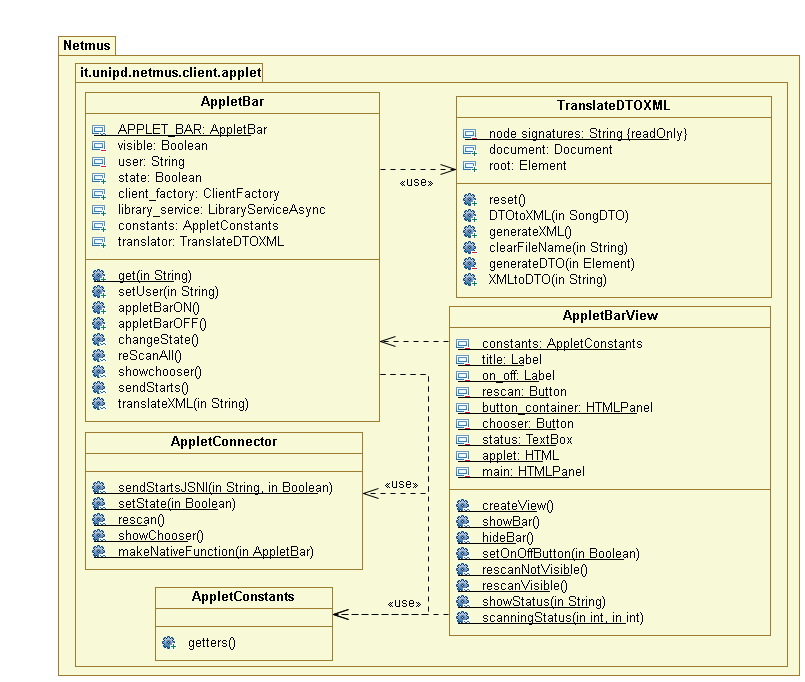
\includegraphics[width=13cm]{img/DP/netmus_client_applet.png}
\caption{Diagramma UML delle classi che descrive le dipendenze
fondamentali presenti all'interno del package
\emph{it.unipd.netmus.client.applet.}}
\end{figure}


\subsection*{Requisiti obbligatori soddisfatti}
\begin{itemize}
    \item C1FN-1.9 Ricezione ed elaborazione dei brani
    \item C2FN-3 Comunicazione con C1
    \item C2QN-4.4 Utilizzo
    \item C2VN-4.6 Norme legali
\end{itemize}
\subsection*{Requisiti desiderabili e opzionali soddisfatti}
\begin{itemize}
    \item Nessuno
\end{itemize}
\subsection*{Obiettivo e funzione del componente}
Questo package conterr\`a le classi necessarie a gestire richieste e segnali
provenienti dalla applet precompilata, che andremo ad inserire nel programma.
Tale applet avr\`a la funzione di effettuare la scansione e l'estrazione
automatica dei tag dei file musicali mp3, presenti nei dispositivi di
archiviazione di massa che vengono collegati alla macchina dell'utente.\\
Per comunicare con tale applet sono state valutate due possibili metodologie
d'implementazione: l'uso di una libreria che crea un sistema proxy tra la applet
e GWT oppure l'utilizzo di \underline{JSNI} (JavaScript Native Interface) che
sostanzialmente ci permette di effettuare chiamate di metodi da JavaScript al
codice \underline{Java} e viceversa: abbiamo utilizzato quest'ultima opzione.
\subsection*{Meccanismo di lavoro del componente}
Una volta ricevuta una richiesta da parte della applet, verr\`a creata
una lista di \co{SongDTO} dalla stringa XML ricevuta che verr\`a poi inviata al
server tramite \co{LibraryService} il quale elaborer\`a i dati, memorizzandoli
nel DataStore ed associandoli all'utente.\\
In particolare, lo scambio delle informazioni dei brani tra applet e questo
package avviene utilizzando \underline{XML}, permettendo quindi di contenere
tutte le informazioni necessarie all'interno di un'unica stringa, in maniera da
aggirare molte difficolt\`a e limiti derivanti dall'utilizzo di JSNI.

\subsection{Classe TranslateDTOXML}
\subsubsection*{Requisiti obbligatori soddisfatti}
\begin{itemize}
    \item C1FN-1.9 Ricezione ed elaborazione dei brani
    \item C1FN-1.9.5 Inserimento nel Database
    \item C2FN-3 Comunicazione con C1
\end{itemize}
\subsubsection*{Requisiti desiderabili e opzionali soddisfatti}
\begin{itemize}
    \item Nessuno
\end{itemize}
\subsubsection*{Tipo, obiettivo e funzione del componente}
Si occupa di interpretare le informazioni in formato XML ricevute dall'applet,
generando i relativi DTO contenenti le informazioni. Pu\`o effettuare anche
l'operazione inversa, ovvero generare una stringa in formato XML che rappresenta
le informazioni contenute nei DTO.
\subsubsection*{Attivit\`a svolte e dati trattati}
Interpretazione e traduzione delle informazioni dei brani da XML a DTO e
viceversa.
\begin{longtable}{|p{0.4\textwidth}|p{0.4\textwidth}|}
\hline
\rowcolor{orange} \bo{Attributo} & \bo{Descrizione} \\
\hline
\endhead
\hline
\multicolumn{2}{|c|}{\textit{continua alla pagina successiva}}\\
\hline
\endfoot
\endlastfoot
- ROOT\_NAME: String \emph{static final} & Nome del nodo principale nel
documento XML.\\\hline
- SONG\_NAME: String \emph{static final} & Nome del nodo nel documento XML
riguardante una singola canzone.\\\hline
- ALBUMTITLE\_NAME: String \emph{static final} & Nome del nodo nel documento XML
riguardante il titolo dell'album.\\\hline
- AUTHORCOMPOSER\_NAME: String \emph{static final} & Nome del nodo nel documento
XML riguardante il compositore.\\\hline
- LEADARTIST\_NAME: String \emph{static final} & Nome del nodo nel documento XML
riguardante l'artista.\\\hline
- SONGGENRE\_NAME: String \emph{static final} & Nome del nodo nel documento XML
riguardante il genere musicale del brano.\\\hline
- SONGTITLE\_NAME: String \emph{static final} & Nome del nodo nel documento XML
riguardante il titolo del brano.\\\hline
- TRACKNUMBER\_NAME: String \emph{static final} & Nome del nodo nel documento
XML riguardante il numero della traccia all'interno dell'album.\\\hline
- YEAR\_NAME: String \emph{static final} & Nome del nodo nel documento XML
riguardante l'anno di uscita del brano.\\\hline
- FILE\_NAME: String \emph{static final} & Nome del nodo nel documento XML
riguardante il file MP3.\\\hline
- document: Document & Documento corrente dal quale si stanno ricavando
i SongDTO.\\\hline 
- root: Element & Elemento (nodo) principale del documento,
che contiene tutti gli altri.\\\hline
\caption{Campi dati di TranslateDTOXML}
\end{longtable}
\begin{longtable}{|p{0.4\textwidth}|p{0.4\textwidth}|}
\hline
\rowcolor{orange} \bo{Metodo} & \bo{Descrizione} \\
\hline
\endhead
\hline
\multicolumn{2}{|c|}{\textit{continua alla pagina successiva}}\\
\hline
\endfoot
\endlastfoot
- generateDTO(in Element): SongDTO & Crea un nuovo SongDTO, e seguendo
le propriet\`a indicate nel nodo di tipo Song, imposta opportunamente i suoi
attributi.\\\hline
+ XMLToDTO(in String): List\textless SongDTO\textgreater & Fa il parsing del
documento XML, e per ogni nodo di tipo Song, utilizza \co{generateDTO} per
creare il relativo SongDTO, e se lo salva su una lista.\\\hline
\caption{Metodi di TranslateDTOXML}
\end{longtable}

\subsection{Classe AppletConstants}
\subsubsection*{Requisiti obbligatori soddisfatti}
\begin{itemize}
    \item C2QN-4 Utilizzo
\end{itemize}
\subsubsection*{Requisiti desiderabili e opzionali soddisfatti}
\begin{itemize}
    \item C1QD-2.4 Supporto multi-lingua
    \item C2QD-4.3 Supporto multi-lingua
\end{itemize}
\subsubsection*{Tipo, obiettivo e funzione del componente}
Gestisce la traduzione delle frasi e/o avvisi da mostrare all'utente, a seconda
della lingua correntemente selezionata, utilizzando un meccanismo proprio di
GWT.
\subsubsection*{Attivit\`a svolte e dati trattati}
Utilizza i file \co{.properties} presenti in questo package, ognuno dei quali
definisce la traduzione corretta di ogni termine e/o frase in una determinata
lingua.
Una volta definita globalmente la lingua utilizzata, viene caricato
automaticamente il file contenente le definizioni di quella lingua.
\begin{longtable}{|p{0.4\textwidth}|p{0.4\textwidth}|}
\hline
\rowcolor{orange} \bo{Metodo} & \bo{Descrizione} \\
\hline
\endhead
\hline
\multicolumn{2}{|c|}{\textit{continua alla pagina successiva}}\\
\hline
\endfoot
\endlastfoot
\# testi\_vari(): String & Questa classe contiene tutti i metodi che
vengono invocati al posto dell'inserimento di un normale testo statico nelle
classi di \emph{applet}, per poter restituire una parola nella giusta
lingua (definita dal parametro ?locale= presente nell'URL).\\\hline
\caption{Metodi di AppletConstants}
\end{longtable}

\subsection{Classe AppletBar}
\subsubsection*{Requisiti obbligatori soddisfatti}
\begin{itemize}
    \item C1FN-1.9 Ricezione ed elaborazione dei brani
    \item C1FN-1.9.1 Controllo di validit\`a dei dati
    \item C1QN-2 Utilizzo
    \item C2FN-1.2 Recupero manuale
    \item C2FN-3 Comunicazione con C1
\end{itemize}
\subsubsection*{Requisiti desiderabili e opzionali soddisfatti}
\begin{itemize}
    \item Nessuno
\end{itemize}
\subsubsection*{Tipo, obiettivo e funzione del componente}
Si occupa di interfacciare utente, servizi ed applet tra loro: in particolare,
comunica visivamente all'utente lo stato dell'applet tramite \co{AppletBarView},
e utilizza i servizi del server per salvare le informazioni estratte da quest'ultima.
Definisce i metodi JSNI per la comunicazione con l'applet utilizzando
\co{AppletConnector}. Utilizza il pattern Singleton.
\subsubsection*{Attivit\`a svolte e dati trattati}
Si occupa di gestire l'applet all'interno del programma: questo prevede il
caricamento del suo codice e la sua inizializzazione, la ricezione delle
informazioni dei brani e l'invio degli stessi a \emph{server} una volta
costruiti i relativi DTO, la visualizzazione dello stato all'utente e i
controlli necessari ad influenzarne il comportamento.
\begin{longtable}{|p{0.4\textwidth}|p{0.4\textwidth}|}
\hline
\rowcolor{orange} \bo{Attributo} & \bo{Descrizione} \\
\hline
\endhead
\hline
\multicolumn{2}{|c|}{\textit{continua alla pagina successiva}}\\
\hline
\endfoot
\endlastfoot
\# APPLET\_BAR: AppletBar \emph{static} & Istanza corrente di AppletBar.\\\hline
- visible: boolean & Indica se l'applet \`e caricata o no.\\\hline
- user: String & Identificativo dell'utente.\\\hline
- state: boolean & Indica se la scansione automatica \`e attiva o no.\\\hline
- client\_factory: ClientFactory & Istanza di ClientFactory usata per accedere
all'EventBus.\\\hline
- library\_service: LibraryServiceAsync & Servizio del server utilizzato per
caricare i nuovi brani.\\\hline 
- constants: AppletConstants \emph{static} & Utilizzato per la
traduzione in pi\`u lingue.\\\hline
- translator: TranslateDTOXML & Utilizzato per tradurre un documento XML
in una lista di SongDTO.\\\hline
\caption{Campi dati di AppletBar}
\end{longtable}
\begin{longtable}{|p{0.4\textwidth}|p{0.4\textwidth}|}
\hline
\rowcolor{orange} \bo{Metodo} & \bo{Descrizione} \\
\hline
\endhead
\hline
\multicolumn{2}{|c|}{\textit{continua alla pagina successiva}}\\
\hline
\endfoot
\endlastfoot
+ get(in String): AppletBar \emph{static} & Se non esiste gi\`a, crea una nuova
istanza di AppletBar e la salva nel relativo campo statico. Restituisce
l'istanza dopo aver aggiornato l'utente.\\\hline 
- AppletBar(in String) & Costruttore di AppletBar, inizializza view e
funzioni.\\\hline 
- setUser(in String) & Aggiorna l'attributo user.\\\hline
+ appletBarON() & Crea il men\`u laterale.\\\hline 
+ appletBarOFF() & Elimina il men\`u laterale.\\\hline
\# changeState() & Attiva/disattiva la scansione automatica, e aggiorna
view e applet di conseguenza.\\\hline 
\# reScanAll() & Indica all'applet di riscansionare l'ultimo device.\\\hline
\# showChooser() & Indica all'applet di effettuare una scansione
manuale.\\\hline 
\# sendStarts() & Inizializza l'applet.\\\hline 
\# translateXML(in String) & Dall'XML ricevuto, fa partire la catena di chiamate
a sendMusic( .\\\hline
- sendMusic(in String) & Questo metodo si occupa di mandare al server le SongDTO
grazie a LibraryService, una volta estratte e create dall'XML, il tutto 30
brani alla volta per evitare problemi di timeout delle GWT-RPC.\\\hline
\caption{Metodi di AppletBar}
\end{longtable}

\subsection{Classe AppletBarView}
\subsubsection*{Requisiti obbligatori soddisfatti}
\begin{itemize} 
    \item C1FN-1.1.2 Menu laterali
    \item C1QN-2 Utilizzo
    \item C1QN-2.3 Portabilit\`a
    \item C1VN-2.5 Semplicit\`a di utilizzo
    \item C2FN-1.2 Recupero manuale
    \item C2QN-4 Utilizzo
\end{itemize}
\subsubsection*{Requisiti desiderabili e opzionali soddisfatti}
\begin{itemize}
    \item Nessuno
\end{itemize}
\subsubsection*{Tipo, obiettivo e funzione del componente}
Interfaccia grafica: si occupa dell'interazione con l'utente.
\subsubsection*{Attivit\`a svolte e dati trattati}
Mostra all'utente lo stato dell'applet, e gli fornisce gli elementi per
interagire con essa.
\begin{longtable}{|p{0.4\textwidth}|p{0.4\textwidth}|}
\hline
\rowcolor{orange} \bo{Attributo} & \bo{Descrizione} \\
\hline
\endhead
\hline
\multicolumn{2}{|c|}{\textit{continua alla pagina successiva}}\\
\hline
\endfoot
\endlastfoot
- constants: AppletConstants \emph{static} & Oggetto utilizzato per la
traduzione nella lingua corretta.\\\hline 
- title: Label \emph{static} & Visualizza il nome del men\`u laterale.\\\hline 
- on\_off: Label \emph{static} & Visualizza se la scansione automatica
\`e attivata o no, e di cambiare questa opzione.\\\hline 
- rescan: Button \emph{static} & Permette di far riscansionare l'ultimo
device: \`e visibile solo dopo una scansione.\\\hline 
- button\_container: HTMLPanel \emph{static} & Contenitore per i pulsanti
.\\\hline 
- chooser: Button \emph{static} & Permette all'utente di far
scansionare una cartella specifica.\\\hline
- status: TextBox \emph{static} & Mostra visivamente lo stato
dell'applet.\\\hline
- applet: HTML \emph{static} & Contiene l'applet.\\\hline
- main: HTMLPanel \emph{static} & Contiene tutta questa view.\\\hline

\caption{Campi dati di AppletBarView}
\end{longtable}
\begin{longtable}{|p{0.4\textwidth}|p{0.4\textwidth}|}
\hline
\rowcolor{orange} \bo{Metodo} & \bo{Descrizione} \\
\hline
\endhead
\hline
\multicolumn{2}{|c|}{\textit{continua alla pagina successiva}}\\
\hline
\endfoot
\endlastfoot
\# createView() \emph{static} & Inizializza e crea la view.\\\hline
\# showBar() \emph{static} & Rende visibile la view e carica il codice
dell'applet.\\\hline 
\# hideBar() \emph{static} & Rende non visibile la view e toglie il codice
dell'applet.\\\hline 
\# setOnOffButton(in boolean) \emph{static} & Cambia lo stato del pulsante
on\_off.\\\hline 
\# rescanNotVisible() \emph{static} & Nasconde il pulsante rescan.\\\hline 
\# rescanVisible() \emph{static} & Visualizza il pulsante rescan.\\\hline 
\# showStatus(in String) \emph{static} & Visualizza lo stato
dell'applet.\\\hline 
\# scanningStatus(in int,in int) \emph{static} & Visualizza lo stato
della scansione: scansionati m su n.\\\hline
\caption{Metodi di AppletBarViews}
\end{longtable}

\subsection{Classe AppletBarConnector}

\begin{figure}[h]
  \centering
  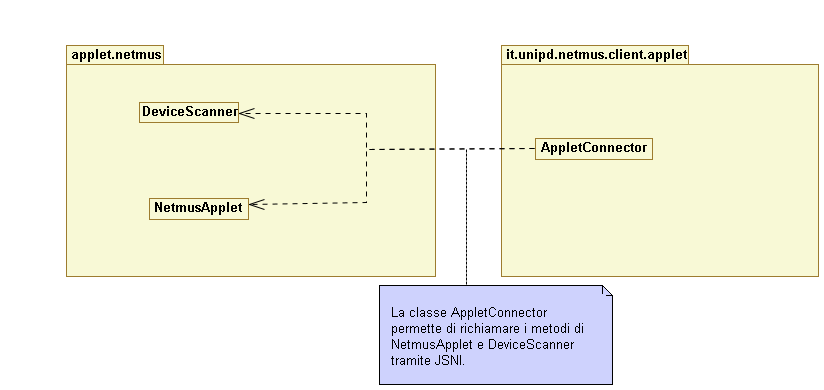
\includegraphics[width=11cm]{img/DP/applet_gwt.png}
\caption{Diagramma UML che descrive le dipendenze e i meccanismi di
connessione tra l'applet e le classi NetMus.}
\end{figure}


\subsubsection*{Requisiti obbligatori soddisfatti}
\begin{itemize} 
    \item C1FN-1.9 Ricezione ed elaborazione dei brani
    \item C1QN-2.6 Manutenibilit\`a
\end{itemize}
\subsubsection*{Requisiti desiderabili e opzionali soddisfatti}
\begin{itemize}
    \item Nessuno
\end{itemize}
\subsubsection*{Tipo, obiettivo e funzione del componente}
Effettua l'interfacciamento tra l'applet e AppletBar, utilizzando JSNI.
\subsubsection*{Attivit\`a svolte e dati trattati}
Dichiara dei metodi globali in JavaScript che hanno il compito di reindirizzare
le chiamate dell'applet all'istanza di \co{AppletBar}.
D'altro canto, implementa anche i metodi nativi per permettere ad \co{AppletBar}
di richiamare metodi sull'applet.
\begin{longtable}{|p{0.4\textwidth}|p{0.4\textwidth}|}
\hline
\rowcolor{orange} \bo{Metodo} & \bo{Descrizione} \\
\hline
\endhead
\hline
\multicolumn{2}{|c|}{\textit{continua alla pagina successiva}}\\
\hline
\endfoot
\endlastfoot
\# sendStartsJSNI(in String, in boolean) \emph{static native} &
Inizializza l'applet.\\\hline 
\# setState(in boolean) \emph{static native} & Attiva/disattiva la scansione
automatica\\\hline 
\# sendRescan() \emph{static native} & Indica all'applet di fare una
scansione completa dell'ultimo device utilizzato.\\\hline 
\# showChooser() \emph{static native} & Indica all'applet di fare una
scansione manuale di una cartella indicata dall'utente. Si occupa
l'applet di chiedere quale.\\\hline 
\# makeNativeFunction(in AppletBar) \emph{static native} & Crea delle
funzioni JavaScript utilizzabili dall'applet, che richiamano i metodi
relativi di AppletBar.\\\hline
\caption{Metodi di AppletConnector}
\end{longtable}

\newpage
\subsection{Dettaglio elaborazione brani ricevuti dall'applet}

\begin{figure}[!h]
  \centering
  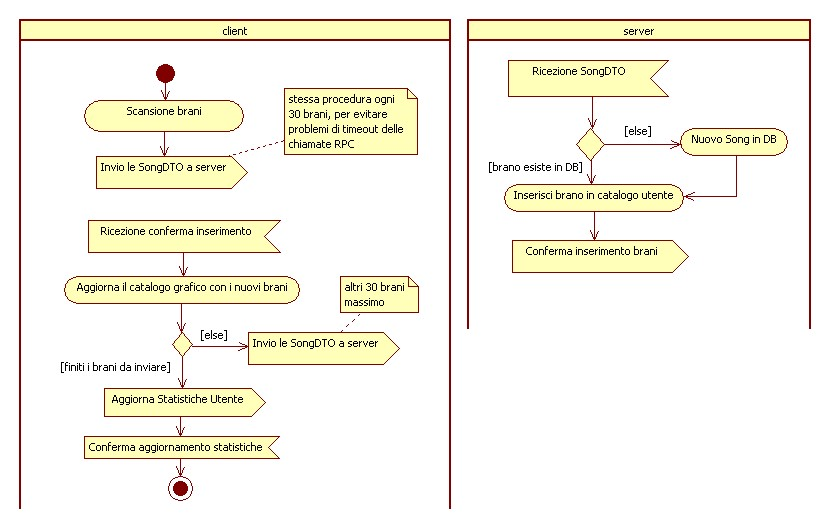
\includegraphics[width=17cm]{img/DP/activity_elab_brani.png}
\caption{Diagramma delle attivit\`a che descrive l'elaborazione dei brani una
volta estratti dall'applet.}
\end{figure}

In questo diagramma viene spiegato il procedimento logico per andare ad
elaborare i brani una volta estratti dall'applet di estrazione e passati ad
\co{AppletBar}.\\\\
Quando arriva la stringa dall'applet contenente il codice XML di tutti i brani
estratti, vengono elaborati 30 brani alla volta creando liste di SongDTO.
Queste vengono inviate al server, che si occuper\`a di controllare per ogni
SongDTO se esiste un Song che gi\`a lo rappresenta nel DataStore. Se non esiste
lo crea. Una volta confermata l'esistenza di tale Song nel DataStore viene
inserito (associato) tale brano nella libreria dell'utente e quindi ritorna al
client conferma di tale operazione.\\\\
Dopodich\`e il client aggiorna la libreria grafica con i nuovi brani inseriti e
continua a ripetere questo procedimento fino ad aver `svuotato` il file
XML.\\
Al termine di tale procedura, vengono aggiornati i dati statistici
dell'utente, e vengono sincronizzati nel client.

\newpage
\begin{figure}[!h]
  \centering
  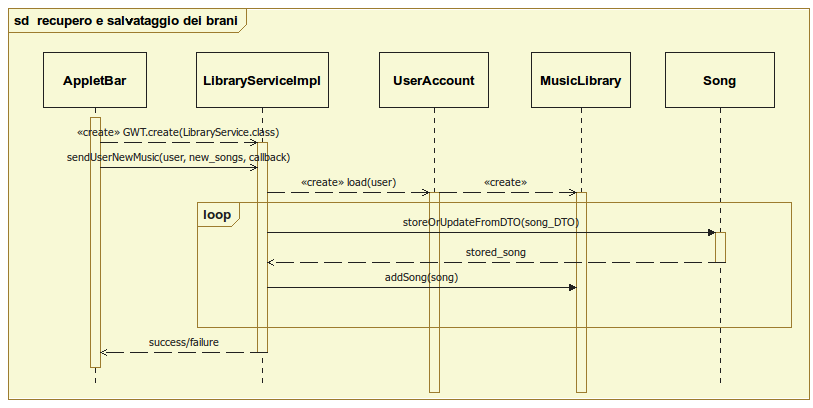
\includegraphics[width=17cm]{img/DP/sequences.png}
\caption{Diagramma UML di sequenza che spiega come vengono memorizzati i brani
in entrata da applet.}
\end{figure}

Questo diagramma mostra nello specifico come vengono memorizzati nel DataStore i
brani in arrivo da applet.\\
Si pu\`o vedere come prima di tutto venga elaborata la singola canzone in base
al contenuto del DataStore e poi venga associata alla libreria dell'utente.\\\\
Il sendUserNewMusic viene chiamato ogni massimo 30 SongDTO da elaborare.
Altrimenti potrebbero esserci problemi di Timeout delle GWT-RPC.


\newpage
\section{Package client.event}
\subsection*{Requisiti obbligatori soddisfatti}
\begin{itemize}
    \item C1FN-1.1 Web Application NetMus
    \item C1FN-1.1.1 Brani elencati opportunamente
    \item C1FN-1.9 Ricezione ed elaborazione dei brani
\end{itemize}
\subsection*{Requisiti desiderabili e opzionali soddisfatti}
\begin{itemize}
    \item Nessuno
\end{itemize}
\subsection*{Tipo, obiettivo e funzione del componente}
Questo package conterr\`a le classi che rappresenteranno i nostri eventi
personalizzati, utilizzabili potenzialmente in tutto il \co{client}.
Questi eventi potranno essere lanciati sull'EventBus ed essere catturati e
gestiti in ogni classe avente accesso all'EventBus tramite \co{ClientFactory}.
\subsection*{Attivit\`a svolte e dati trattati}
Glie eventi svolgono la funzione di segnale, per dare l'input d'inizio ad un
qualche procedimento.

\subsection{Classe DeviceScannedEvent}
\subsubsection*{Requisiti obbligatori soddisfatti}
\begin{itemize}
    \item C1FN-1.1 Web Application NetMus
    \item C1FN-1.1.1 Brani elencati opportunamente
    \item C1FN-1.9 Ricezione ed elaborazione dei brani
\end{itemize}
\subsubsection*{Requisiti desiderabili e opzionali soddisfatti}
\begin{itemize}
    \item Nessuno
\end{itemize}
\subsubsection*{Tipo, obiettivo e funzione del componente}
Questa classe rappresenta l'evento GWT che andremo a lanciare sull'Event Bus
ad ogni gruppo di 30 canzoni che viene scansionato
da un dispositivo e memorizzato nel DataStore. 
\subsubsection*{Attivit\`a svolte e dati trattati}
La classe \`e costruita basandosi su convenzioni GWT comuni a tutti gli
eventi grafici. Viene trasportata anche la lista degli id delle canzoni che sono
state inserite prima del lancio dell'evento ed un booleano che segnala se con
questo evento l'intero caricamento finisce oppure no.

\begin{longtable}{|p{0.45\textwidth}|p{0.45\textwidth}|}
\hline
\rowcolor{orange} \bo{Attributo} & \bo{Descrizione} \\
\hline
\endhead
\hline
\multicolumn{2}{|c|}{\textit{continua alla pagina successiva}}\\
\hline
\endfoot
\endlastfoot
+ TYPE: Type \textless DeviceScanned EventHandler\textgreater  \emph{static} &
Oggetto Type GWT tipizzato per andare a definire il tipo di handler che
andr\`a a catturare questo tipo di eventi.\\\hline
- new\_songs: List\textless SongDTO\textgreater & Lista delle canzoni
prelevate dal file system dell'utente.\\\hline
- last\_songs: boolean & \emph{true} se l'evento in questione trasporta
l'ultima tranche di canzoni di un caricamento.\\\hline
\caption{Campi dati di DeviceScannedEvent}
\end{longtable}

\begin{longtable}{|p{0.45\textwidth}|p{0.45\textwidth}|}
\hline
\rowcolor{orange} \bo{Metodo} & \bo{Descrizione} \\
\hline
\endhead
\hline
\multicolumn{2}{|c|}{\textit{continua alla pagina successiva}}\\
\hline
\endfoot
\endlastfoot
+ getAssociatedType(): Type \textless
DeviceScannedEventHandler\textgreater & Restituisce il Type associato
all'evento.\\\hline \# dispatch(in DeviceScannedEventHandler) & Metodo interno per gestire l'evento.\\\hline
\caption{Metodi di DeviceScannedEvent}
\end{longtable}

\subsection{Interfaccia DeviceScannedEventHandler}
\subsubsection*{Requisiti obbligatori soddisfatti}
\begin{itemize}
    \item C1FN-1.1 Web Application NetMus
    \item C1FN-1.1.1 Brani elencati opportunamente
    \item C1FN-1.9 Ricezione ed elaborazione dei brani
\end{itemize}
\subsubsection*{Requisiti desiderabili e opzionali soddisfatti}
\begin{itemize}
    \item Nessuno
\end{itemize}
\subsubsection*{Tipo, obiettivo e funzione del componente}
Rappresenta l'interfaccia dell'handler che andr\`a a gestire gli eventi di tipo
\co{DeviceScannedEvent}.
\subsubsection*{Attivit\`a svolte e dati trattati}
Serve per dichiarare i metodi da implementare quando si costruisce un
\co{EventHandler} per eventi di tipo \co{DeviceScannedEvent}.
Il questo caso ci sar\`a solamente il metodo\\
\co{onScanDevice(DeviceScannedEvent event)}.

\begin{longtable}{|p{0.45\textwidth}|p{0.45\textwidth}|}
\hline
\rowcolor{orange} \bo{Metodo} & \bo{Descrizione} \\
\hline
\endhead
\hline
\multicolumn{2}{|c|}{\textit{continua alla pagina successiva}}\\
\hline
\endfoot
\endlastfoot
+ onScanDevice(in DeviceScannedEvent) & Gestisce l'evento della fine
della scansione di un dispositivo da parte dell'applet.\\\hline
\caption{Metodi di DeviceScannedEventHandler}
\end{longtable}

\newpage
\section{Package server}

\begin{figure}[!h]
  \centering
  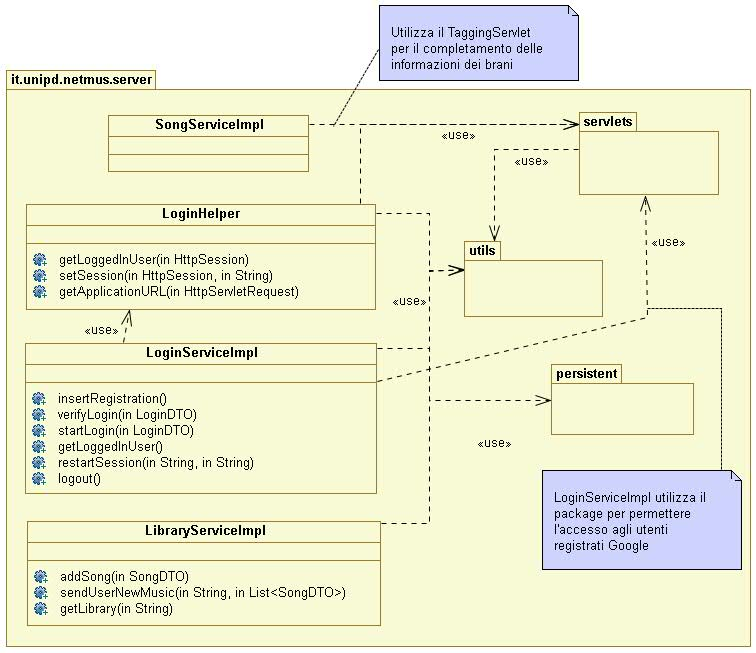
\includegraphics[width=15cm]{img/DP/classes_server.png}
\caption{Diagramma UML delle classi che descrive le dipendenze
fondamentali presenti all'interno del package
\emph{it.unipd.netmus.server}.}
\end{figure}


\subsection*{Requisiti obbligatori soddisfatti}
\begin{itemize}
	\item C1FN-1 WEB Application NetMus
	\item C1VN-1.11 Deve utilizzare il cloud computing
	\item C1VN-1.12 Deve utilizzare tecnologie GAE e GWT
	\item C1QN-2.6 Manutenibilit\`a
\end{itemize}
\subsection*{Requisiti desiderabili e opzionali soddisfatti}
\begin{itemize}
    \item Nessuno
\end{itemize}
\subsection*{Tipo, obiettivo e funzione del componente} % LASCIARE WARNING
Questo package racchiude tutte le classi che collaborano al fine di gestire la
\underline{business logic} del sistema, ovvero tutte quelle operazioni che
potranno essere compiute sui dati raccolti e che quindi interagiscono pesantemente con il
DataStore.  
\subsection*{Attivit\`a svolte e dati trattati}
Le attivit\`a svolte dalle sue classi verranno qui di seguito descritte.

\subsection{Classe SongsServiceImpl}
\subsubsection*{Requisiti obbligatori soddisfatti}
\begin{itemize}
    \item C1QN-1.6 Scalabilit\`a
\end{itemize}
\subsubsection*{Requisiti desiderabili e opzionali soddisfatti}
\begin{itemize}
    \item C1FD-1.1.4 Visualizza player YouTube
    \item C1FD-1.3 Personalizzazione del catalogo
    \item C1FD-1.3.1 Cancellazione brano
    \item C1FO-1.3.4 Ranking brani
    \item C1FD-1.5 Riproduzione tracce in streaming
    \item C1QD-1.5.1 Ottimizzazione della ricerca su YouTube
\end{itemize}
\subsubsection*{Tipo, obiettivo e funzione del componente}
Questa classe corrisponde all'implementazione del \co{SongsService} (di
\emph{client}) ed estende la classe \co{RemoteServiceServlet}. I metodi statici
qui definiti permettono le operazioni basilari sulle canzoni presenti nel
datastore. Le uniche eccezioni che possono causare il fallimento di queste
operazioni sono gli errori di stato del DataStore \co{IllegalStateException} che
verranno gestire tramite il callback nei metodi di \co{ProfileActivity}.
\subsubsection*{Attivit\`a svolte e
dati trattati} Implementa le funzionalit\`a di modifica e
cancellazione di un brano presente nel DataStore. Queste
operazioni agiscono su canzoni condivise da molti utenti e saranno
quindi utilizzate solo dove strettamente necessario. Ogni metodo ha tra gli
input l'username dell'utente che richiede l'operazione.
\begin{longtable}{|p{0.45\textwidth}|p{0.45\textwidth}|}
\hline
\rowcolor{orange} \bo{Metodo} & \bo{Descrizione} \\
\hline
\endhead
\hline
\multicolumn{2}{|c|}{\textit{continua alla pagina successiva}}\\
\hline
\endfoot
\endlastfoot
+ rateSong(in String,in SongSummaryDTO,in int): double & Assegna la
votazione compresa tra 1 e 5 alla canzone specificata dal
\co{SongSummaryDTO}. Dopo aver aggiornato i campi relativi di \co{Song} nel
DataStore ritorna il valore \emph{double} che rappresenta la nuova media
tra tutte le votazione effettuate su quella canzone.\\\hline 
+ editSong(in String,in String,in String,in String): boolean & Questo
metodo permette di assegnare una nuova chiave primaria ad una canzone
variando almeno uno tra gli attributi \emph{title}, \emph{artist} e
\emph{album} trasformandola di fatto in un altro brano nel DataStore.
Sar\`a possibile invocare questo metodo solamente su canzone le cui
informazioni che formano la chiave primaria sono incomplete.\\\hline 
+ deleteSong(in String,in String,in String,in String): boolean & Rimuove
la canzone dalla libreria dell'utente. Le canzoni rimosse rimangono nel
DataStore poich\'e potrebbero contenere informazioni utili per
inserimenti futuri.\\\hline
+ getSongDTO(in SongSummaryDTO): SongDTO & Carica dal Datastore le
informazioni complete rigurdanti la canzone data in input. In questo
metodo, se non ancora presenti in Datastore o in cache, vengono cercate
su servizi esterni le copertine di Last.fm ed i video YouTube.\\\hline
+ getCoverImage(in SongSummaryDTO): String & Carica dal Datastore o da Last.fm
la copertina relativa al brano in input. Per fare ci\`o utilizza la classe di
persistenza \co{Album}. \\\hline 
\caption{Metodi di SongServiceImpl}
\end{longtable}

\newpage
\subsection{Classe UsersServiceImpl}
\subsubsection*{Requisiti obbligatori soddisfatti}
\begin{itemize}
    \item C1FN-1.4 Gestione profilo personale
    \item C1FN-1.4.1 Modifica informazioni personali
    \item C1FN-1.4.2 Cambio password
    \item C1FN-1.4.3 Cancellazione del proprio account
    \item C1QN-1.6 Scalabilit\`a
\end{itemize}
\subsubsection*{Requisiti desiderabili e opzionali soddisfatti}
\begin{itemize}
    \item C1FD-1.3 Personalizzazione del catalogo
    \item C1FD-1.7 Interazione con altri utenti
    \item C1FD-1.7.1 Visualizzazione altri profili
\end{itemize}
\subsubsection*{Tipo, obiettivo e funzione del componente}
Questa classe corrisponde all'implementazione del \co{UsersService} (di
\emph{client}) ed estende la classe \co{RemoteServiceServlet}. Fornisce i metodi
statici che implementano le funzionalit\`a relative alla gestione del proprio
profilo utente.
\subsubsection*{Attivit\`a svolte e dati trattati} I metodi qui implementati
forniscono le funzionalit\`a di base quali la ricerca, la modifica e la
cancellazione di un utente di NetMus ma anche la ricerca di utenti affini.
\begin{longtable}{|p{0.45\textwidth}|p{0.45\textwidth}|}
\hline
\rowcolor{orange} \bo{Metodo} & \bo{Descrizione} \\
\hline
\endhead
\hline
\multicolumn{2}{|c|}{\textit{continua alla pagina successiva}}\\
\hline
\endfoot
\endlastfoot
+ loadProfile(in String): UserCompleteDTO  & Trova nel DataStore
l'utente a cui corrisponde l'username dato in input e ne ritorna le
informazioni incapsulate in un DTO. Gli utenti di cui viene richiesto il
caricamento devono essere presenti nel DataStore.\\\hline 
+ editProfile(in String,in UserCompleteDTO): boolean & Salva nell'
\co{UserAccount} del DataStore i dati presenti nell' \co{UserCompleteDTO} dato
in input sovrascrivendo le informazioni precedenti. \`E previsto qui anche il
cambio della password. \\\hline
+ deleteProfile(in String): boolean & Cancella irreversibilmente l'utente e
tutte le sue informazioni dal DataStore e conseguentemente lo reindirizza alla
pagina iniziale di login. Le canzoni che facevano parte del catalogo non
vengono cancellate. \\\hline
+ findSimilarUser(in String): List\textless UserDTO\textgreater & Cerca
nel DataStore i nomi degli utenti il cui catalogo ha propriet\`a simili
a quello dato in input. I criteri di somiglianza sono dati dall'artista
pi\`u ricorrente ed il genere pi\`u ascoltato. \\\hline
\caption{Metodi di UserServiceImpl}
\end{longtable}

\subsection{Classe LoginServiceImpl}
\subsubsection*{Requisiti obbligatori soddisfatti}
\begin{itemize}
    \item C1FN-1.2 Registrazione
    \item C1QN-1.6 Scalabilit\`a
\end{itemize}
\subsubsection*{Requisiti desiderabili e opzionali soddisfatti}
\begin{itemize}
    \item C1FO-1.2.1 Pagina login indipendente
\end{itemize}
\subsubsection*{Tipo, obiettivo e funzione del componente}
Questa classe corrisponde all'implementazione del \co{LoginService} (di
\emph{client}) ed estende la classe \co{RemoteServiceServlet}. Comprende i
servizi di autenticazione del sistema quali l'inserimento di una nuova
registrazione e la verifica dei dati di login. Una parte cospicua e molto
importante di questa classe \`e rappresentata dalla gestione delle sessioni e
dei cookie.
\subsubsection*{Attivit\`a svolte e dati trattati} Implementa la parte server
delle procedure di login come la verifica della correttezza della password e
l'adeguata impostazione delle sessioni HTTP.
\begin{longtable}{|p{0.4\textwidth}|p{0.4\textwidth}|}
\hline
\rowcolor{orange} \bo{Metodo} & \bo{Descrizione} \\
\hline
\endhead
\hline
\multicolumn{2}{|c|}{\textit{continua alla pagina successiva}}\\
\hline
\endfoot
\endlastfoot
+ insertRegistration(LoginDTO) & Inserisce i dati di login
relativi alla registrazione di un nuovo utente nel database. Pu\`o
lanciare eccezioni di tipo \textless= \co{RegistrationException} in caso vi
siano problemi nell'inserimento.\\\hline 
+ verifyLogin(LoginDTO) & Metodo
fondamentale per l'autenticazione che confronta i dati in input con quelli
presenti nel database per verificare se il login \`e valido. Pu\`o
lanciare eccezioni di tipo \textless= \co{LoginException} in caso il controllo
non vada a buon fine.\\\hline 
+ startLogin(LoginDTO) & Racchiude tutte i passi di autenticazione
dell'utente. Utilizza \co{verifyLogin} e si occupa di iniziare la sessione
dell'utente che si \`e autenticato aggiornando anche l'attributo
\co{lastLogin} in \co{UserAccount}.\\\hline 
+ getLoggedInUserDTO():
UserSummaryDTO & Esegue una ricerca della sessione corrente utilizzando i metodi
di \co{LoginHelper} e ritorna, se presenti, le informazioni di base
(\co{UserSummaryDTO}) dell'utente loggato\\\hline 
+ logout() & Invalida l'autenticazione dell'utente che viene rimandato alla pagina di login.\\\hline
+ restartSession(in String,in String): String & Recupera un eventuale
sessione salvata nei cookie controllandone la validit\`a per l'utente
dato in input. Questa funzionalit\`a non \`e valida per gli utenti
Google dei quali non viene gestito un cookie.\\\hline
\caption{Metodi di LoginServiceImpl}
\end{longtable}


\subsection{Classe LibraryServiceImpl}
\subsubsection*{Requisiti obbligatori soddisfatti}
\begin{itemize}
    \item C1QN-1.6 Scalabilit\`a
    \item C1FN-1.9 Ricezione ed elaborazione dei brani
    \item C1FN-1.9.1 Controllo di validit\`a dei dati
\end{itemize}
\subsubsection*{Requisiti desiderabili e opzionali soddisfatti}
\begin{itemize}
    \item C1FD-1.3 Personalizzazione del catalogo
    \item C1FO-1.3.3 Creazione playlist
    \item C1FO-1.3.4 Ranking brani
    \item C1FD-1.8 Elaborazione dati utente
    \item C1FO-1.8.1 Esportazione PDF
    \item C1FO-1.9.3 Completamento info da servizio esterno
\end{itemize}
\subsubsection*{Tipo, obiettivo e funzione del componente}
Questa classe corrisponde all'implementazione del \co{LibraryService} (di
\emph{client}) ed estende la classe \co{RemoteServiceServlet}. Si occupa di
fornire tutti i metodi necessari all'inserimento, lettura e modifica dei dati
nel DataStore relativi ad un catalogo musicale. Un
metodo di fondamentale importanza \`e
\emph{sendUserNewMusic} che gestisce l'inserimento di
una lista di canzoni singolarmente nel DataStore e nella
libreria.
\subsubsection*{Attivit\`a svolte e dati trattati} Implementa tutte le
attivit\`a necessarie alla gestione del catalogo musicale. Vengono qui definiti
i metodi di interazione con le Playlist e con il sistema di rating dei brani.
\begin{longtable}{|p{0.4\textwidth}|p{0.4\textwidth}|}
\hline
\rowcolor{orange} \bo{Metodo} & \bo{Descrizione} \\
\hline
\endhead
\hline
\multicolumn{2}{|c|}{\textit{continua alla pagina successiva}}\\
\hline
\endfoot
\endlastfoot
+ sendUserNewMusic(in String,in List\textless SongDTO\textgreater) &
Salva o aggiorna nel DataStore tutte le canzoni passate in input e se
possiedono sufficienti informazioni le inserisce nella libreria
dell'utente.\\\hline 
+ addPlaylist(in String,in String): boolean & Aggiunge una nuova
playlist vuota al catalogo dell'utente con il nome dato in input.
Ritorna \emph{true} se l'operazione ha successo.\\\hline 
+ removePlaylist(in String,in String): boolean & Cancella la playlist il
cui nome \`e dato in input dal catalogo. Ritorna \emph{true} se l'operazione ha
successo.\\\hline
+ getPlaylist(in String,in String): List\textless SongSummaryDTO\textgreater &
Ritorna la lista ordinate delle canzoni in forma di \co{SongSummaryDTO} che
appartengono alla playlist.Ritorna \emph{true} se l'operazione ha
successo.\\\hline
+ addSongToPlaylist(in String,in String,in String): boolean & Aggiunge
la canzone con l'id dato in input in coda alla playlist specificata. Ritorna \emph{true} se l'operazione ha
successo.\\\hline
+ moveSongInPlaylist(in String,in String,in int, in int): boolean &
Sposta la canzone all'indice dato in input nel primo attributo INT
all'indice specificato nel secondo, se questi indici sono validi
relativamente alla dimensione della playlist. Ritorna \emph{true} se l'operazione ha
successo.\\\hline 
+ removeSongFromPlaylist(in String,in String,in String): boolean & Rimuove
la canzone con l'id dato in input dalla playlist specificata.Ritorna \emph{true}
se l'operazione ha successo.\\\hline
+ loadPreferredArtists(in String): List\textless String\textgreater &
Calcola e ritorna l'artista pi\`u ricorrente all'interno delle canzoni
del catalogo dell'utente specificato. \\\hline
+ loadPreferredGenres(in String): List\textless String\textgreater & Calcola e
ritorna il genere pi\`u ricorrente all'interno delle canzoni del catalogo
dell'utente specificato. \\\hline
+ loadMostPopularSong(in String): String & Ritorna l'id della canzone condivisa
dal maggior numero di utenti che fa parte del catalogo.\\\hline
+ storeStatistics(in String, in String, in String, in String) & Salva
nel \co{MusicLibrary} persitente le statistiche relative al catalogo
calcolate nel client.\\\hline
+ generateDoc(in String): String & Questo metodo si occupa dell'intera
generazione del Google Doc dell'utente dato in input. La creazione
consiste nel creare il modello HTML del documento generandone
al momento i contenuti tramite le libreria \emph{velocity} e inserendoli poi in
un modello standard in \emph{template.mv}. Successivamente viene invocato il
metodo \co{createNewDocument} di \co{GdataManager} per la generazione del Doc
dal modello HTML. Ritorna l'indirizzo al documento. \\\hline
- check\_list(in List\textless String\textgreater, in String): int &
Funzione che aggiunge una stringa ad una lista verificandone
l'unicit\`a e ritorna 1 se ha succeso, viene utilizzata all'interno di
\co{GenerateDoc}.\\\hline

\caption{Metodi di LibraryServiceImpl}
\end{longtable}

\subsection{Classe LoginHelper}
\subsubsection*{Requisiti obbligatori soddisfatti}
\begin{itemize}
    \item C1FN-1.2 Registrazione
\end{itemize}
\subsubsection*{Requisiti desiderabili e opzionali soddisfatti}
\begin{itemize}
    \item C1FO-1.2.1 Pagina login indipendente
\end{itemize}
\subsubsection*{Tipo, obiettivo e funzione del componente}
La classe \co{LoginHelper} offre funzionalit\`a statiche
per gestire le sessioni HTML, utili a\\ \co{LoginServiceImpl} ed a
\emph{servlet}.
\subsubsection*{Attivit\`a svolte e dati trattati}
Questa classe ha il compito esclusivo di interagire con le
sessioni HTML, deve quindi occuparsi di reperire i dati utili
dalla sessione corrente e di impostarne una nuova. Fornisce inoltre il
controllo necessario al filtro \co{LoginFilter} per verificare se
l'utente che accede ad una pagina \`e gi\`a loggato oppure no.
\begin{longtable}{|p{0.4\textwidth}|p{0.4\textwidth}|}
\hline
\rowcolor{orange} \bo{Metodo} & \bo{Descrizione} \\
\hline
\endhead
\hline
\multicolumn{2}{|c|}{\textit{continua alla pagina successiva}}\\
\hline
\endfoot
\endlastfoot
+ getLoggedInUser(HttpSession session): String \emph{static} & Legge dal
database le informazioni relative all'utente specificato nella \co{HttpSession}
e ne restituisce l'username.\\\hline
+ getApplicationURL(in HttpServletRequest): String \emph{static} &
Restituisce l'URL attuale dell'applicazione, anche nel caso sia
eseguendo in development mode.\\\hline
+ setSession(in HttpSession,in String)
\emph{static} & Imposta una nuova sessione per l'utente in input.\\\hline
+ isDevelopment(in HttpServletRequest): boolean \emph{static} & Ritorna
\emph{true} solamente se l'applicazione sta eseguendo in development
mode altrimenti ritorna \emph{false}.\\\hline
\caption{Metodi di LoginHelper}
\end{longtable}


\newpage
\section{Package server.persistent} % LASCIARE WARNING

\begin{figure}[!h]
  \centering
  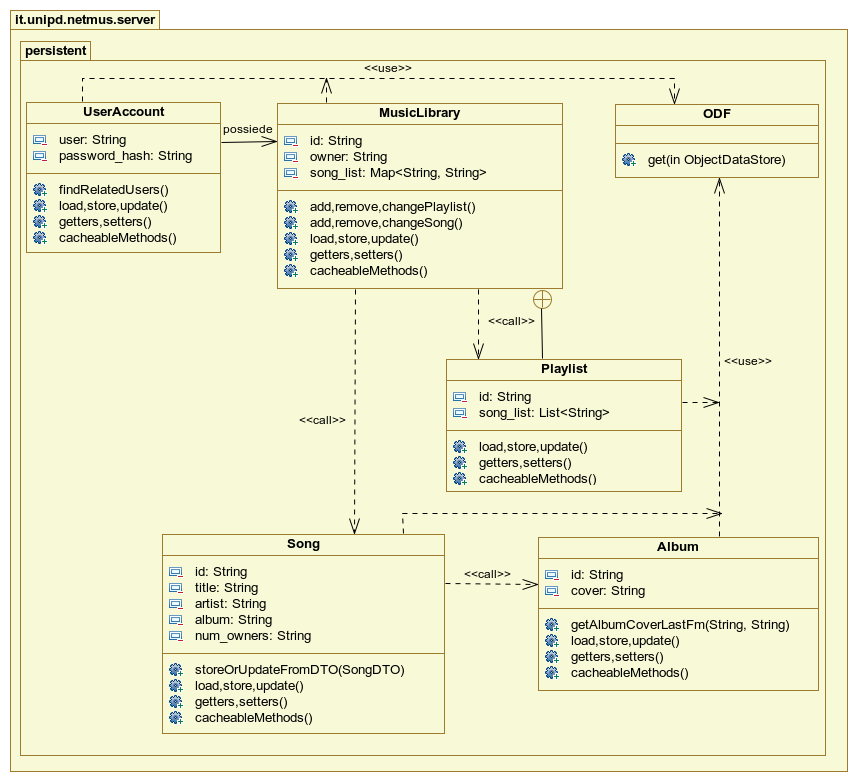
\includegraphics[width=17cm]{img/DP/classes_server_persistent.png}
\caption{Diagramma UML delle classi che descrive le dipendenze
fondamentali presenti all'interno del package
\emph{it.unipd.netmus.server.persistent}.}
\end{figure}


\subsection*{Requisiti obbligatori soddisfatti}
\begin{itemize}
    \item C1FN-1 Web Application NetMus
    \item C1QN-1.6 Scalabilit\`a
    \item C1QN-1.6.2 Scalabilit\`a massa di utenza
    \item C1FN-1.9.1 Controllo di validit\`a dei dati
	\item C1FN-1.9.5 Inserimento nel Database
	\item C1QN-1.9.6 Gestione concorrenza
	\item C1VN-1.11 Deve utilizzare il cloud computing
	\item C1VN-1.12 Deve utilizzare tecnologie GAE e GWT
	\item C1FN-1.13 Gestione Database
	\item C1VN-1.13.1 Deve utilizzare Google DataStore
	\item C1QN-2.6 Manutenibilit\`a
\end{itemize}
\subsection*{Requisiti desiderabili e opzionali soddisfatti}
\begin{itemize}
    \item Nessuno
\end{itemize}
\subsection*{Tipo, obiettivo e funzione del componente}
Il package \emph{server.persistent} contiene le classi di persistenza che
implementano il \underline{design pattern} \emph{Data Access Object (DAO)} che
hanno lo scopo di interfacciare il sistema con il database nascondendo cos\`i ogni
dettaglio sulla struttura del database all'esterno.\
I DAO sono implementati con l'utilizzo del framework \emph{Twig-persist}
introdotto nel capitolo 3, la notazione utilizzata contiene alcuni elementi
introdotti dal framework per gestirne la configurazione: 
\begin{itemize}
  \item \bo{@Id}: L'attributo definito con questa annotazione rappresenta la
  chiave identificativa dell'entit\`a che deve essere unica all'interno del
  DataStore. Definirla nel DAO ci permette di gestire questa chiave a nostro
  piacimento.
  \item \bo{@Index}: Serve ad indicizzare un particolare attributo poich\'e di
  default il datastore che viene utilizzato indicizza solo la chiave. Questa
  annotazione deve essere utilizzata su tutti gli attributi che sono soggetti a
  ricerca o ordinamento.
  \item \bo{@Child}: Assegna la relazione di ``figlio'' ad un attributo
  che ha come tipo un'altra entit\`a del DataStore, in particolare nella chiave
  dell'entit\`a figlia sar\`a presente anche quella del padre in modo che sia
  associata a nessun'altro oggetto.
  \item \bo{@Parent}: Come descritto sopra viene utilizzata per convenienza
  insieme all'annotazione @Child per avere un riferimento all'entit\`a padre
  nell'entit\`a figlia.
  \item \bo{@Type(Type.class)}: Questa annotazione dice esplicitamente alla
  classe di twig-persist \co{ObjectFieldTraslator} come tradurre il tipo dell'attributo
  nel tipo effettivo nel DataStore.
\end{itemize}
Per avere l'istanza del DataStore su cui lavorare si
utilizza la classe con visibilit\`a \emph{package} \co{ODF}. \\
Le classi di persitenza presenti in questo package, inoltre, implementano le
interfacce \co{Serializable} e \co{Cacheable} poich\'e sono gestite anche come
entit\`a della App Engine Memcache. 
\subsubsection*{Businness logic interna} Nonostante il design pattern DAO non lo
preveda vengono implementate alcune componenti di businness logic all'interno
delle classi di persistenza. Questo va leggermente a scapito della riusabilit\`a
ma viene giustificato dal fatto che la logica di businness qui trattata \`e
molto semplice e strettamente legata all'implmentazione interna dei DAO. Una
separazione delle cose genererebbe confusione all'interno del progetto
raddoppiando i file di questo package. Vi \`e un'eccezione per quanto
riguarda la classe \co{MusicLibrary} che \`e stata
progettata come vero e proprio ``businnes object'' ed \`e la causa
dell'incongruenza con il pattern DAO. Ci \`e estremamente utile per\`o per
alleggerire il numero di campi dati e metodi da \co{UserAccount} e mantiene
dunque questa natura ibrida tra classe di persistenza e businness object.

\subsection*{Attivit\`a svolte e dati trattati} Le classi DAO
gestiscono i dati del sistema garantendone la persistenza e si occupano anche di implementare la parte logica di salvataggio, recupero e
relazione dei dati con utilizzo della Memcache. Nel caso di NetMus \`e
un'attivit\`a molto delicata poich\'e il \underline{database} utilizzato \`e \underline{non-relazionale}.

\subsection{Classe ODF (Singleton)}
\subsubsection*{Requisiti obbligatori soddisfatti}
\begin{itemize}
    \item C1QN-1.6 Scalabilit\`a
    \item C1QN-1.6.2 Scalabilit\`a massa di utenza
    \item C1QN-1.9.6 Gestione concorrenza
    \item C1FN-1.13 Gestione Database
    \item C1VN-1.13.1 Deve utilizzare Google DataStore
\end{itemize}
\subsubsection*{Requisiti desiderabili e opzionali soddisfatti}
\begin{itemize}
    \item Nessuno
\end{itemize}
\subsubsection*{Tipo, obiettivo e funzione del componente}
\co{ODF} (Object DataStore Factory) \`e una classe \emph{final} che segue il
pattern Singleton illustrato in \emph{SpecificaTecnica v3.0}. Ha la funzione di creare un'unica istanza del
\co{ObjectDataStore} fornito dal framework twig-persist e di restituirla a
qualunque oggetto la richieda. Quest'ultimo da la possibilit\`a di interagire
con il DataStore, inviando \underline{query}, memorizzando oggetti
\emph{persistent} o richiedendo liste di oggetti tramite semplici metodi.
L'oggetto datastore restituito \`e di tipo \co{AnnotationObjectDatastore} che di
default salva gli attributi degli oggetti persistenti in modo non indicizzato
rendendo il datastore pi\`u rapido.\\ Questa classe \`e visibile solamente
all'interno del package \emph{persistent}.
\subsubsection*{Attivit\`a svolte e dati trattati}
Crea un'unica istanza di \co{ObjectDataStore} e tramite un metodo
statico \emph{get()} la passa alle classi, in maniera di dargli la possibilit\`a
di usare il database.
\begin{longtable}{|p{0.4\textwidth}|p{0.4\textwidth}|}
\hline
\rowcolor{orange} \bo{Metodo} & \bo{Descrizione} \\
\hline
\endhead
\hline
\multicolumn{2}{|c|}{\textit{continua alla pagina successiva}}\\
\hline
\endfoot
\endlastfoot
- datastore\_istance: DataStoreObject \emph{static, final} & Unica istanza dell'
\co{ObjectDataStore} che viene inizializzata alla creazione della classe
con un \co{AnnotationObjectDataStore}.\\\hline
\caption{Campi dati di ODF}
\end{longtable}
\begin{longtable}{|p{0.4\textwidth}|p{0.4\textwidth}|}
\hline
\rowcolor{orange} \bo{Metodo} & \bo{Descrizione} \\
\hline
\endhead
\hline
\multicolumn{2}{|c|}{\textit{continua alla pagina successiva}}\\
\hline
\endfoot
\endlastfoot
+ get(): ObjectDataStore \emph{static} & Ritorna l'istanza
dell' \co{ObjectDataStore}.\\\hline
\caption{Metodi dati di ODF}
\end{longtable}


\subsection{Classe UserAccount}
\subsubsection*{Requisiti obbligatori soddisfatti}
\begin{itemize}
    \item C1FN-1.2 Registrazione a NetMus
    \item C1FN-1.4 Gestione profilo personale
    \item C1FN-1.4.1 Modifica informazioni personali
    \item C1FN-1.4.2 Cambio password
    \item C1FN-1.4.3 Cancellazione del proprio account
    \item C1QN-1.6 Scalabilit\`a
    \item C1QN-1.6.2 Scalabilit\`a massa di utenza
    \item C1FN-1.9.1 Controllo di validit\`a dei dati
    \item C1FN-1.13 Gestione Database
\end{itemize}
\subsubsection*{Requisiti desiderabili e opzionali soddisfatti}
\begin{itemize}
    \item C1FD-1.3 Personalizzazione del catalogo
    \item C1FD-1.7 Interazione con altri utenti
    \item C1FD-1.7.1 Visualizzazione altri profili
\end{itemize}
\subsubsection*{Tipo, obiettivo e funzione del componente}
\co{UserAccount} utilizza il design pattern DAO poich\'e contiene tutte le
informazioni relative ad un utente cos\`i come viene salvato all'interno del
Datastore. La classe \`e implementata come \underline{POJO} poich\'e
twig-persist lo supporta senza bisogno di configurazioni aggiuntive. Vengono usate solamente
le annotazioni \emph{@Key} e \emph{@Index} per gestire l'indicizzazione
degli oggetti nel datastore. La sua funzione di \co{load} \`e particolarmente
importante poich\'e carica dalla cache o dal Datastore tutte le informazioni
rigurdanti l'utente ed il suo catalogo. Estende le interfacce \co{Serializable}
e \co{Cacheable} per gestirne la scrittura e la
lettura in Memcache.
\subsubsection*{Metodo load}
\begin{figure}[!h]
  \centering
  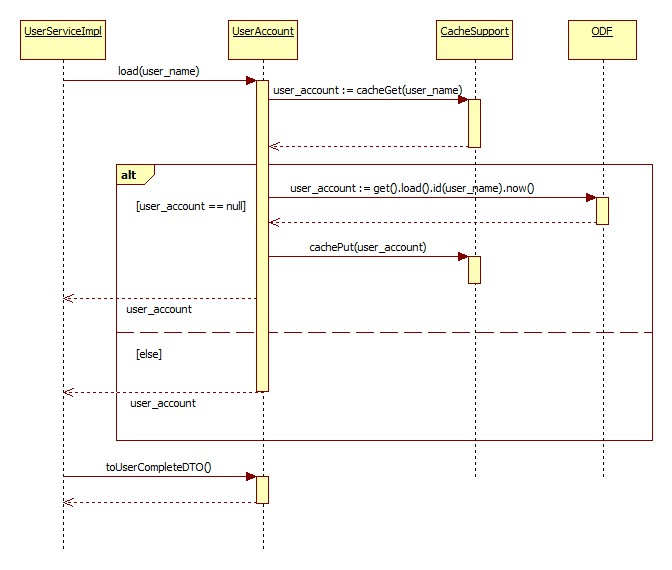
\includegraphics[width=17cm]{img/DP/load_user.jpg}
\caption{Diagramma UML di sequenza che descrive il procedimento di lettura
delle informazioni riguardanti un utente lato server.}
\end{figure}
Il metodo \co{load()} che viene invocato tramite chimate RPC di tipo
\co{UserSerivice} \`e molto dispendioso come tempo di calcolo poich\'e si occupa
di caricare l'intera libreria dell'utente che, in alcuni casi, verr\`a
anche trasformata in DTO e spedita al client. Va considerato anche che questo
metodo viene usato moltissimo dei Service dato che i parametri in entrata sono
sempre degli username (String) e da questi spetta al server il compito di
ricavarne l'oggetto persistente. Per gestire nel modo pi\`u approrpiato il
problema si \`e deciso di gestire la Memcache lato server che permette la
lettura degli oggetti con una velocit\`a 5 volte superiore a quella del
Datastore. Questa sequenza di operazioni, progettata seguendo il Memcache
pattern di App Engine, viene utilizzata anche per le altre classi del package
persitent, anche se con un vantaggio meno evidente.
\subsubsection*{Attivit\`a svolte e dati trattati} Gestisce la
logica di persistenza di tutti i dati relativi ad un utente del sistema NetMus. Gestisce inoltre alcuni elementi di businness logic strettamente legati a questa entit\`a come la ricerca di particolari utenti all'interno del Datastore.
\begin{longtable}{|p{0.4\textwidth}|p{0.4\textwidth}|}
\hline
\rowcolor{orange} \bo{Attributo} & \bo{Descrizione} \\
\hline
\endhead
\hline
\multicolumn{2}{|c|}{\textit{continua alla pagina successiva}}\\
\hline
\endfoot
\endlastfoot
 - user: String \emph{@Id} & Rappresenta il nome di login unico
 dell'utente e nello stesso tempo la sua e-mail (valida). Viene
 impiegato come chiave dell'entit\`a nel DataStore.\\\hline
 - password\_hash: String & Contiene l'hash della password dell'utente ottenuto
  utilizzando l'algoritmo \underline{BCrypt}.\\\hline
 - nick\_name: String & Nickname di un utente visibile anche agli
 altri.\\\hline - first\_name: String & Nome proprio dell'utente.\\\hline
 - last\_name: String & Cognome dell'utente.\\\hline
 - gender: char & Sesso, sono validi i valori 'F' (femmina) e 'M'
 (maschio).\\\hline
 - nationality: String & Nazione di provenienza dell'utente.\\\hline
 - about\_me: String \emph{@Type(Text.class)} & Informazioni aggiuntive su
 di se inserite dall'utente.\\\hline
 - last\_session\_id: String \emph{@Index} & Codice identificativo dell'ultima
 sessione di autenticazione dell'utente. Campo necessario per l'utilizzo dei
 cookies per mantenere la sessione anche quando viene chiuso il browser.\\\hline
 - is\_google\_user: boolean & Flag che indica se l'utente accede al sistema
 tramite l'autenticazione di Google. \\\hline
 - is\_public\_profile: boolean & Flag che
 indica se il profilo dell'utente \`e visibile ad altri utenti oppure no.\\\hline 
 - allowed\_users: List\textless String\textgreater & Lista degli username
 degli utenti che possono visualizzare questo profilo ed il relativo catalogo.\\\hline
 - music\_library:
 MusicLibrary \emph{@Child} & Intera libreria musicale dell'utente, non sempre verr\`a caricata dal DataStore insieme alle informazioni dell'utente.\\\hline
\caption{Campi dati di UserAccount}
\end{longtable}
\begin{longtable}{|p{0.4\textwidth}|p{0.4\textwidth}|}
\hline
\rowcolor{orange} \bo{Metodo} & \bo{Descrizione} \\
\hline
\endhead
\hline
\multicolumn{2}{|c|}{\textit{continua alla pagina successiva}}\\
\hline
\endfoot
\endlastfoot
 + store() & Inserisce nel database per la prima volta l'utente. Se
 esiste gi\`a un utente con lo stesso id lancia un'eccezione di tipo
 \co{IllegalStateException} \\\hline
 + update() & Aggiorna o inserisce i dati dell'utente nel DataStore e
 nella Memcache.\\\hline
  + load(in String): UserAccount
 \emph{static}& Cerca nella Memcache e successivamente nel database e
 restituisce tutti i dati relativi ad un username/e-mail dato come input. \\\hline 
 + deleteUser(in UserAccount) \emph{static} & Rimuove completamente dal database
 l'utente dato in input. Le canzoni relative a quell'utente vengono per\`o
 mantenute per non perdere informazioni importanti. \\\hline
 + toLoginDTO(): LoginDTO &
 Genera un oggetto LoginDTO contenente le informazioni di autenticazione dell'utente.\\\hline
 + toUserDTO(): UserDTO & Genera un oggetto UserSummaryDTO
contenente buona parte delle informazioni riguardanti l'utente.\\\hline
 + toUserCompleteDTO(): UserCompleteDTO & Genera un oggetto UserSummaryDTO
contenente tutte le informazioni riguardanti l'utente.\\\hline
 + findSessionUser(in String): UserAccount \emph{static} & Cerca nel database e
 ritorna i dati relativi ad un utente che come lastSessionId ha l'id si sessione
 HTTP dato in input.\\\hline
 + findRelatedUsers(): List\textless String\textgreater & Ritorna la lista (con
 un massimo di 20 utenti) degli utenti che hanno lo stesso artista preferito
 dell'utente.\\\hline
 + cacheableMethods() & Implementazione adeguata dei metodi ereditati
 dall'interfaccia \co{Cacheable}.\\\hline
 + getters() & Tutti gli attributi privati di questa
 classe hanno i relativi metodi \emph{get}.\\\hline 
 + setters() & Tutti gli attributi privati di questa classe hanno i relativi
 metodi \emph{set}. Tutti questi metodi si occupano anche di chiamare
 \co{update()} per aggiornare i dati del DataStore.\\\hline
 \caption{Metodi di UserAccount}
\end{longtable}


\subsection{Classe MusicLibrary}
\subsubsection*{Requisiti obbligatori soddisfatti}
\begin{itemize}
	\item C1QN-1.6 Scalabilit\`a
	\item C1QN-1.6.2 Scalabilit\`a massa di utenza
	\item C1FN-1.9.1 Controllo di validit\`a dei dati
	\item C1FN-1.9.5 Inserimento nel Database
	\item C1FN-1.13 Gestione Database
\end{itemize}
\subsubsection*{Requisiti desiderabili e opzionali soddisfatti}
\begin{itemize}
    \item C1FD-1.3 Personalizzazione del catalogo
    \item C1FO-1.3.3 Creazione playlist 
    \item C1FO-1.3.4 Ranking brani
    \item C1FD-1.8 Elaborazione dati utente
    \item C1FO-1.8.1 Esportazione PDF
\end{itemize}
\subsubsection*{Tipo, obiettivo e funzione del componente} \co{MusicLibrary}
contiene tutte le informazioni relative ad un catalogo multimediale, ovvero
il proprietario, la lista delle canzoni, la lista delle playlist ed alcuni dati
statistici. La funzione principale per\`o \`e quella di fornire dei servizi comodi ed efficienti per la gestione del catalogo
stesso e le entit\`a interne ad esso associate.\\
La lista di brani \`e mantenuta
come mappa di codici identificativi (strighe) e punteggio associato
dall'utente alla canzone. Questo grantisce un'ottima efficenza grazie alla
conversione della mappa nel Datastore da parte del framework twig-persist.\\
Estende le interfacce \co{Serializable}
e \co{Cacheable} per gestirne la scrittura e la
lettura in Memcache.
\subsubsection*{Attivit\`a svolte e dati trattati} Gestisce la logica di
persistenza e le procedure di reperimento delle informazioni di tutti i dati
relativi ad un catalogo multimediale del sistema NetMus. Le attivit\`a svolte da
questa classe sono quindi moltissime tanto che potrebbe essere considerata una
classe di businness logic piuttosto che una classe di persistenza.
\begin{longtable}{|p{0.4\textwidth}|p{0.4\textwidth}|}
\hline
\rowcolor{orange} \bo{Attributo} & \bo{Descrizione} \\
\hline
\endhead
\hline
\multicolumn{2}{|c|}{\textit{continua alla pagina successiva}}\\
\hline
\endfoot
\endlastfoot
 - id: String \emph{@Id} & Id univoco della libreria, \`e generato a partire
 dall'utente che la possiede. \\\hline
 - owner: UserAccount \emph{@Id @Parent} & L'utente
 a cui \`e associata questa libreria. \\\hline
 - song\_list: Map\textless Striing, String\textgreater & Mappa che 
 contiene le canzoni con punteggio che fanno parte del catalogo. Il
 punteggio \`e salvato come stringa poich\'e la conversione di twig non
 supporta gli interi.\\\hline
 - preferred\_artist: String \emph{@Index} & Nome dell'artista pi\`u ricorrente
 nelle canzoni del catalogo.\\\hline 
 - most\_popular\_song: String \emph{@Index} & Canzone, o la prima delle, che
 l'utente ha valutato meglio.\\\hline 
 - most\_popular\_song\_for\_this\_user: String \emph{@Index} & Canzone, o la
 prima delle, che \`e stata valutata meglio tra tutti gli utenti di Netmus che la
 condividono.\\\hline 
 - playlists: List\textless Playlist\textgreater \emph{@Index} & Lista
 contenente tutte le playlist create per questo catalogo musicale.\\\hline
 - classe Playlist \emph{static} & Classe interna che rappresenta una sequenza
 di canzoni ordinate e fornisce i metodi per le operazioni basilari come
 la creazione, l'aggiornamento e la cancellazione di una playlist. Ogni oggetto
 di questa classe ha un id univoco, un nome ed una
 lista di canzoni non necessariamente diverse tra loro. \\\hline
 
 \\\hline
\caption{Campi dati di MusicLibrary}
\end{longtable}
\begin{longtable}{|p{0.4\textwidth}|p{0.4\textwidth}|}
\hline
\rowcolor{orange} \bo{Metodo} & \bo{Descrizione} \\
\hline
\endhead
\hline
\multicolumn{2}{|c|}{\textit{continua alla pagina successiva}}\\
\hline
\endfoot
\endlastfoot
 + store() & Inserisce nel database per la prima volta la libreria musicale. Se
 esiste gi\`a una libreria per quel dato utente utente lancia
 un'eccezione di tipo \co{IllegalStateException} \\\hline
 + update() & Aggiorna o inserisce i dati della libreria nel datastore
 e nella Memcache.\\\hline 
 \# deleteMusicLibrary(in MusicLibrary) \emph{static}
 & Rimuove completamente dal database la libreria data in input. Le canzoni
 relative a quella libraria vengono per\`o mantenute per non perdere
 informazioni importanti. \\\hline 
 + toMusicLibraryDTO(): MusicLibrarySummaryDTO & Genera un oggetto
 \co{MusicLibrarySummaryDTO} contenente le informazioni
 della libreria e quelle essenziali riguardanti le canzoni in essa
 contenute.\\\hline
 + addSong(in Song): boolean & Associa una canzone data in
 input alla libreria aggiungendola in coda. Ritorna \emph{true} se
 l'inserimento ha avuto successo, \emph{false} altrimenti.\\\hline 
 + removeSong(in Song): boolean & Rimuove una canzone data in input dalla
 libreria, la canzone rimossa rimane in database anche se non posseduta da alcun
 utente. Ritorna \emph{true} se
 la rimozione ha avuto successo, \emph{false} altrimenti.\\\hline 
 + allSongs(): List\textless Song\textgreater & Ritorna la lista ordinata di
 canzoni presenti nel catalogo.\\\hline
 + rateSong(in Song,in int) & Assegna il voto alla canzone dati in
 input. Il voto \`e personale dell'utente che possiede la libreria ed
 \`e unico, quindi sovrascrive la votazione precedente. Oltre ad aggiornare il
 voto del'utente in \co{MusicLibrary} questo metodo aggiorna anche la media
 totale dei voti in \co{Song}. \\\hline 
 + addPlaylist(in String): boolean & Aggiunge una nuova playlist vuota
 alla libreria con il nome dato in input.\\\hline 
 + removePlaylist(in String): boolean & Rimuove dalla libreria e
 cancella irreversibilmente la playlist il cui nome \`e dato in input.\\\hline
 - getPlaylist(in String): Playlist & Restituisce la playlist
 appartenete alla libreria richiesta.\\\hline 
 + getPlaylists(): List\textless String\textgreater & Ritorna la lista
 dei nomi di tutte le playlist appartenenti alla libreria.\\\hline 
 + getPlaylistSongs(in String): List\textless Song\textgreater & Ritorna
 la lista di tutte le canzoni appartenenti alla playlist il cui nome \`e
 dato in input.\\\hline 
 + getPlaylistSongNames(in String): List\textless Song\textgreater &
 Ritorna la dei codici delle canzoni appartenenti alla playlist il cui
 nome \`e dato in input.\\\hline 
 + addSongToPlaylist(in String, in String): boolean & Inserisce la
 canzone alla playlist date in input.\\\hline 
 + moveSongInPlaylist(in String,in int,in int) & Sposta nella playlist la
 canzone che si trova nella posizione indicata nel primo parametro int nella
 posizione specificata dal secondo. \\\hline 
 + removeSongFromPlaylist(in String,in String):boolean & Rimuove la
 canzone dalla playlist dati in input.\\\hline 
 + cacheableMethods() & Implementazione adeguata dei metodi ereditati
 dall'interfaccia \co{Cacheable}.\\\hline
 + getters() & Tutti gli attributi privati di questa classe hanno i relativi
 metodi \emph{get}.\\\hline 
 + setters() & Tutti gli attributi privati di questa classe hanno i relativi
 metodi \emph{set}. Tutti questi metodi si occupano anche di chiamare
 \co{update()} per aggiornare i dati del DataStore.\\\hline
 \emph{addSong()}.\\\hline  
\caption{Metodi di MusicLibrary}
\end{longtable}

\subsection{Classe Song}
\subsubsection*{Requisiti obbligatori soddisfatti}
\begin{itemize}
    \item C1QN-1.6 Scalabilit\`a
    \item C1QN-1.6.2 Scalabilit\`a massa di utenza
	\item C1FN-1.9 Ricezione ed elaborazione dei brani
	\item C1FN-1.9.1 Controllo di validit\`a dei dati
	\item C1FN-1.9.2 Completamento info da database interno
	\item C1QN-1.9.4 Identificazione dati ridondanti
	\item C1FN-1.9.5 Inserimento nel Database
	\item C1FN-1.13 Gestione Database
\end{itemize}
\subsubsection*{Requisiti desiderabili e opzionali soddisfatti}
\begin{itemize}
    \item C1FD-1.1.4 Visualizza player YouTube
    \item C1FD-1.3 Personalizzazione del catalogo
    \item C1FD-1.3.1 Cancellazione brano
    \item C1FO-1.3.4 Ranking brani
    \item C1FD-1.5 Riproduzione tracce in streaming
    \item C1FD-1.8 Elaborazione dati utente
    \item C1FO-1.9.3 Completamento info da servizio esterno
\end{itemize}
\subsubsection*{Tipo, obiettivo e funzione del componente} Contiene le
informazioni relative ad un brano musicale, in particolare ogni canzone \`e
identificata da una chiave univoca composta dal titolo, un separatore di
default, l'artista e l'album disposte nell'ordine titolo-sep-artista-sep-album
e i tre campi sono puliti da ogni carattere diverso dalle lettere dell'alfabeto
ed i numeri in modo da rendere la ricerca nel Datastore pi\`u efficace
possibile. Dei brani condivisi da pi\`u utenti viene salvata una sola copia per ottimizzare
la quantit\`a di spazio utilizzato.\\ 
La logica di salvataggio delle canzoni implementata prevede che nei tag estratti
sia presente almeno il titolo altrimenti il brano non verr\`a mantenuto nel
Datastore. 
Estende le interfacce \co{Serializable}
e \co{Cacheable} per gestirne la scrittura e la
lettura in Memcache.
\subsubsection*{Attivit\`a svolte e dati
trattati} Gestisce la logica di persistenza di tutti i dati relativi ad un brano musicale del
sistema NetMus. Le attivit\`a previste in questa classe non sono molte ma sono
fondamentali per la logica di funzionamento di Netmus.
\begin{longtable}{|p{0.4\textwidth}|p{0.4\textwidth}|}
\hline
\rowcolor{orange} \bo{Attributo} & \bo{Descrizione} \\
\hline
\endhead
\hline
\multicolumn{2}{|c|}{\textit{continua alla pagina successiva}}\\
\hline
\endfoot
\endlastfoot
 - id: String \emph{@Id} & Chiave univoca della canzone, \`e composta dal
 titolo, il separatore di default e l'artista. \\\hline 
 - title: String & Titolo del brano.\\\hline 
 - artist: String & Nome della band o del cantante autore
 della canzone.\\\hline 
 - genre: String & Genere musicale associato alla
 canzone.\\\hline 
 - num\_owners: int & Numero di utenti che possiedono la
 canzone nel proprio catalogo.\\\hline 
 - album:String & Album a cui appartiene il brano..\\\hline 
 - year: String & Anno di pubblicazione del brano.\\\hline 
 - composer: String & Nome del compositore della canzone.\\\hline
 - track\_number: String & Numero della canzone all'interno dell'album.\\\hline
 - rating: double & Media di tutti i voti assegnati dagli utenti a questa
 canzone.\\\hline
 - num\_ratings: int & Numero di voti effettuati su questa canzone. \\\hline
\caption{Campi dati di Song}
\end{longtable}
\begin{longtable}{|p{0.4\textwidth}|p{0.4\textwidth}|}
\hline
\rowcolor{orange} \bo{Metodo} & \bo{Descrizione} \\
\hline
\endhead
\hline
\multicolumn{2}{|c|}{\textit{continua alla pagina successiva}}\\
\hline
\endfoot
\endlastfoot
 + store() & Inserisce nella Memcache e nel database per la prima volta la
 canzone. Se esiste gi\`a un brano con lo stesso \co{id} lancia
 un'eccezione di tipo \co{IllegalStateException} \\\hline
 + update() & Aggiorna o inserisce i dati della canzone nel DataStore e
 nella Memcache.\\\hline 
 \# deleteSong(in Song) \emph{static} & Rimuove
 completamente dal database la canzone. \\\hline
 + load(in String): Song & Carica dalla Memcache o dal Datastore
 l'oggetto \co{Song} in cui id \`e dato in input.\\\hline
 + loadFromDTO(in SongSummaryDTO): Song & Carica dalla Memcache o dal Datastore
 l'oggetto \co{Song} le cui informazioni di base sono date in input con
 un \co{SongSummaryDTO}.\\\hline
 + toSongSummaryDTO(): SongSummaryDTO &
 Genera un oggetto \co{SongSummaryDTO} contenente le informazioni
 essenziali del brano.\\\hline
 + toSongDTO(): SongDTO &
 Genera un oggetto \co{SongDTO} contenente tutte le informazioni
 riguardanti la canzone.\\\hline 
 + storeOrUpdateFromDTO(in SongDTO): Song \emph{static} & Recupera le
 informazioni da un oggetto \co{SongDTO} e le salva nel modo pi\`u
 opportuno nel DataStore.\\\hline 
 + changeArtist(in String): Song & Modifica l'attributo \co{artist}
 inserendo, se valido, la stringa in input. Se la modifica trasforma la
 canzone in un brano gi\`a presente nel DataStore viene ritornato il
 brano gi\`a salvato.\\\hline
 + changeTitle(in String): Song & Modifica l'attributo \co{title}
 inserendo, se valido, la stringa in input. Se la modifica trasforma la
 canzone in un brano gi\`a presente nel DataStore viene ritornato il
 brano gi\`a salvato.\\\hline
 + changeAlbum(in String): Song & Modifica l'attributo \co{album}
 inserendo, se valido, la stringa in input. Se la modifica trasforma la
 canzone in un brano gi\`a presente nel DataStore viene ritornato il
 brano gi\`a salvato.\\\hline
 + addRate(in int): double & Aggiunge la votazione data in input
 alla canzone aggiornando nel modo appropriato gli attributi
 \emph{rating} e \emph{num\_ratings}. Questo metodo, poich\'e gli stessi dati
 possono essere acceduti concorrentemente, viene eseguito all'interno di una
 transazione. \\\hline
 + changeRate(in int,in int): double & Permette ad ogni utente di modificare
 la propria votazione su questo brano dando in input il voto precedente e
 quello nuovo. Questo metodo, poich\'e gli stessi dati possono essere acceduti
 concorrentemente, viene eseguito all'interno di una transazione. \\\hline 
 \# newOwner() & Incrementa il contatore dei possessori di questo brano, ha visibilit\`a package poich\'e la sua modifica deve avvenire solo all'interno della logica di persistenza nei DAO.\\\hline \# deleteOwner() & Decrementa il contatore dei possessori di questo brano, ha visibilit\`a package poich\'e la sua modifica deve avvenire solo
 all'interno della logica di persistenza nei DAO.\\\hline 
 + cacheableMethods() & Implementazione adeguata dei metodi ereditati
 dall'interfaccia \co{Cacheable}.\\\hline
 + getters() & Tutti gli attributi privati di questa classe hanno i relativi metodi \emph{get}.\\\hline 
 + setters() & Tutti gli attributi privati di questa classe hanno i relativi
 metodi. Tutti questi metodi si occupano anche di chiamare
 \co{update()} per aggiornare i dati del DataStore. \emph{set}.\\\hline
\caption{Metodi di Song}
\end{longtable}


\subsection{Classe Album}
\subsubsection*{Requisiti obbligatori soddisfatti}
\begin{itemize}
    \item C1QN-1.6 Scalabilit\`a
    \item C1QN-1.6.2 Scalabilit\`a massa di utenza
    \item C1FN-1.9 Ricezione ed elaborazione dei brani
    \item C1FN-1.9.2 Completamento info da database interno
    \item C1FN-1.9.5 Inserimento nel Database
    \item C1FN-1.13 Gestione Database
\end{itemize}
\subsubsection*{Requisiti desiderabili e opzionali soddisfatti}
\begin{itemize}
    \item C1FO-1.9.3 Completamento info da servizio esterno
\end{itemize}
\subsubsection*{Tipo, obiettivo e funzione del componente} Questa classe opera
come un contenitore per la lista degli album disponibili da cui gli altri
oggetti possono attingere. Fornisce inoltre la businness logic necessaria alla
ricerca esterna di copertine tramite le API di Last.fm ed alla ricerca interna
al Datastore.\\
Implementa le interfacce \co{Serializable} e \co{Cacheable} poich\'e viene gli
album vengono gestiti anche nella Memcache. 
\subsubsection*{Attivit\`a svolte e dati trattati} Ogni album \`e rappresentato
da una chiave univoca (\co{id}) e dal link alla copertina ad esso associata.
Questa classe ha lo scopo di mantenere nel Datastore tutte le copertine
ricercate su Last.fm in modo ordinato, minimizzando cos\`i le richieste esterne.
\begin{longtable}{|p{0.4\textwidth}|p{0.4\textwidth}|}
\hline
\rowcolor{orange} \bo{Attributo} & \bo{Descrizione} \\
\hline
\endhead
\hline
\multicolumn{2}{|c|}{\textit{continua alla pagina successiva}}\\
\hline
\endfoot
\endlastfoot
 - id: String \emph{@Id} & Chiave univoca assegnata ad un album, \`e generata a
 partire dal nome dell'album e dall'artista. \\\hline 
 - cover: String & Link all' immagine della copertina dell'album,
 l'immagine si trova su Last.fm.\\\hline
\caption{Campi dati di Album}
\end{longtable}
\begin{longtable}{|p{0.4\textwidth}|p{0.4\textwidth}|}
\hline
\rowcolor{orange} \bo{Metodo} & \bo{Descrizione} \\
\hline
\endhead
\hline
\multicolumn{2}{|c|}{\textit{continua alla pagina successiva}}\\
\hline
\endfoot
\endlastfoot
 + load(in String) \emph{static} & Legge dalla cache e, se non presente, dal
 Datastore l'album la cui chiave univoca \`e data in input. \\\hline
 + getAlbumCover(in String, in String): String \emph{static} & Ritorna
 il link alla copertina dell'album associato al nome e all'artista dati
 in input. Se l'album non \`e presente nel Datastore o se la copertina non
 \`e ancora stata ricercata su Last.fm viene ritornata la stringa vuota.\\\hline
 + storeNewAlbum(in String, in String): boolean \emph{static} & Salva
 nel Datastore l'album con il nome e l'artista dati in input. Ritorna
 \emph{false} nel caso in cui l'album specificato sia gi\`a presente.\\\hline
 + getAlbumCoverLastFm(in String, in String): String \emph{static} & Ritorna
 il link alla copertina dell'album associato al nome e all'artista dati
 in input. Se l'album non \`e presente nel Datastore viene effettuata
 la ricerca esterna su Last.fm e ne viene salvato e ritornato il
 risultato.\\\hline
 - store() & Inserisce nel database per la prima volta l'album. Se
 esiste gi\`a un album con lo stesso \co{id} lancia
 un'eccezione di tipo \co{IllegalStateException} \\\hline
 + update() & Aggiorna o inserisce i dati dell'album nel DataStore.\\\hline
 + cacheableMethods() & Implementazione adeguata dei metodi ereditati
 dall'interfaccia \co{Cacheable}.\\\hline
 + getters() & Tutti gli attributi privati di questa classe hanno i relativi
 metodi \emph{get}.\\\hline 
 + setters() & Tutti gli attributi privati di questa classe hanno i relativi
 metodi. Tutti questi metodi si occupano anche di chiamare \co{update()} per
 aggiornare i dati del DataStore. \emph{set}.\\\hline
\caption{Metodi di Album}
\end{longtable}


\newpage
\section{Package server.servlet}

\begin{figure}[!h]
  \centering
  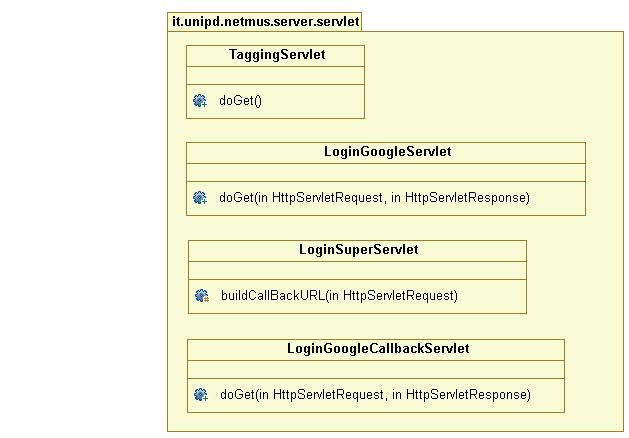
\includegraphics[width=11cm]{img/DP/classes_servlet.png}
\caption{Diagramma UML delle classi che descrive le dipendenze
fondamentali presenti all'interno del package
\emph{it.unipd.netmus.server.servlet}.}
\end{figure}

\subsection*{Requisiti obbligatori soddisfatti}
\begin{itemize}
	\item Nessuno
\end{itemize}
\subsection*{Requisiti desiderabili e opzionali soddisfatti}
\begin{itemize}
    \item C1FO-1.2.1 Pagina login indipendente
\end{itemize}
\subsection*{Tipo, obiettivo e funzione del componente}
Package del server che contiene le classi utilizzate per interfacciarsi a
servizi esterni, come il login utilizzando l'account Google.
\subsection*{Attivit\`a svolte e dati trattati}
Gestisce lo scambio di dati con servizi esterni.


\newpage
\subsection{Classe LoginSuperServlet}
\subsubsection*{Requisiti obbligatori soddisfatti}
\begin{itemize}
    \item Nessuno
\end{itemize}
\subsubsection*{Requisiti desiderabili e opzionali soddisfatti}
\begin{itemize}
    \item C1FO-1.2.1 Pagina login indipendente
\end{itemize}
\subsubsection*{Tipo, obiettivo e funzione del componente}
\`E una classe astratta che estende \co{HttpServlet} ed ha lo scopo di
implementare il metodo di creazione dell'indirizzo di ritorno del richiedente.
\subsubsection*{Attivit\`a svolte e dati trattati}
Crea semplicemente l'URL di Callback per far tornare una risposta HTTP al
client in seguito ad una sua richiesta di login.

\begin{longtable}{|p{0.4\textwidth}|p{0.4\textwidth}|}
\hline
\rowcolor{orange} \bo{Metodo} & \bo{Descrizione} \\
\hline
\endhead
\hline
\multicolumn{2}{|c|}{\textit{continua alla pagina successiva}}\\
\hline
\endfoot
\endlastfoot
 \# buildCallBackURL(in HttpServletRequest) & Crea l'indirizzo di ritorno del
 richiedente, per la richiesta di login. \\\hline
\caption{Metodi di LoginSuperServlet}
\end{longtable}

\newpage
\subsection{Classe LoginGoogleServlet}
\subsubsection*{Requisiti obbligatori soddisfatti}
\begin{itemize}
    \item Nessuno
\end{itemize}
\subsubsection*{Requisiti desiderabili e opzionali soddisfatti}
\begin{itemize}
    \item C1FO-1.2.1 Pagina login indipendente
\end{itemize}
\subsubsection*{Tipo, obiettivo e funzione del componente}
Utilizzata per il login tramite l'account Google.
\subsubsection*{Attivit\`a svolte e dati trattati}
Predispone il servizio e reindirizza l'utente al servizio di login di Google.
Google, dopo che l'utente avr\`a effettuato l'accesso, lo reindizzer\`a nuovamente
al nostro programma trasmettendo a \co{LoginGoogleCallbackServlet} tutte le
informazioni del caso.

\begin{longtable}{|p{0.4\textwidth}|p{0.4\textwidth}|}
\hline
\rowcolor{orange} \bo{Metodo} & \bo{Descrizione} \\
\hline
\endhead
\hline
\multicolumn{2}{|c|}{\textit{continua alla pagina successiva}}\\
\hline
\endfoot
\endlastfoot
+ doGet(in HttpServletRequest, in HttpServletResponse) & Crea ed invia una
richiesta al servizio di login Google per fargli mostrare la pagina di login
predefinita per i Google Account. \\\hline
\caption{Metodi di LoginGoogleServlet}
\end{longtable}

\newpage
\subsection{Classe LoginGoogleCallbackServlet}
\subsubsection*{Requisiti obbligatori soddisfatti}
\begin{itemize}
    \item Nessuno
\end{itemize}
\subsubsection*{Requisiti desiderabili e opzionali soddisfatti}
\begin{itemize}
    \item C1FO-1.2.1 Pagina login indipendente
\end{itemize}
\subsubsection*{Tipo, obiettivo e funzione del componente}
Utilizzata per il login tramite l'account Google.
\subsubsection*{Attivit\`a svolte e dati trattati}
Riceve i dati dell'account dell'utente dopo che quest'ultimo ha effettuato
l'accesso tramite il Google account. Se \`e la prima volta che l'utente entra in
NetMus viene creato in automatico un account personale con lo stesso ID del
Google Account. Se esiste gi\`a viene semplicemente autenticata la sessione
corrente. Se esiste gi\`a un utente NetMus con lo stesso ID non potr\`a essere
registrato tale utente Google, e quindi sar\`a reindirizzato alla pagina di
Login.

\begin{longtable}{|p{0.4\textwidth}|p{0.4\textwidth}|}
\hline
\rowcolor{orange} \bo{Metodo} & \bo{Descrizione} \\
\hline
\endhead
\hline
\multicolumn{2}{|c|}{\textit{continua alla pagina successiva}}\\
\hline
\endfoot
\endlastfoot
+ doGet(in HttpServletRequest, in HttpServletResponse) & Gestisce l'arrivo di
una risposta da Google, che porta l'utente loggato con Google Account. Se
questo \`e null, allora non \`e andata a buon fine l'autenticazione Google. Se
invece \`e andata a buon fine viene associata all'utente la sessione corrente.
\\\hline
\caption{Metodi di LoginGoogleCallbackServlet}
\end{longtable}


\newpage
\section{Package server.utils} % LASCIARE WARNING

\begin{figure}[!h]
  \centering
  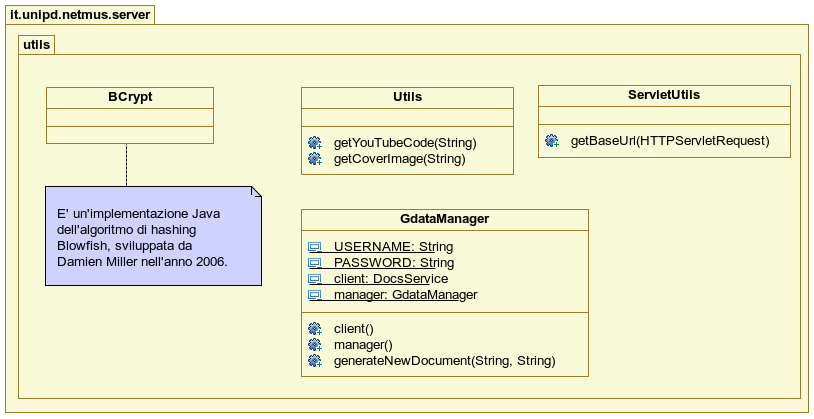
\includegraphics[width=14cm]{img/DP/classes_server_utils.png}
\caption{Diagramma UML delle classi che descrive le dipendenze
fondamentali presenti all'interno del package
\emph{it.unipd.netmus.server.utils}.}
\end{figure}

\subsection*{Requisiti obbligatori soddisfatti}
\begin{itemize}
    \item C1QN-2.6 Manutenibilit\`a
\end{itemize}
\subsection*{Requisiti desiderabili e opzionali soddisfatti}
\begin{itemize}
    \item Nessuno
\end{itemize}
\subsection*{Tipo, obiettivo e funzione del componente}
Contiene le classi che forniscono funzioni di utilit\`a comunemente utilizzate
dalle altre classi del package \emph{server}.
\subsection*{Attivit\`a svolte e dati trattati}
Varie.

\subsection{Classe BCrypt}
\subsubsection*{Requisiti obbligatori soddisfatti}
\begin{itemize}
    \item C1FN-1.2 Registrazione a NetMus
    \item C1FN-1.4.2 Cambio password
\end{itemize}
\subsection*{Requisiti desiderabili e opzionali soddisfatti}
\begin{itemize}
    \item Nessuno
\end{itemize}
\subsubsection*{Tipo, obiettivo e funzione del componente}
Questa classe \`e stata importata nel progetto con lo scopo di fornirci uno
strumento semplice ma efficace per cifrare le password dei nostri utenti, prima
di essere memorizzate nel DataStore. \`E un'implementazione Java dell'algoritmo
di hashing Blowfish, sviluppata da Damien Miller nell'anno 2006.
 \subsubsection*{Attivit\`a svolte e dati trattati}
Svolge l'attivit\`a di cifratura delle password del sistema NetMus.
\\\\
Non verranno elencati nel dettaglio i metodi ed i campi dati poich\'e questa
classe \`e importata nel progetto e ci offre un servizio black-box.

\subsection{Classe Utils}
\subsubsection*{Requisiti obbligatori soddisfatti}
\begin{itemize}
    \item C1FN-1.9 Ricezione ed elaborazione dei brani
\end{itemize}
\subsection*{Requisiti desiderabili e opzionali soddisfatti}
\begin{itemize}
    \item C1QD-1.5.1 Ottimizzazione della ricerca su YouTube
    \item C1VD-1.5.2 Quote YouTube
    \item C1VD-1.5.3 YouTube Terms of Services
    \item C1FO-1.9.3 Completamento info da servizio esterno
\end{itemize}
\subsubsection*{Tipo, obiettivo e funzione del componente}
Questa classe deve offrire dei metodi statici semplici per avere accesso ai
servizi esterni YouTube e Last.fm. Si occuper\`a di prelevare il codice
del video riproducibile su YouTube, mettendo in ingresso come keyword l'artista
ed il titolo del brano. Dovr\`a in ugual modo andare ad interrogare il database
di Last.fm per poter prelevare la copertina relativa al brano, oppure
informazioni riguardanti artista e album se mancanti nel tag del brano e nel
nostro database interno.
\subsubsection*{Attivit\`a svolte e dati trattati}
Classe di servizio per interrogare servizi esterni, con lo scopo di completare
le informazioni su un brano il pi\`u possibile, in maniera da offrire il
maggior numero di funzionalit\`a per quel brano.

\begin{longtable}{|p{0.4\textwidth}|p{0.4\textwidth}|}
\hline
\rowcolor{orange} \bo{Metodo} & \bo{Descrizione} \\
\hline
\endhead
\hline
\multicolumn{2}{|c|}{\textit{continua alla pagina successiva}}\\
\hline
\endfoot
\endlastfoot
 + getYouTubeCode(in String, in String) static & Grazie a YouTubeManager
 restituisce la prima occorrenza di una ricerca su YouTube per pertinenza alla keyword in ingresso
 (autore titolo). Se la ricerca non produce risultati restituisce stringa vuota.
 Viene utilizzato nella ricerca anche l'indirizzo IP del client, per poter
 raffinare la ricerca, in maniera che i contenuti dei video trovati siano
 realmente riproducibili. \\\hline 
 - getYouTubeCode(in String, in String, in
 int) static & Metodo privato utilizzato per fornire il comportamento atteso da \emph{getYouTubeCode} in
  maniera ricorsiva per ritentare la ricerca quante volte specificato, in caso
  di fallimento. \\\hline
  + getCoverImage(in String) static & Questo metodo attiva la cache di Last.fm
  per AppEngine ed esegue una ricerca esterna, con keyword artista e album,
  per recuperare l'url della copertina dell'album relativo ad un brano, in
  formato JPG. \\\hline
  + getSongFromFileName(in String) static & Con questo metodo andremo
  a provare a recuperare informazioni ulteriori di un brano che non ha info nel tag,
  usando come keyword il nome del file stesso. Se verr\`a trovato qualcosa si
  prover\`a a proporlo all'utente. In uscita restituir\`a un SongDTO. \\\hline
\caption{Metodi di Utils}
\end{longtable}

\subsection{Classe ServletUtils}
\subsubsection*{Requisiti obbligatori soddisfatti}
\begin{itemize}
    \item Nessuno
\end{itemize}
\subsubsection*{Requisiti desiderabili e opzionali soddisfatti}
\begin{itemize}
    \item C1FO-1.2.1 Pagina login indipendente
\end{itemize}
\subsubsection*{Tipo, obiettivo e funzione del componente}
Questa classe conterr\`a metodi utili alle servlet per la gestione degli
indirizzi della applicazione.
\subsubsection*{Attivit\`a svolte e dati trattati}
Funzioni utili alle servlet per la gestione degli URL.

\begin{longtable}{|p{0.4\textwidth}|p{0.4\textwidth}|}
\hline
\rowcolor{orange} \bo{Metodo} & \bo{Descrizione} \\
\hline

 + getBaseUrl(in HttpServletRequest) static & Questo metodo deve tornare
 l'indirizzo di base dell'applicazione, a seconda di dove \`e hostato il
 progetto e da che porta viene acceduto. \\\hline
\caption{Metodi di ServletUtils}
\end{longtable}

\subsection{Classe GdataManager}
\subsubsection*{Requisiti obbligatori soddisfatti}
\begin{itemize}
  \item Nessuno
\end{itemize}
\subsubsection*{Requisiti desiderabili e opzionali soddisfatti}
\begin{itemize}
  \item C1FO-1.8.1 Esportazione PDF
\end{itemize}
\subsubsection*{Tipo, obiettivo e funzione del componente}
  La classe \`e un singleton che ha lo scopo di fornire i metodi per la gestione 
  (creazione, modifica, inserimento e rimozione) di documenti e di
  account Google Docs.
  
   \subsubsection*{Attivit\`a svolte e dati
trattati}
\begin{longtable}{|p{0.4\textwidth}|p{0.4\textwidth}|}
\hline
\rowcolor{orange} \bo{Attributo} & \bo{Descrizione} \\
\hline
\endhead
\hline
\multicolumn{2}{|c|}{\textit{continua alla pagina successiva}}\\
\hline
\endfoot
\endlastfoot
- USERNAME: String \emph{static} & Email dell'account di Google Docs in
uso.\\\hline
 - PASSWORD: String \emph{static} & Password dell'account di Google
Docs in uso.\\\hline
 - manager: GdataManager \emph{static} & Unica istanza della
classe \co{GdataManager}.\\\hline
 - client: DocsService \emph{static} & Istanza dell'account di
 autenticazione in Google Docs.\\\hline
\caption{Campi dati di GdataManager}
\end{longtable}
\begin{longtable}{|p{0.4\textwidth}|p{0.4\textwidth}|}
\hline
\rowcolor{orange} \bo{Metodo} & \bo{Descrizione} \\
\hline
\endhead
\hline
\multicolumn{2}{|c|}{\textit{continua alla pagina successiva}}\\
\hline
\endfoot
\endlastfoot
+ manager(): GdataManager \emph{static} & Crea l'istanza di
\co{GdataManager}\\\hline
+ client(): DocsService & Inizializza \co{client} e verifica i
dati di accesso.\\\hline 
+ getDocument(String): DocumentListEntry & Restituisce il documento
associato al parametro \co{id}.\\\hline
+ getFolder(): DocumentListEntry & Restituisce la cartella nella quale
verr\`a creato il file, cos\'\i\ da applicarli permessi
pubblici. Solo gli utenti reindirizzati a tale
documento avranno accesso al documento.\\\hline
+ createNewDocument(String,String) :
DocumentListEntry & Crea un nuovo documento in base hai parametri titolo e contenuto.\\\hline
\caption{Metodi di GdataManager}
\end{longtable}

\newpage
\subsection{Dettaglio su creazione Google Docs del catalogo}

\begin{figure}[!h]
  \centering
  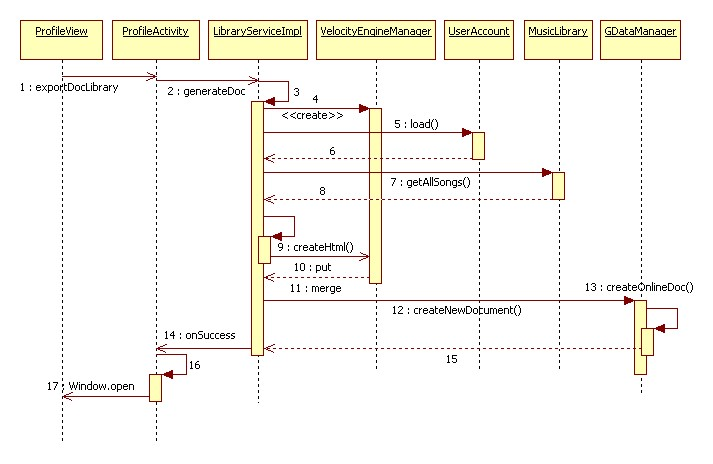
\includegraphics[width=17cm]{img/DP/export_gdocs.png}
\caption{Diagramma UML di sequenza che descrive la procedura di creazione del
documento condiviso su Google Docs e sua visualizzazione.}
\end{figure}

Quando un utente clicca su \bo{Genera Doc} parte la richiesta a
\co{ProfileActivity} che a sua volta manda una RPC a \co{LibraryService}, che fa
partire su server la creazione del documento.\\\\
Viene inizializzato il VelocityEngineManager che si occuper\`a della creazione
del testo formatto in maniera opportuna, utile alla creazione del Docs.\\\\
Viene estratta la libreria dell'utente che la richiede, generata una lista
ordinata contenente tutti i brani della libreria e viene mandata in elaborazione
come VelocityContext. Il testo generato poi sar\`a necessario per creare il vero
e proprio documento online.\\\\
Una volta generato questo testo viene appunto importato dentro un file di Google
Docs, che verr\`a creato in una cartella pubblica in maniera da far accedere a
tale documento solamente chi ne possiede il link, anche senza
autenticazione.\\\\
L'indirizzo a tale documento poi verr\`a utilizzato, al ritorno della RPC, per
mostrarlo su una nuova finestra del browser del client.\\
Alcuni browser possono limitare tale apertura per eventuali blocchi popup
impostati, baster\`a in quel caso dare il permesso a tali popup.


\newpage
\section{Package server.utils.cache} % LASCIARE WARNING
\subsection*{Requisiti obbligatori soddisfatti}
\begin{itemize}
    \item C1QN-1.6 Scalabilit\`a
    \item C1QN-1.6.2 Scalabilit\`a massa di utenza
\end{itemize}
\subsection*{Requisiti desiderabili e opzionali soddisfatti}
\begin{itemize}
    \item Nessuno
\end{itemize}
\subsection*{Tipo, obiettivo e funzione del componente}
Il package \emph{cache} racchiude al suo interno le classi necessarie alla
gestione della Memcache e che utilizzano il framework JCache. Come per il resto
delle componenti presenti in \emph{utils} fornisce all'esterno alcune utilit\`a
disponibili a tutto il lato server. 
\subsection*{Attivit\`a svolte e dati trattati} L'unica classe contenuta,
\co{CacheSupport}, fornisce un insieme di metodi pubblici necessari per
utilizzare la cache. Contiene inoltre un'interfaccia utilizzata per marcare le
entit\`a ``persistenti'' della Memcache.


\subsection{Interfaccia Cacheable}
\subsubsection*{Requisiti obbligatori soddisfatti}
\begin{itemize}
    \item C1QN-1.6 Scalabilit\`a
    \item C1QN-1.6.2 Scalabilit\`a massa di utenza
\end{itemize}
\subsubsection*{Requisiti desiderabili e opzionali soddisfatti}
\begin{itemize}
    \item Nessuno
\end{itemize}
\subsubsection*{Tipo, obiettivo e funzione del componente} Una semplice
interfaccia che contiene la definizione dei metodi necessari e sufficenti per
rendere una sottoclasse memorizzabile ed estraibile dalla Memcache.
\subsubsection*{Attivit\`a svolte e dati trattati} Viene utilizzata come
marcatore per distinguere quelle classi che sono utilizzate come entit\`a
nella memoria cache.
\begin{longtable}{|p{0.4\textwidth}|p{0.4\textwidth}|}
\hline
\rowcolor{orange} \bo{Metodo} & \bo{Descrizione} \\
\hline
\endhead
\hline
\multicolumn{2}{|c|}{\textit{continua alla pagina successiva}}\\
\hline
\endfoot
\endlastfoot
+ addToCache() & Salva l'oggetto all'interno della Memcache.\\\hline
+ removeFromCache() & Rimuove l'oggetto dalla Memcache.\\\hline
\caption{Metodi di Cacheable}
\end{longtable}

\subsection{Classe CacheSupport}
\subsubsection*{Requisiti obbligatori soddisfatti}
\begin{itemize}
    \item C1QN-1.6 Scalabilit\`a
    \item C1QN-1.6.2 Scalabilit\`a massa di utenza
\end{itemize}
\subsubsection*{Requisiti desiderabili e opzionali soddisfatti}
\begin{itemize}
    \item Nessuno
\end{itemize}
\subsubsection*{Tipo, obiettivo e funzione del componente} \co{CacheSupport} \`e
composta da soli metodi statici che forniscono le principali funzioni
disponibili sulla Memcache. Questi servizi sono disponibili a tutte le
componenti del lato server.
\subsubsection*{Attivit\`a svolte e dati trattati} Rende disponibili all'esterno
le funzioni basilari di lettura e scrittura sulla memoria cache in modo
completamente trasparente rispetto all'implmentazione tramite JCache e
soprattutto all'utilizzo della \co{CacheFactory}.
\begin{longtable}{|p{0.4\textwidth}|p{0.4\textwidth}|}
\hline
\rowcolor{orange} \bo{Metodo} & \bo{Descrizione} \\
\hline
\endhead
\hline
\multicolumn{2}{|c|}{\textit{continua alla pagina successiva}}\\
\hline
\endfoot
\endlastfoot
+ cacheInit(): Cache \emph{static} & Restituisce l'istanza della Memcache
utilizzata. Questo metodo \`e privato poich\'e la configurazione della Memcache
\`e interamente gestita in questa classe.\\\hline
+ cacheGet(in String): Object \emph{static} & Carica dalla mappa della Memcache
l'oggetto la cui chiave \`e data in input.\\\hline 
+ cacheClear() \emph{static} & Ripulisce l'intera Memcache. \\\hline
+ cacheRemove(in String) \emph{static} & Rimuove dalla Memcache l'oggetto
relativo alla chiave data in input.\\\hline
+ cachePut(in String, in Serializable) \emph{static} & Salva nella Memcache
l'oggetto e la relativa chiave dati in input.\\\hline
\caption{Metodi di CacheSupport}
\end{longtable}



\newpage
\section{Package server.utils.velocity} % LASCIARE WARNING
\subsection*{Requisiti obbligatori soddisfatti}
\begin{itemize}
    \item Nessuno
\end{itemize}
\subsection*{Requisiti desiderabili e opzionali soddisfatti}
\begin{itemize}
    \item C1FO-1.8.1 Esportazione PDF
\end{itemize}
\subsection*{Tipo, obiettivo e funzione del componente}
Le classi contenute nel package hanno lo scopo di applicare un template html
alle informazioni sul catalogo utente, dando modo di agire sulla formattazione
della pagina generata tramite Google Docs.
\subsection*{Attivit\`a svolte e dati trattati}
 Attivit\`a e dati saranno approfonditi nella descrizione specifica delle
 classi.

\subsection{Classe VelocityEngineManager}
\subsubsection*{Requisiti obbligatori soddisfatti}
\begin{itemize}
  \item Nessuno
\end{itemize}
\subsubsection*{Requisiti desiderabili e opzionali soddisfatti}
\begin{itemize}
  \item C1FO-1.8.1 Esportazione PDF
\end{itemize}
\subsubsection*{Tipo, obiettivo e funzione del componente}
La classe crea e inizializza l'oggetto``engine'' di tipo \co{VelocityEngine}
\subsubsection*{Attivit\`a svolte e dati trattati}
Vengono settate le propriet\`a dell'engine che poi viene avviato.
\begin{longtable}{|p{0.45\textwidth}|p{0.45\textwidth}|}
\hline
\rowcolor{orange} \bo{Attributo} & \bo{Descrizione} \\
\hline
\endhead
\hline
\multicolumn{2}{|c|}{\textit{continua alla pagina successiva}}\\
\hline
\endfoot
\endlastfoot
\# engine: VelocityEngine \emph{static} & Velocity template engine.\\\hline
\# init: boolean emph{static} & Traccia lo stato di inizializzazione di
\co{engine}\\\hline
\caption{Campi dati di VelocityEngineManager}
\end{longtable}
\begin{longtable}{|p{0.4\textwidth}|p{0.4\textwidth}|}
\hline
\rowcolor{orange} \bo{Metodo} & \bo{Descrizione} \\
\hline
\endhead
\hline
\multicolumn{2}{|c|}{\textit{continua alla pagina successiva}}\\
\hline
\endfoot
\endlastfoot
+ init() \emph{static} & avvia \co{engine} e ne setta le propriet\`a.\\\hline
\caption{Metodi di VelocityEngineManager}
\end{longtable}


\newpage
\section{Package server.youtube} % LASCIARE WARNING
\subsection*{Requisiti obbligatori soddisfatti}
\begin{itemize}
    \item C1FN-1.9 Ricezione ed elaborazione dei brani
\end{itemize}
\subsection*{Requisiti desiderabili e opzionali soddisfatti}
\begin{itemize}
    \item C1FD-1.1.4 Visualizza player YouTube
    \item C1FD-1.5 Riproduzione tracce in streaming
    \item C1VD-1.5.2 Quote YouTube
    \item C1VD-1.5.3 YouTube Terms of Services
\end{itemize}
\subsection*{Tipo, obiettivo e funzione del componente}
In questo package verranno inserite le classi necessarie all'interazione con le
API di YouTube, tramite le quali andremo ad eseguire le ricerche relative ai
nuovi brani inseriti nel DataStore, per associare ad essi il codice utile alla
riproduzione video.
\subsection*{Attivit\`a svolte e dati trattati}
Ci permettono di fare ricerche video nel database di YouTube.

\subsection{Classe YouTubeMedia}
\subsubsection*{Requisiti obbligatori soddisfatti}
\begin{itemize}
    \item C1FN-1.9 Ricezione ed elaborazione dei brani
\end{itemize}
\subsubsection*{Requisiti desiderabili e opzionali soddisfatti}
\begin{itemize}
    \item C1FD-1.1.4 Visualizza player YouTube
    \item C1FD-1.5 Riproduzione tracce in streaming
    \item C1VD-1.5.2 Quote YouTube
    \item C1VD-1.5.3 YouTube Terms of Services
\end{itemize}
\subsubsection*{Tipo, obiettivo e funzione del componente}
Questa classe ha la funzionalit\`a di contenitore per gestire i principali
dati di un media YouTube, cio\`e il tipo e l'URL.
\subsubsection*{Attivit\`a svolte e dati trattati}
Mantiene l'informazione del URL e del tipo di media.

\begin{longtable}{|p{0.45\textwidth}|p{0.45\textwidth}|}
\hline
\rowcolor{orange} \bo{Attributo} & \bo{Descrizione} \\
\hline
\endhead
\hline
\multicolumn{2}{|c|}{\textit{continua alla pagina successiva}}\\
\hline
\endfoot
\endlastfoot
- type: String & Rappresenta il tipo di dato YouTube relativo ad un
video.\\\hline
- location: String & Rappresenta l'indirizzo di tale dato YouTube.\\\hline
\caption{Campi dati di YouTubeMedia}
\end{longtable}

\begin{longtable}{|p{0.45\textwidth}|p{0.45\textwidth}|}
\hline
\rowcolor{orange} \bo{Metodo} & \bo{Descrizione} \\
\hline
\endhead
\hline
\multicolumn{2}{|c|}{\textit{continua alla pagina successiva}}\\
\hline
\endfoot
\endlastfoot
+ getters() & Restituiscono i campi dati privati della classe.\\\hline
+ setters() & Modificano i campi dati privati della classe.\\\hline
\caption{Metodi di YouTubeMedia}
\end{longtable}

\subsection{Classe YouTubeVideo}
\subsubsection*{Requisiti obbligatori soddisfatti}
\begin{itemize}
    \item C1FN-1.9 Ricezione ed elaborazione dei brani
\end{itemize}
\subsubsection*{Requisiti desiderabili e opzionali soddisfatti}
\begin{itemize}
    \item C1FD-1.1.4 Visualizza player YouTube
    \item C1FD-1.5 Riproduzione tracce in streaming
    \item C1VD-1.5.2 Quote YouTube
    \item C1VD-1.5.3 YouTube Terms of Services
\end{itemize}
\subsubsection*{Tipo, obiettivo e funzione del componente}
Questa classe \`e un ulteriore classe contenitore che si occupa di contenere una
lista di\\ \co{YouTubeMedia} ed il relativo URL.
\subsubsection*{Attivit\`a svolte e dati trattati}
Contiene tutte le informazioni dei media trovati, dopo una ricerca nei database
di YouTube.

\begin{longtable}{|p{0.45\textwidth}|p{0.45\textwidth}|}
\hline
\rowcolor{orange} \bo{Attributo} & \bo{Descrizione} \\
\hline
\endhead
\hline
\multicolumn{2}{|c|}{\textit{continua alla pagina successiva}}\\
\hline
\endfoot
\endlastfoot
- medias: List\textless YouTubeMedia\textgreater & Rappresenta la lista di media
relativi ad una ricerca.\\\hline
- video\_code: String & Rappresenta l'indirizzo di tale ricerca.\\\hline
\caption{Campi dati di YouTubeVideo}
\end{longtable}

\begin{longtable}{|p{0.45\textwidth}|p{0.45\textwidth}|}
\hline
\rowcolor{orange} \bo{Metodo} & \bo{Descrizione} \\
\hline
\endhead
\hline
\multicolumn{2}{|c|}{\textit{continua alla pagina successiva}}\\
\hline
\endfoot
\endlastfoot
+ getters() & Restituiscono i campi dati privati della classe.\\\hline
+ setters() & Modificano i campi dati privati della classe.\\\hline
+ retrieveHttpLocation() : String & Restituisce l'URL di un certo
YouTubeMedia.\\\hline
\caption{Metodi di YouTubeVideo}
\end{longtable}

\subsection{Classe YouTubeManager}
\subsubsection*{Requisiti obbligatori soddisfatti}
\begin{itemize}
    \item C1FN-1.9 Ricezione ed elaborazione dei brani
\end{itemize}
\subsubsection*{Requisiti desiderabili e opzionali soddisfatti}
\begin{itemize}
    \item C1FD-1.1.4 Visualizza player YouTube
    \item C1FD-1.5 Riproduzione tracce in streaming
    \item C1VD-1.5.2 Quote YouTube
    \item C1VD-1.5.3 YouTube Terms of Services
\end{itemize}
\subsubsection*{Tipo, obiettivo e funzione del componente}
Questa classe gestisce effettivamente l'interazione con le API di YouTube per
permetterci di effettuare una ricerca video.
\subsubsection*{Attivit\`a svolte e dati trattati}
Gestisce una richiesta di ricerca video e deve principalmente restituire con
il codice del video pi\`u attinente alle keyword in ingresso nel metodo
\emph{getSearchResult(String keyword)}.

\begin{longtable}{|p{0.45\textwidth}|p{0.45\textwidth}|}
\hline
\rowcolor{orange} \bo{Attributo} & \bo{Descrizione} \\
\hline
\endhead
\hline
\multicolumn{2}{|c|}{\textit{continua alla pagina successiva}}\\
\hline
\endfoot
\endlastfoot
- YOUTUBE\_URL: String \emph{static final} & Rappresenta l'indirizzo
per comunicare con le API \emph{gdata} di YouTube.\\\hline
\caption{Campi dati di YouTubeManager}
\end{longtable}

\begin{longtable}{|p{0.45\textwidth}|p{0.45\textwidth}|}
\hline
\rowcolor{orange} \bo{Metodo} & \bo{Descrizione} \\
\hline
\endhead
\hline
\multicolumn{2}{|c|}{\textit{continua alla pagina successiva}}\\
\hline
\endfoot
\endlastfoot
- retrieveVideo(in String, in String, in int) : YouTubeVideo \emph{static} &
Metodo interno che effettua la ricerca video dati in ingresso un clientID, una
String contenente le keyword ed il tempo di timeout.\\\hline
- convertVideos(in List\textless VideoEntry\textgreater) : YouTubeVideo
\emph{static} & Converte la lista di video trovati nel nostro formato interno
\co{YouTubeVideo} e restituisce solo il risultato in cima alla lista,
che \`e il pi\`u rilevante della ricerca, cio\`e quello che interessa a
noi.\\\hline
+ getSearchResult(in String) : String \emph{static} & Metodo statico usabile
dalle altre classi. Esegue una nuova ricerca e restituisce il codice
del video pi\`u rilevante. Nella query di ricerca utilizzata viene tenuto conto
del IP dell'utente, delle limitazioni all'embedded date dai proprietari dei
video, ai filtri famiglia per evitare contenuti non consoni.\\\hline

\caption{Metodi di YouTubeManager}
\end{longtable}

\newpage
\section{Package shared}

\begin{figure}[!h]
  \centering
  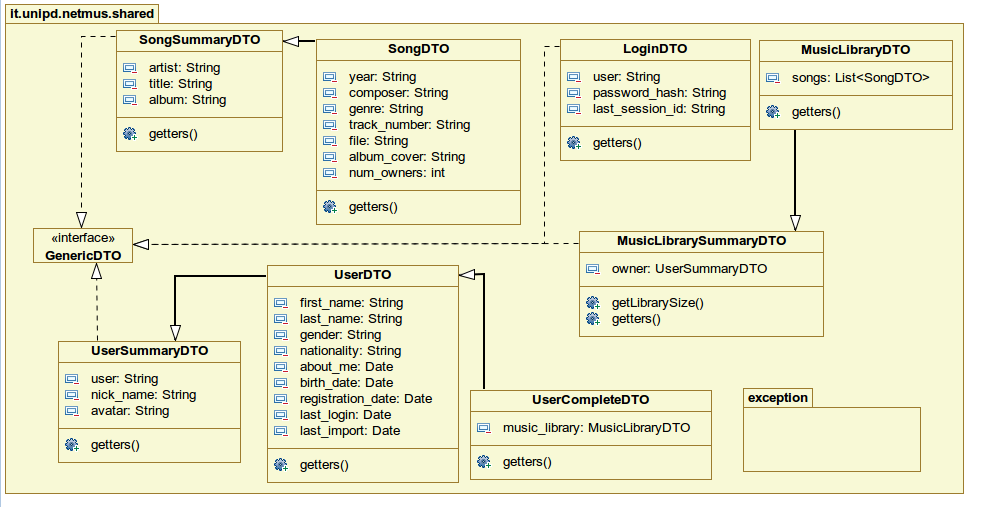
\includegraphics[width=15cm]{img/DP/classes_shared.png}
\caption{Diagramma UML delle classi che descrive le dipendenze
fondamentali presenti all'interno del package
\emph{it.unipd.netmus.shared}.}
\end{figure}

\subsection*{Requisiti obbligatori soddisfatti}
\begin{itemize}
  	\item C1QN-2.6 Manutenibilit\`a
\end{itemize}
\subsection*{Requisiti desiderabili e opzionali soddisfatti}
\begin{itemize}
    \item Nessuno
\end{itemize}
\subsection*{Tipo, obiettivo e funzione del componente}
Il package \emph{shared} contiene le classi degli oggetti che vengono
scambiati tra client e server; in particolare sono presenti le classi che
aderiscono al pattern DTO. L'insieme di queste classi rappresenta tutti i
dati contenuti nelle entit\`a del DataStore opportunamente organizzati in modo
da essere raggruppate in componenti minori e prive di parte logica.
\`E qui contenuta anche la gerarchia delle eccezioni del sistema NetMus.
\subsection*{Attivit\`a svolte e dati trattati}
Le classi di questo package si occupano di inglobare e trasportare
le informazioni attraverso la rete, per le comunicazioni tra server e client,
in particolare i dati relativi alle entit\`a del DataStore ed alle eccezioni.
Vengono qui di seguito descritte pi\`u in dettaglio.

\subsection{Classe UserDTO}
\subsubsection*{Requisiti obbligatori soddisfatti}
\begin{itemize}
	\item C1FN-1.4 Gestione profilo personale
	\item C1FN-1.4.1 Modifica informazioni personali
	\item C1FN-1.4.2 Cambio password
	\item C1FN-1.4.3 Cancellazione del proprio account
\end{itemize}
\subsubsection*{Requisiti desiderabili e opzionali soddisfatti}
\begin{itemize}
    \item C1FD-1.3 Personalizzazione del catalogo
\end{itemize}
\subsubsection*{Tipo, obiettivo e funzione del componente}
Contiene e rappresenta la maggior parte dei dati di un utente, pi\`u
precisamente quelli che ci si aspetta che ogni utente abbia inserito.
\subsubsection*{Attivit\`a svolte e dati trattati}
Funge da contenitore per i dati richiesti di un utente.
\begin{longtable}{|p{0.4\textwidth}|p{0.4\textwidth}|}
\hline
\rowcolor{orange} \bo{Attributo} & \bo{Descrizione} \\
\hline
\endhead
\hline
\multicolumn{2}{|c|}{\textit{continua alla pagina successiva}}\\
\hline
\endfoot
\endlastfoot
 - user\_name: String & indrizzo e-mail valido e univoco dell'utente.\\\hline
 - nick\_name: String & Nickname dell'utente.\\\hline
 - first\_name: String & Nome proprio dell'utente.\\\hline
 - last\_name: String & Cognome dell'utente.\\\hline
 - gender: char & Sesso, sono validi i valori 'F' (femmina) e 'M'
 (maschio).\\\hline
 - nationality: String & Nazione di provenienza dell'utente.\\\hline
 - about\_me: String & Informazioni aggiuntive su
 di se inserite dall'utente.\\\hline
\caption{Campi dati di UserDTO}
\end{longtable}
\begin{longtable}{|p{0.4\textwidth}|p{0.4\textwidth}|}
\hline
\rowcolor{orange} \bo{Metodo} & \bo{Descrizione} \\
\hline
\endhead
\hline
\multicolumn{2}{|c|}{\textit{continua alla pagina successiva}}\\
\hline
\endfoot
\endlastfoot
 + getters() & Tutti gli attributi privati di questa classe hanno i
relativi metodi \emph{get}.\\\hline
 + setters() & Tutti gli attributi privati di questa classe hanno i
relativi metodi \emph{set}.\\\hline
\caption{Metodi di UserDTO}
\end{longtable}


\subsection{Classe UserCompleteDTO}
\subsubsection*{Requisiti obbligatori soddisfatti}
\begin{itemize}
    \item C1FN-1.4 Gestione profilo personale
    \item C1FN-1.4.1 Modifica informazioni personali
    \item C1FN-1.4.2 Cambio password
    \item C1FN-1.4.3 Cancellazione del proprio account
\end{itemize}
\subsubsection*{Requisiti desiderabili e opzionali soddisfatti}
\begin{itemize}
    \item C1FD-1.3 Personalizzazione del catalogo
\end{itemize}
\subsubsection*{Tipo, obiettivo e funzione del componente}
Contiene e rappresenta tutti i dati di un utente, a partire da quelli
visualizzati sul profilo fino a quelli interni del sistema. In particolare
contiene la libreria musicale dell'utente. 
\subsubsection*{Attivit\`a svolte e dati trattati}
Funge da contenitore per tutti dati dell'utente.
\begin{longtable}{|p{0.4\textwidth}|p{0.4\textwidth}|}
\hline
\rowcolor{orange} \bo{Attributo} & \bo{Descrizione} \\
\hline
\endhead
\hline
\multicolumn{2}{|c|}{\textit{continua alla pagina successiva}}\\
\hline
\endfoot
\endlastfoot
 - music\_library: MusicLibraryDTO & Oggetto DTO che rappresenta il
 catalogo multimediale dell'utente.\\\hline
\caption{Campi dati di UserCompleteDTO}
\end{longtable}
\begin{longtable}{|p{0.4\textwidth}|p{0.4\textwidth}|}
\hline
\rowcolor{orange} \bo{Metodo} & \bo{Descrizione} \\
\hline
\endhead
\hline
\multicolumn{2}{|c|}{\textit{continua alla pagina successiva}}\\
\hline
\endfoot
\endlastfoot
 + getters() & Tutti gli attributi privati di questa classe hanno i
relativi metodi \emph{get}.\\\hline
 + setters() & Tutti gli attributi privati di questa classe hanno i
relativi metodi \emph{set}.\\\hline
\caption{Metodi di UserCompleteDTO}
\end{longtable}

\subsection{Classe SongSummaryDTO}
\subsubsection*{Requisiti obbligatori soddisfatti}
\begin{itemize}
    \item Nessuno
\end{itemize}
\subsubsection*{Requisiti desiderabili e opzionali soddisfatti}
\begin{itemize}
    \item C1FD-1.1.4 Visualizza player YouTube
    \item C1FD-1.3 Personalizzazione del catalogo
    \item C1FD-1.3.1 Cancellazione brano
    \item C1FO-1.3.4 Ranking brani
    \item C1FD-1.5 Riproduzione tracce in streaming
\end{itemize}
\subsubsection*{Tipo, obiettivo e funzione del componente}
Contiene e rappresenta i dati pi\`u comunemente utilizzati di un brano, ovvero
quelli che vengono visualizzati in una playlist all'interno di un profilo.
\subsubsection*{Attivit\`a svolte e dati trattati}
Funge da contenitore per i dati pi\`u comunemente utilizzati di un brano, come
per esempio titolo ed autore.
\begin{longtable}{|p{0.4\textwidth}|p{0.4\textwidth}|}
\hline
\rowcolor{orange} \bo{Metodo} & \bo{Descrizione} \\
\hline
\endhead
\hline
\multicolumn{2}{|c|}{\textit{continua alla pagina successiva}}\\
\hline
\endfoot
\endlastfoot
 - title: String & Titolo del brano.\\\hline 
 - artist: String & Nome della band o del cantante autore. \\\hline
 - album: String & Nome dell'album. \\\hline
 - rating: double & Rating generale della canzone rappresentato dalla media di
 tutti i voti assegnati dagli utenti che la condividono \\\hline
 - rating\_for\_this\_user: int & voto assegnato a questa canzone
 dall'utente che possiede la libreria da cui \`e stato estratto questo
 DTO.\\\hline
\caption{Campi dati di SongDTO}
\end{longtable}
\begin{longtable}{|p{0.4\textwidth}|p{0.4\textwidth}|}
\hline
\rowcolor{orange} \bo{Metodo} & \bo{Descrizione} \\
\hline
\endhead
\hline
\multicolumn{2}{|c|}{\textit{continua alla pagina successiva}}\\
\hline
\endfoot
\endlastfoot
 + getters() & Tutti gli attributi privati di questa classe hanno i
relativi metodi \emph{get}.\\\hline
 + setters() & Tutti gli attributi privati di questa classe hanno i
relativi metodi \emph{set}.\\\hline
\caption{Metodi di SongDTO}
\end{longtable}

\subsection{Classe SongDTO}
\subsubsection*{Requisiti obbligatori soddisfatti}
\begin{itemize}
    \item Nessuno
\end{itemize}
\subsubsection*{Requisiti desiderabili e opzionali soddisfatti}
\begin{itemize}
    \item C1FD-1.1.4 Visualizza player YouTube
    \item C1FD-1.3 Personalizzazione del catalogo
    \item C1FD-1.3.1 Cancellazione brano
    \item C1FO-1.3.4 Ranking brani
    \item C1FD-1.5 Riproduzione tracce in streaming
\end{itemize}
\subsubsection*{Tipo, obiettivo e funzione del componente}
Contiene e rappresenta tutti i dati di un brano, compresi quelli interni del
sistema.
\subsubsection*{Attivit\`a svolte e dati trattati}
Funge da contenitore per tutti dati del brano, dal titolo al numero
identificativo del brano. 
\begin{longtable}{|p{0.4\textwidth}|p{0.4\textwidth}|}
\hline
\rowcolor{orange} \bo{Metodo} & \bo{Descrizione} \\
\hline
\endhead
\hline
\multicolumn{2}{|c|}{\textit{continua alla pagina successiva}}\\
\hline
\endfoot
\endlastfoot
- year: String & Anno di pubblicazione del brano.\\\hline
- composer: String & Nome del compositore della canzone.\\\hline
- track\_number: String & Numero della canzone all'interno dell'album.\\\hline
- genre: String & Genere musicale associato alla
 canzone.\\\hline
- file: String & Nome del file da cui sono state estratte le
 informazioni del brano.\\\hline
- album\_cover: String & Link all' immagine della copertina dell'album a cui appartiene il
 brano.\\\hline
- num\_owners: String & Numero di utenti che possiedono la
 canzone nel proprio catalogo.\\\hline
- youtube\_code: String & Codice del rispettivo video su Youtube.\\\hline
- num\_ratings: String & Numero di voti effettuati su questa canzone.\\\hline
\caption{Campi dati di SongDTO}
\end{longtable}
\begin{longtable}{|p{0.4\textwidth}|p{0.4\textwidth}|}
\hline
\rowcolor{orange} \bo{Metodo} & \bo{Descrizione} \\
\hline
\endhead
\hline
\multicolumn{2}{|c|}{\textit{continua alla pagina successiva}}\\
\hline
\endfoot
\endlastfoot
 + getters() & Tutti gli attributi privati di questa classe hanno i
relativi metodi \emph{get}.\\\hline
 + setters() & Tutti gli attributi privati di questa classe hanno i
relativi metodi \emph{set}.\\\hline
\caption{Metodi di SongDTO}
\end{longtable}


\subsection{Classe LoginDTO}
\subsubsection*{Requisiti obbligatori soddisfatti}
\begin{itemize}
	\item C1FN-1.2 Registrazione
\end{itemize}
\subsubsection*{Requisiti desiderabili e opzionali soddisfatti}
\begin{itemize}
    \item Nessuno
\end{itemize}
\subsubsection*{Tipo, obiettivo e funzione del componente}
Contiene e rappresenta i dati di login di un utente.
\subsubsection*{Attivit\`a svolte e dati trattati}
Trasporta nome utente e password dal client al server per
tutte le procedure legate all'autenticazione.
\begin{longtable}{|p{0.4\textwidth}|p{0.4\textwidth}|}
\hline
\rowcolor{orange} \bo{Attributo} & \bo{Descrizione} \\
\hline
\endhead
\hline
\multicolumn{2}{|c|}{\textit{continua alla pagina successiva}}\\
\hline
\endfoot
\endlastfoot
 - user: String & Rappresenta il nome di login unico
dell'utente e nello stesso tempo la sua e-mail (valida).\\\hline
 - password: String & Contiene l'hash della password dell'utente ottenuto
utilizzando l'algoritmo BCrypt.\\\hline
\caption{Campi dati di LoginDTO}
\end{longtable}
\begin{longtable}{|p{0.4\textwidth}|p{0.4\textwidth}|}
\hline
\rowcolor{orange} \bo{Metodo} & \bo{Descrizione} \\
\hline
\endhead
\hline
\multicolumn{2}{|c|}{\textit{continua alla pagina successiva}}\\
\hline
\endfoot
\endlastfoot
 + getters() & Tutti gli attributi privati di questa classe hanno i
relativi metodi \emph{get}.\\\hline
 + setters() & Tutti gli attributi privati di questa classe hanno i
relativi metodi \emph{set}.\\\hline
\caption{Metodi di LoginDTO}
\end{longtable}

\subsection{Classe MusicLibraryDTO}
\subsubsection*{Requisiti obbligatori soddisfatti}
\begin{itemize}
	\item Nessuno
\end{itemize}
\subsubsection*{Requisiti desiderabili e opzionali soddisfatti}
\begin{itemize}
    \item C1FD-1.3 Personalizzazione del catalogo
    \item C1FO-1.3.3 Creazione playlist
    \item C1FO-1.3.4 Ranking brani
\end{itemize}
\subsubsection*{Tipo, obiettivo e funzione del componente}
Contiene le informazioni relative ad un catalogo multimediali compresa la lista
di canzoni di cui \`e composto. Le canzoni presenti nella lista sono incapsulate
in oggetti di tipo \co{SongSummaryDTO} e contengono solamente le informazioni
basilari quali artista e titolo.
\subsubsection*{Attivit\`a svolte e dati trattati}
Fa da contenitore per tutti dati di un catalogo multimediale fornendo solo le
informazioni essenziali per le canzoni.
\begin{longtable}{|p{0.4\textwidth}|p{0.4\textwidth}|}
\hline
\rowcolor{orange} \bo{Attributo} & \bo{Descrizione} \\
\hline
\endhead
\hline
\multicolumn{2}{|c|}{\textit{continua alla pagina successiva}}\\
\hline
\endfoot
\endlastfoot
 - owner: UserSummaryDTO & Dati essenziali relativi all'utente
 associato a questo catalogo.\\\hline 
 - songs: List\textless SongSummaryDTO\textgreater & Lista delle
 canzoni (dati essenziali) presenti nel catalogo.\\\hline
\caption{Campi dati di MusicLibrarySummaryDTO}
\end{longtable}
\begin{longtable}{|p{0.4\textwidth}|p{0.4\textwidth}|}
\hline
\rowcolor{orange} \bo{Metodo} & \bo{Descrizione} \\
\hline
\endhead
\hline
\multicolumn{2}{|c|}{\textit{continua alla pagina successiva}}\\
\hline
\endfoot
\endlastfoot
 + getters() & Tutti gli attributi privati di questa classe hanno i
relativi metodi \emph{get}.\\\hline
 + setters() & Tutti gli attributi privati di questa classe hanno i
relativi metodi \emph{set}.\\\hline
\caption{Metodi di MusicLibrarySummaryDTO}
\end{longtable}

\subsection{Classe FieldVerifier}
\subsubsection*{Requisiti obbligatori soddisfatti}
\begin{itemize}
    \item C1FN-1.2 Registrazione a NetMus
\end{itemize}
\subsubsection*{Requisiti desiderabili e opzionali soddisfatti}
\begin{itemize}
    \item Nessuno
\end{itemize}
\subsubsection*{Tipo, obiettivo e funzione del componente}
Questa semplice classe contiene i metodi statici necessari a validare con
livello di sicurezza accettabile i dati inseriti dall'utente, si rende
fondamentale nelle operazioni di autenticazione e registrazione.
\subsubsection*{Attivit\`a svolte e dati trattati} Le stringhe che vengono
trattate in questa classe sono rappresentate da password, username e indirizzi
email. Per le prime due tipologie di informazione il controllo eseguito si
limita alla lunghezza della stringa, per quanto riguarda gli indirizzi email,
invece, viene verificata l'aderenza agli standard.
\begin{longtable}{|p{0.4\textwidth}|p{0.4\textwidth}|}
\hline
\rowcolor{orange} \bo{Metodo} & \bo{Descrizione} \\
\hline
\endhead
\hline
\multicolumn{2}{|c|}{\textit{continua alla pagina successiva}}\\
\hline
\endfoot
\endlastfoot
 + isValidNickname(in String): boolean \emph{static} & Verifica che la stringa
 in input sia lunga almeno 4 caratteri.\\\hline 
 + isValidPassword(in String): boolean \emph{static} & Verifica che la
 password (non ancora criptata) in input sia lunga almeno 4 caratteri.\\\hline
 + isValidEmail(in String): boolean \emph{static} & Verifica che l'email in
 input sia conforme agli standard.\\\hline
\caption{Metodi di MusicLibraryDTO}
\end{longtable}


\newpage
\section{Package shared.exception}

\begin{figure}[!h]
  \centering
  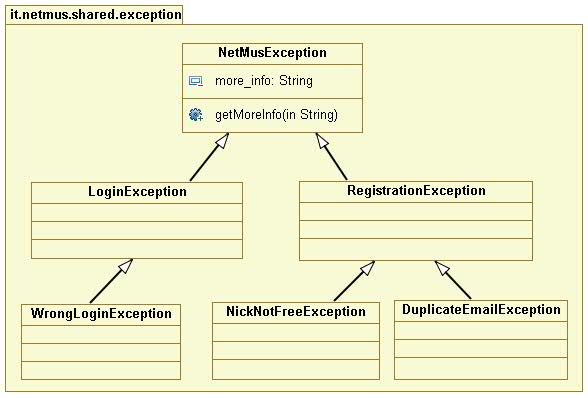
\includegraphics[width=9cm]{img/DP/classes_shared_exception.png}
\caption{Diagramma UML delle classi che descrive le dipendenze
fondamentali presenti all'interno del package
\emph{it.unipd.netmus.shared.exception}.}
\end{figure}


\subsection*{Requisiti obbligatori soddisfatti}
\begin{itemize}
	\item C1QN-2.7 Gestione errori
\end{itemize}
\subsection*{Requisiti desiderabili e opzionali soddisfatti}
\begin{itemize}
    \item Nessuno
\end{itemize}
\subsection*{Tipo, obiettivo e funzione del componente}
Il package \emph{shared.exception} raccoglie le classi che trattano
le eccezioni che posso essere lanciate dal sistema NetMus. Le classi eccezione
sono opportunamente gerarchizzate.
\subsection*{Attivit\`a svolte e dati trattati}
Fornisce tutte le possibili eccezioni che possono essere lanciate dal sistema
NetMus.

\subsection{Classe NetMusException}
\subsubsection*{Requisiti obbligatori soddisfatti}
\begin{itemize}
	\item C1QN-2.7 Gestione errori
\end{itemize}
\subsubsection*{Requisiti desiderabili e opzionali soddisfatti}
\begin{itemize}
    \item Nessuno
\end{itemize}
\subsubsection*{Tipo, obiettivo e funzione del componente}
Generica eccezione del nostro programma.
\subsubsection*{Attivit\`a svolte e dati trattati}
Rappresenta una generica eccezione usata all'interno del sistema NetMus. Tutte
le altre eccezioni estendono questa.

\subsection{Classe LoginException}
\subsubsection*{Requisiti obbligatori soddisfatti}
\begin{itemize}
	\item C1QN-2.7 Gestione errori
\end{itemize}
\subsubsection*{Requisiti desiderabili e opzionali soddisfatti}
\begin{itemize}
    \item Nessuno
\end{itemize}
\subsubsection*{Tipo, obiettivo e funzione del componente}
Indica un generico errore rilevato durante il tentativo di login.
\subsubsection*{Attivit\`a svolte e dati trattati}
Nessuna.

\subsection{Classe RegistrationException}
\subsubsection*{Requisiti obbligatori soddisfatti}
\begin{itemize}
	\item C1QN-2.7 Gestione errori
\end{itemize}
\subsubsection*{Requisiti desiderabili e opzionali soddisfatti}
\begin{itemize}
    \item Nessuno
\end{itemize}
\subsubsection*{Tipo, obiettivo e funzione del componente}
Indica un generico errore rilevato durante la registrazione di un nuovo utente.
\subsubsection*{Attivit\`a svolte e dati trattati}
Nessuna.


\newpage
\section{Applet di estrazione brani}

\begin{figure}[!h]
  \centering
  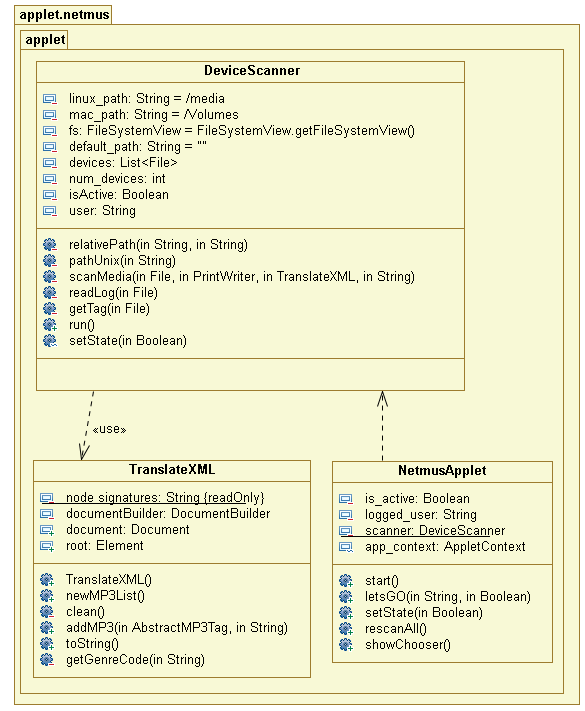
\includegraphics[width=9cm]{img/DP/applet.png}
\caption{Diagramma UML delle classi che descrive le dipendenze
fondamentali presenti all'interno del applet di estrazione dati.}
\end{figure}

\subsection*{Requisiti obbligatori soddisfatti}
\begin{itemize}
	\item C2QN-4.4 Manutenibilit\`a
	\item C2VN-4.6 Norme legali
\end{itemize}
\subsection*{Requisiti desiderabili e opzionali soddisfatti}
\begin{itemize}
    \item Nessuno
\end{itemize}
\subsection*{Tipo, obiettivo e funzione del componente}
L'applet di estrazione brani verr\`a sviluppata come componente
Java indipendente. In seguito sar\`a compilata ed esportata in un file JAR, il
quale verr\`a inserito nel sistema NetMus per essere caricato dinamicamente
dalla classe \co{AppletBar.java} come elemento HTML di tipo \emph{applet}.\\
Una volta caricata nella Profile View di un utente loggato, richieder\`a
l'accettazione di una firma digitale, per avere l'accesso in lettura/scrittura
sul File System del client. In tal modo potr\`a cominciare a monitorare le
periferiche di archiviazione di massa che verranno collegate da quel momento in
poi.
\subsection*{Attivit\`a svolte e dati trattati}
L'applet deve monitorare le periferiche presenti nella macchina client e,
all'inserimento di un nuovo device visibile come periferica di archiviazione di
massa, andr\`a a scansionarlo interamente estraendo tutti i Tag informativi dei
brani Mp3 presenti. Verr\`a creato un file di log interno al device con lo scopo
di tenere traccia, in una scansione futura, dei file che son gi\`a stati
analizzati. Tutti i Tag analizzati verranno tradotti in un elemento XML, infine
spedito alla classe \co{AppletBar.java} sotto forma di stringa.\\

\subsection{Classe NetmusApplet}
\subsubsection*{Requisiti obbligatori soddisfatti}
\begin{itemize}
   \item C2FN-1 Recupero delle informazioni
   \item C2FN-1.1 Recupero automatico
   \item C2FN-1.2 Recupero manuale
   \item C2FN-3 Comunicazione con C1
   \item C2FN-3.1 Invio delle informazioni
   \item C2QN-3.2 Utilizzo della connessione
   \item C2QN-4 Utilizzo
\end{itemize}
\subsubsection*{Requisiti desiderabili e opzionali soddisfatti}
\begin{itemize}
   \item C2FD-1.4 Informazioni dall'hard disk
\end{itemize}
\subsubsection*{Tipo, obiettivo e funzione del componente}
Questa classe sar\`a di tipo \co{JApplet} e si occuper\`a di avviare l'applet
quando caricata in una pagina Web. Quando viene creata invier\`a una notifica a
GWT, il quale andr\`a ad avviare effettivamente il thread di
scansionamento nell'applet, passandogli il nome utente e lo stato di attivazione scelto in precedenza
dall'utente. Di default sar\`a attiva ma pu\`o essere disattivata manualmente.
Quando sar\`a disattivata il thread \co{scanner} viene messo a dormire e verr\`a
svegliato in seguito ad una richiesta dell'utente, tramite il metodo
\co{setState} che andr\`a ad invocare un \co{notify()} sull'oggetto di lock su
cui \co{scanner} si \`e addormentato.
\subsubsection*{Attivit\`a svolte e dati trattati}
Svolge la funzione di avviare l'applet associandola all'utente e con lo
stato da lui impostato. Non ha un'interfaccia grafica sua, ma verr\`a disegnata
in \co{AppletBar} da GWT all'interno di una ``barra di estrazione''.\\
\\

\begin{longtable}{|p{0.4\textwidth}|p{0.4\textwidth}|}
\hline
\rowcolor{orange} \bo{Attributo} & \bo{Descrizione} \\
\hline
\endhead
\hline
\multicolumn{2}{|c|}{\textit{continua alla pagina successiva}}\\
\hline
\endfoot
\endlastfoot
- is\_active: bool & Stato del thread scanner.\\\hline
- logged\_user: String & Nome dell'utente loggato attuale.\\\hline
- scanner: DeviceScanner & Thread di scansione devices.\\\hline
\# app\_context: AppletContext & Context nel quale \`e inserita
l'applet.\\\hline
\caption{Campi dati di NetmusApplet}
\end{longtable}

\begin{longtable}{|p{0.4\textwidth}|p{0.4\textwidth}|}
\hline
\rowcolor{orange} \bo{Metodo} & \bo{Descrizione} \\
\hline
\endhead
\hline
\multicolumn{2}{|c|}{\textit{continua alla pagina successiva}}\\
\hline
\endfoot
\endlastfoot
+ start() & Metodo ereditato da \co{JApplet} invocato in automatico quando
viene caricata la classe nel browser.\\\hline
+ letsGO(in String, in boolean) & Metodo invocato da GWT tramite
JSNI che va a settare il nome utente e fa partire il monitoraggio
del File System da parte di \co{scanner}.\\\hline
+ setState(in boolean) & Metodo per cambiare lo stato del
monitoraggio dello \co{scanner}.\\\hline
\caption{Metodi di NetmusApplet}
\end{longtable}


\subsection{Classe DeviceScanner}
\subsubsection*{Requisiti obbligatori soddisfatti}
\begin{itemize}
   \item C2FN-1 Recupero delle informazioni
   \item C2FN-1.1 Recupero automatico
   \item C2FN-1.2 Recupero manuale
   \item C2FN-1.5 File ignorati
   \item C2FN-3.1 Invio delle informazioni
\end{itemize}
\subsubsection*{Requisiti desiderabili e opzionali soddisfatti}
\begin{itemize}
   \item C2FD-1.4 Informazioni dall'hard disk
   \item C2FO-1.6 Indicazioni file ignorati
   \item C2QD-1.7 Ottimizzazione memoria cache
   \item C2VD-4.5 Meno disturbo possibile
\end{itemize}
\subsubsection*{Tipo, obiettivo e funzione del componente} La classe
\co{DeviceScanner} sar\`a di tipo \co{Thread} e si occuper\`a di monitorare il
File System nei tipici punti di mount dei dispositivi di archiviazione di massa.
Quando verr\`a creato un oggetto di questo tipo, si dovr\`a individuare il tipo
di sistema operativo della macchina client e quindi sar\`a nota la posizione di
mount per le periferiche. L'azione di monitoraggio partir\`a al momento
dell'invocazione del metodo \co{run()} ereditato da \co{Thread}, il quale
inizializzer\`a l'applet individuando il Sistema Operativo e andr\`a ad avviare
un ciclo infinito temporizzato di monitoraggio. Il monitoraggio consister\`a nel
controllare le periferiche attualmente connesse e confrontare tale valore con
quelle rilevate durante l'inizializzazione o il ciclo precedente. Se aumentato,
perch\'e connesso un nuovo dispositivo, verranno scansionate tutte le cartelle
al suo interno, andando ad estrarre per ogni file Mp3 il proprio Tag, grazie
alle note Java ID3 Tag Library (versione 0.5.4) importate nel progetto. Dopo
aver estratto il singolo Tag verr\`a utilizzata la classe \co{TranslateXML} che
si occuper\`a della creazione del file XML da spedire al server a fine
scansione. Verr\`a inoltre creato un file di log non intrusivo (legato
all'account) nel dispositivo dell'utente, che servir\`a in una futura scansione
per andare ad estrarre solo le informazioni dei nuovi file Mp3 e scartare quelli
gi\`a scansionati. Se un utente vorr\`a estrarre nuovamente anche i file gi\`a
scansionati in precedenza potr\`a avviare tale procedura da GWT con un click di
un bottone presente dopo la scansione d'inserimento. Dovranno essere previste
possibili scansioni avviate manualmente dall'utente in varie parti del File
System. Alla fine di una scansione verr\`a spedito il file XML prodotto tramite
un'istruzione JavaScript verso GWT.
\subsubsection*{Attivit\`a svolte e dati trattati}
Svolge la funzione di estrarre i Tag dagli Mp3 presenti nei dispositivi che
vengono collegati alla macchina durante la sua esecuzione. Tali Tag vengono
per\`o elaborati dalla classe \co{TranslateXML} che dovr\`a preparare il file
XML che \co{scanner} dovr\`a infine spedire all'applicazione principale.\\
\\

\begin{longtable}{|p{0.4\textwidth}|p{0.4\textwidth}|}
\hline
\rowcolor{orange} \bo{Attributo} & \bo{Descrizione} \\
\hline
\endhead
\hline
\multicolumn{2}{|c|}{\textit{continua alla pagina successiva}}\\
\hline
\endfoot
\endlastfoot
- is\_active: bool & Stato del thread, settato da \co{NetmusApplet}.\\\hline
- user: String & Nome dell'utente loggato attuale.\\\hline
- fs: FileSystemView & Oggetto per l'accesso al File System.\\\hline
- linux\_path: String & Punto di mount per \underline{Linux}.\\\hline
- mac\_path: String & Punto di mount per \underline{MacOSX}.\\\hline
- default\_path: String & Punto di mount del OS rilevato.\\\hline
- devices: List\textless File\textgreater & Device rilevati in punto di
mount.\\\hline
- num\_devices: int & Numero di device connessi alla macchina.\\\hline
\# app\_context: AppletContext & Context nel quale \`e inserita
l'applet.\\\hline
\caption{Campi dati di DeviceScanner}
\end{longtable}

\begin{longtable}{|p{0.4\textwidth}|p{0.4\textwidth}|}
\hline
\rowcolor{orange} \bo{Metodo} & \bo{Descrizione} \\
\hline
\endhead
\hline
\multicolumn{2}{|c|}{\textit{continua alla pagina successiva}}\\
\hline
\endfoot
\endlastfoot
- initialize() & Metodo per memorizzare lo stato iniziale
dell'applet.\\\hline
- relativePath(in String, in String): String & Restituisce il path
relativo, dato un path assoluto e il path della root del device.\\\hline
- pathUnix(in String): String & Trasforma il path in ingresso in
formato UNIX, slash invece che backslash.\\\hline
- prepare(in String): String & Prepara la stringa per essere spedita
via XML, gestendo eventuali apici singoli che potrebbero creare errori
durante la spedizione tramite JavaScript.\\\hline
- scanMedia(in File, in PrintWriter, in TranslateXML, in List\textless
String\textgreater, in String, in int, in int): int & Metodo ricorsivo
che va a scansionare tutte le cartelle del dispositivo ricorsivamente ed elabora
tutti i file Mp3 rilevati, scartando quelli presenti nel log.\\\hline
- countMedia(in File, in PrintWriter, in TranslateXML, in List\textless
String\textgreater, in String, in int): int & Metodo ricorsivo che
conta tutti i file Mp3 nuovi presenti nel dispositivo.\\\hline
- readLog(in File): List\textless String\textgreater & Crea una lista
con tutti i path degli Mp3 gi\`a scansionati presenti nel file di log.\\\hline
- getTag(in File): AbstractMP3Tag & Metodo per gestire l'estrazione dei
Tag Mp3 in maniera corretta, cercando di dare compatibilit\`a con tutti
i formati di Tag Mp3 presenti in commercio.\\\hline
- listenFileSystem() & Metodo che esegue il monitoraggio continuo
del punto di mount del Sistema Operativo in uso, e che gestisce la
scansione, la scrittura del file di log e l'invio dei dati
all'applicazione principale.\\\hline
+ run() & Metodo ereditato da \co{Thread} che, gestendo i permessi per
poter compiere operazioni nel FileSystem del client, invoca i metodi \co{initialize()} e
\co{listenFileSystem()}.\\\hline
\caption{Metodi di DeviceScanner}
\end{longtable}


\subsection{Classe TranslateXML}
\subsubsection*{Requisiti obbligatori soddisfatti}
\begin{itemize}
   \item C2FN-1 Recupero delle informazioni
   \item C2FN-1.5 File ignorati
   \item C2FN-3 Comunicazione con C1
   \item C2FN-3.1 Invio delle informazioni
   \item C2QN-3.2 Utilizzo della connessione
\end{itemize}
\subsubsection*{Requisiti desiderabili e opzionali soddisfatti}
\begin{itemize}
   \item C2QD-1.7 Ottimizzazione memoria cache
\end{itemize}
\subsubsection*{Tipo, obiettivo e funzione del componente}
Rappresentare le informazioni disponibili dei brani utilizzando XML.
\subsubsection*{Attivit\`a svolte e dati trattati}
Riceve i tag dei file mp3 e genera una stringa XML che ne rappresenta le
informazioni, da inviare a GWT.
Si occupa anche di rimuovere eventuali simboli non validi derivanti dalla
diverse codifiche utilizzate nei meta-dati, e di tradurre il genere (di solito
rappresentato tramite un codice numerico) se necessario.
\\
\\

\begin{longtable}{|p{0.4\textwidth}|p{0.4\textwidth}|}
\hline
\rowcolor{orange} \bo{Attributo} & \bo{Descrizione} \\
\hline
\endhead
\hline
\multicolumn{2}{|c|}{\textit{continua alla pagina successiva}}\\
\hline
\endfoot
\endlastfoot
- ROOT\_NAME: String \emph{static final} & Nome del nodo principale nel
documento XML.\\\hline
- SONG\_NAME: String \emph{static final} & Nome del nodo nel documento XML
riguardante una singola canzone.\\\hline
- ALBUMTITLE\_NAME: String \emph{static final} & Nome del nodo nel documento XML
riguardante il titolo dell'album.\\\hline
- AUTHORCOMPOSER\_NAME: String \emph{static final} & Nome del nodo nel documento
XML riguardante il compositore.\\\hline
- LEADARTIST\_NAME: String \emph{static final} & Nome del nodo nel documento XML
riguardante l'artista.\\\hline
- SONGGENRE\_NAME: String \emph{static final} & Nome del nodo nel documento XML
riguardante il genere musicale del brano.\\\hline
- SONGTITLE\_NAME: String \emph{static final} & Nome del nodo nel documento XML
riguardante il titolo del brano.\\\hline
- TRACKNUMBER\_NAME: String \emph{static final} & Nome del nodo nel documento
XML riguardante il numero della traccia all'interno dell'album.\\\hline
- YEAR\_NAME: String \emph{static final} & Nome del nodo nel documento XML
riguardante l'anno di uscita del brano.\\\hline
- FILE\_NAME: String \emph{static final} & Nome del nodo nel documento XML
riguardante il file MP3.\\\hline
- document\_builder: javax.xml.parsers.DocumentBuilder & Utilizzato per
la creazione di un nuovo documento XML.\\\hline
- document: org.w3c.dom.Document & Documento corrente sul quale si sta
generando l'XML.\\\hline
- root: org.w3c.dom.Element & Elemento (nodo) principale del documento,
che contiene tutti gli altri.\\\hline
\caption{Campi dati di TranslateXML}
\end{longtable}

\begin{longtable}{|p{0.4\textwidth}|p{0.4\textwidth}|}
\hline
\rowcolor{orange} \bo{Metodo} & \bo{Descrizione} \\
\hline
\endhead
\hline
\multicolumn{2}{|c|}{\textit{continua alla pagina successiva}}\\
\hline
\endfoot
\endlastfoot
- clean(in String): String & Pulisce una stringa dai caratteri non voluti,
generati dalle diverse codifiche.\\\hline
- getGenreCode(in String): String & Se la stringa contiene un codice numerico,
ignora tutto il resto e restituisce il genere corrispondente, altrimenti
restituisce la stessa stringa di ingresso.\\\hline
+ newMP3List() & Crea un nuovo documento vuoto.\\\hline 
+ addMP3(in AbstractMP3Tag, in String) & Crea un nuovo
nodo contenente le informazioni del brano (usando anche \co{getGenreCode} per
tradurre l'eventuale codice), e se questo non viene scartato dal metodo
\co{isValid}, lo inserisce all'interno del documento.\\\hline 
+ toString(): String & Dal documento attuale, genera la stringa XML.\\\hline
\caption{Metodi di TranslateXML}
\end{longtable}


\appendix
\chapter{Tracciamento componenti - requisiti}
\thispagestyle{fancy} %  header e footer in CHAPTER PAGE
%%%%%%%%%%%%%%%%%%%%%%%%%%%%%%%%%%%%%%%%%%%%%%%%%%%%%%%%%%%%%%%%%%%%%%%%%%%%%%%%%%%

                                 %INIZIO TRACCIAMENTI%

%%%%%%%%%%%%%%%%%%%%%%%%%%%%%%%%%%%%%%%%%%%%%%%%%%%%%%%%%%%%%%%%%%%%%%%%%%%%%%%%%%%

\section{Tracciamento componenti progettazione \\di dettaglio 1 - requisiti
obbligatori}

\begin{footnotesize}
\begin{longtable}[!h]{|l|l|}
\hline
\rowcolor{orange}                         
\sca{Componente} & \sca{Codice}\\
\hline
\endhead
\hline
\multicolumn{2}{|c|}{\textit{continua alla pagina successiva}}\\
\hline
\endfoot
\endlastfoot
client &  C1FN-1\\
& C1QN-2.6\\ \hline
client.Netmus  &  C1FN-1 \\
& C1VN-1.12 \\\hline 
client.ClientFactory  &  C1FN-1 \\
& C1QN-2.6 \\\hline 
client.ClientFactoryImpl  & C1QN-2.6 \\
& C1QN-2.3\\\hline 
client.mvp  &  C1QN-2.6 \\\hline 
client.mvp.NetmusActivityMapper  &  C1QN-2\\
& C1QN-2.6 \\\hline 
client.mvp.NetmusPlaceHistoryMapper  &  C1QN-2\\
& C1QN-2.6 \\\hline 
client.event  &  C1FN-1.1 \\
& C1FN-1.1.1\\
& C1FN-1.9 \\\hline
client.event.DeviceScannedEvent  &  C1FN-1.1 \\
& C1FN-1.1.1\\
& C1FN-1.9\\\hline 
client.event.DeviceScannedEventHandler  &  C1FN-1.1 \\
& C1FN-1.1.1\\ 
& C1FN-1.9\\\hline
client.activity  &  C1QN-1.6.2 \\
& C1QN-2.6 \\\hline 
client.activity.LoginActivity  &  C1FN-1.2\\
& C1QN-1.6.2 \\\hline 
client.activity.ProfileActivity  &  C1FN-1.1.3\\
& C1FN-1.4\\
& C1FN-1.4.1\\
& C1FN-1.4.2\\
& C1FN-1.4.3\\
& C1QN-1.6.2\\\hline
client.place  &  C1QN-1.6.2\\
& C1QN-2 \\
& C1VN-2.5\\
& C1QN-2.6\\\hline 
client.place.LoginPlace  &  C1QN-1.6.2\\
& C1QN-2 \\
& C1VN-2.5\\\hline 
client.place.ProfilePlace  &  C1QN-1.6.2\\
& C1QN-2\\
& C1VN-2.5\\\hline
client.service  &  C1FN-1\\
& C1VN-1.12\\
& C1VN-1.11\\
& C1QN-2.6 \\\hline 
client.service.LoginService  &  C1FN-1.2 \\\hline 
client.service.UsersService  &  C1FN-1.4\\
& C1FN-1.4.1\\
& C1FN-1.4.2\\
& C1FN-1.4.3\\\hline 
client.ui  &  C1FN-1.1\\
& C1QN-2.3\\
& C1QD-2.4\\\hline
client.ui.LoginView  &  C1FN-1.1\\
& C1FN-1.2\\
& C1QN-2\\
& C1QN-2.3\\
& C1VN-2.5\\\hline 
client.ui.ProfileView  & C1FN-1.1\\
& C1FN-1.1.2\\
& C1FN-1.1.3\\
& C1FN-1.4\\
& C1FN-1.4.1\\
& C1FN-1.4.2\\
& C1FN-1.4.3\\
& C1QN-2\\
& C1QN-2.3\\
& C1VN-2.5\\\hline 
client.applet  &  C1FN-1.9\\
& C2FN-3\\
& C2QN-4.4\\
& C2VN-4.6\\\hline 
client.applet.AppletConstants  &  C1FN-1.9 \\\hline 
client.applet.TranslateDTOXML  &  C1FN-1.9\\
& C1FN-1.9.5\\
& C2FN-3\\\hline 
client.applet.AppletBar  &  C1FN-1.9\\
& C1FN-1.9.1\\
& C1QN-2\\
& C2FN-1.2\\
& C2FN-3\\\hline 
client.applet.AppletBarView  &  C1FN-1.1.2\\
& C1QN-2\\
& C1QN-2.3\\
& C1VN-2.5\\
& C2FN-1.2\\
& C2QN-4\\\hline 
client.applet.AppletBarConnector  &  C1FN-1.9  \\\hline 
shared  &  C1QN-2.6 \\\hline 
shared.LoginDTO  &  C1FN-1.2 \\\hline 
shared.UserDTO  & C1FN-1.4\\
& C1FN-1.4.1\\
& C1FN-1.4.2\\
& C1FN-1.4.3\\\hline  
shared.UserCompleteDTO  & C1FN-1.4\\
& C1FN-1.4.1\\
& C1FN-1.4.2\\
& C1FN-1.4.3\\\hline 
shared.FieldVerifier  & C1FN-1.2 \\\hline 
shared.exception  &  C1QN-2.7 \\\hline 
shared.exception.NetMusException  &  C1QN-2.7 \\\hline 
shared.exception.LoginException  &  C1QN-2.7\\
& C1FN-1.2 \\\hline 
shared.exception.RegistrationException  &  C1QN-2.7\\ 
& C1FN-1.2\\\hline 
server  &  C1FN-1\\
& C1VN-1.11\\
& C1VN-1.12\\
& C1QN-2.6\\\hline  
server.LoginHelper  &  C1FN-1.2\\\hline 
server.SongsServiceImpl  &  C1QN-1.6\\\hline 
server.LoginServiceImpl  &  C1FN-1.2\\
& C1QN-1.6\\\hline 
server.UserServiceImpl  &  C1FN-1.4\\
& C1FN-1.4.1\\
& C1FN-1.4.2\\
& C1FN-1.4.3\\
& C1QN-1.6\\\hline 
server.LibraryServiceImpl  &  C1QN-1.6 \\
& C1FN-1.9\\
& C1FN-1.9.1\\\hline 
server.utils  &  C1QN-2.6 \\\hline  
server.utils.Utils  & C1FN-1.9\\\hline
server.utils.BCrypt  &  C1FN-1.2 \\
& C1FN-1.4.2\\\hline
server.utils.cache & C1QN-1.6\\
& C1QN-1.6.2\\\hline
server.utils.cache.Cacheable & C1QN-1.6\\
& C1QN-1.6.2\\\hline
server.utils.cache.CacheSupport & C1QN-1.6\\
& C1QN-1.6.2\\\hline
server.youtube  &  C1FN-1.9\\\hline
server.youtube.YouTubeManager  &  C1FN-1.9 \\\hline
server.youtube.YouTubeMedia  &  C1FN-1.9 \\\hline
server.youtube.YouTubeVideo  &  C1FN-1.9 \\\hline
server.persistent  &  C1FN-1 \\
& C1QN-1.6\\
& C1QN-1.6.2\\
& C1FN-1.9.1\\
& C1QN-1.9.6\\
& C1VN-1.11\\
& C1VN-1.12\\
& C1FN-1.13\\
& C1VN-1.13.1\\
& C1QN-2.6\\\hline 
server.persistent.UserAccount  &  C1FN-1.2\\
& C1FN-1.4\\
& C1FN-1.4.1\\
& C1FN-1.4.2\\
& C1FN-1.4.3\\
& C1QN-1.6\\
& C1QN-1.6.2\\ 
& C1FN-1.9.1\\
& C1FN-1.13\\\hline 
server.persistent.MusicLibrary  & C1QN-1.6\\
& C1QN-1.6.2\\
& C1FN-1.9.1\\\
& C1FN-1.9.5\\
& C1FN-1.13\\\hline 
server.persistent.Song  & C1QN-1.6\\
& C1QN-1.6.2\\
& C1FN-1.9\\
& C1FN-1.9.1\\
& C1FN-1.9.2\\
& C1QN-1.9.4\\
& C1FN-1.9.5\\
& C1FN-1.13\\\hline 
server.persistent.Album  & C1QN-1.6\\
& C1QN-1.6.2\\
& C1FN-1.9.2\\
& C1FN-1.9.5\\
& C1FN-1.13\\\hline 
server.persistent.ODF  &  C1QN-1.6\\
& C1QN-1.6.2\\
& C1QN-1.9.6\\
& C1FN-1.13 \\
& C1VN-1.13.1\\\hline 
applet  &  C2QN-4.4\\
& C2VN-4.6 \\\hline
applet.DeviceScanner  &  C2FN-1\\
& C2FN-1.1\\
& C2FN-1.2\\
& C2FN-1.5\\\hline
applet.NetmusApplet  & C2FN-1 \\
& C2FN-1.1 \\
& C2FN-1.2 \\
& C2FN-3.1 \\
& C2FN-3\\
& C2QN-3.2\\
& C2QN-4\\\hline
applet.TranslateXML  &  C2FN-1.5 \\
& C2FN-3\\
& C2FN-3.1\\
& C2QN-3.2\\\hline
\caption{Tabella di tracciamento tra le componenti individuate durante la
progettazione di dettaglio 1 ed i requisiti obbligatori}
\end{longtable}
\end{footnotesize}

\section{Tracciamento componenti progettazione\\ di dettaglio 2 - requisiti
desiderabili e opzionali}
\begin{footnotesize}
\begin{longtable}[!h]{|l|l|}
\hline
\rowcolor{orange}                         
\sca{Componente} & \sca{Codice}\\
\hline
\endhead
\hline
\multicolumn{2}{|c|}{\textit{continua alla pagina successiva}}\\
\hline
\endfoot
\endlastfoot
client.ClientFactoryImpl  & C1QO-2.1\\\hline 
client.activity.LoginActivity  & C1FO-1.2.1 \\\hline 
client.activity.ProfileActivity & C1FD-1.1.4\\
& C1FD-1.3 \\
& C1FD-1.3.1\\
& C1FO-1.3.3\\
& C1FO-1.3.4\\
& C1FD-1.5\\
& C1FD-1.7\\
& C1FD-1.7.1\\\hline  
client.service.LoginService  & C1FO-1.2.1\\\hline 
client.service.UsersService  &  C1FD-1.3 \\
& C1FD-1.7 \\
& C1FD-1.7.1\\\hline 
client.service.SongsService  &  C1FD-1.1.4\\
& C1FD-1.3\\
& C1FD-1.3.1\\ 
& C1FO-1.3.4\\
& C1FD-1.5\\\hline 
client.service.LibraryService  &  C1FD-1.3 \\
& C1FO-1.3.3\\
& C1FO-1.3.4\\
& C1FO-1.8.1\\\hline 
client.ui  &  C1QD-1.6.1 \\
& C1QO-2.1\\\hline 
client.ui.LoginView  &  C1QD-1.6.1\\
& C1FO-1.2.1\\
& C1QO-2.1\\\hline 
client.ui.ProfileView  &  C1FD-1.1.4\\
& C1FD-1.3\\
& C1FD-1.3.1\\ 
& C1FO-1.3.3\\
& C1FO-1.3.4\\
& C1FD-1.4.4\\
& C1FD-1.5\\
& C1QD-1.6.1\\
& C1FD-1.7\\
& C1FD-1.7.1\\
& C1FO-1.8.1\\
& C1QO-2.1\\\hline 
client.ui.MyConstants  &  C1QO-2.1 \\
& C1QD-2.4 \\\hline  
client.applet.AppletConstants  &  C1QD-2.4\\\hline 
shared.SongSummaryDTO  &  C1FD-1.1.4\\
& C1FD-1.3\\
& C1FD-1.3.1\\
& C1FO-1.3.4\\
& C1FD-1.5\\\hline
shared.SongDTO  &  C1FD-1.1.4\\
& C1FD-1.3\\
& C1FD-1.3.1\\
& C1FO-1.3.4\\
& C1FD-1.5\\\hline
shared.UserDTO  &  C1FD-1.3 \\\hline  
shared.UserCompleteDTO  &  C1FD-1.3 \\\hline 
shared.MusicLibraryDTO  &  C1FD-1.3\\
& C1FO-1.3.3\\
& C1FO-1.3.4\\\hline  
server.LoginHelper  &  C1FO-1.2.1 \\\hline 
server.SongsServiceImpl  &  C1FD-1.1.4\\
& C1FD-1.3\\
& C1FD-1.5\\
& C1QD-1.5.1\\
& C1FD-1.3.1\\
& C1FO-1.3.4\\\hline 
server.LoginServiceImpl  &  C1FO-1.2.1\\\hline 
server.UserServiceImpl  &  C1FD-1.3 \\
& C1FD-1.7\\
& C1FD-1.7.1\\\hline 
server.LibraryServiceImpl  &  C1FD-1.3\\
& C1FO-1.3.3\\
& C1FO-1.3.4\\
& C1FD-1.8\\
& C1FO-1.8.1\\
& C1FO-1.9.3\\\hline  
server.utils.Utils  & C1QD-1.5.1\\
& C1VD-1.5.2\\
& C1VD-1.5.3\\
& C1FO-1.9.3\\\hline 
server.utils.ServletUtils  &  C1FO-1.2.1 \\\hline
server.utils.GdataManager & C1FO-1.8.1 \\\hline
server.utils.velocity & C1FO-1.8.1 \\\hline
server.utils.velocity.VelocityEngineManager & C1FO-1.8.1 \\\hline
server.youtube  &  C1FD-1.1.4 \\
& C1FD-1.5\\\hline
server.youtube.YouTubeManager  &  C1FD-1.1.4 \\
& C1FD-1.5\\
& C1VD-1.5.2\\
& C1VD-1.5.3\\\hline
server.youtube.YouTubeMedia  &  C1FD-1.1.4 \\
& C1FD-1.5\\
& C1VD-1.5.2\\
& C1VD-1.5.3\\\hline
server.youtube.YouTubeVideo  &  C1FD-1.1.4 \\
& C1FD-1.5\\
& C1VD-1.5.2\\
& C1VD-1.5.3\\\hline
server.servlet  &  C1FO-1.2.1 \\\hline 
server.servlet.LoginSuperServlet  &  C1FO-1.2.1 \\\hline 
server.servlet.LoginGoogleServlet  &  C1FO-1.2.1 \\\hline 
server.servlet.LoginGoogleCallbackServlet  &  C1FO-1.2.1 \\\hline
server.servlet.PDFLoaderServlet & C1FO-1.8.1 \\\hline  
server.persistent.UserAccount  &  C1FD-1.3\\
& C1FD-1.7\\
& C1FD-1.7.1\\\hline 
server.persistent.MusicLibrary  &  C1FD-1.3 \\
& C1FO-1.3.3\\
& C1FO-1.3.4\\
& C1FD-1.8\\
& C1FO-1.8.1\\\hline 
server.persistent.Song  &  C1FD-1.1.4 \\
& C1FD-1.3\\
& C1FD-1.3.1\\
& C1FO-1.3.4\\
& C1FD-1.5\\
& C1FD-1.8\\
& C1FO-1.9.3\\\hline 
server.persistent.Album  &  C1FO-1.9.3\\\hline 
applet.DeviceScanner  &  C2FD-1.4\\
& C2FO-1.6\\
& C2QD-1.7\\
& C2VD-4.5\\\hline
applet.NetmusApplet  &  C2FD-1.4 \\
& C2FD-1.4\\\hline
applet.TranslateXML  &  C2QD-1.7\\
& \\\hline
\caption{Tabella di tracciamento tra le componenti individuate durante la
progettazione di dettaglio 2 ed i requisiti desiderabili o opzionali}
\end{longtable}
\end{footnotesize}


\section{Tracciamento requisiti - componenti\\ progettazione di dettaglio}
\begin{footnotesize}
\begin{longtable}[!h]{|l|l|}
\hline
\rowcolor{orange}                         
\sca{Componente} & \sca{Codice}\\
\hline
\endhead
\hline
\multicolumn{2}{|c|}{\textit{continua alla pagina successiva}}\\
\hline
\endfoot
\endlastfoot
C1FN-1 Web Application NetMus & Ccl0 \\   
& Ccl1\\
& Ccl2\\
& Cclse0\\
& Cse0\\
& Csepe0\\\hline
C1FN-1.1 Grafica simile ad iTunes & Cclui0\\
& Cclui1\\
& Cclui2\\
& Cclev0\\
& Cclev1\\
& Cclev2\\\hline
C1FN-1.1.1 Brani elencati opportunamente & Cclui2\\
& Cclac2\\
& Cclse4\\
& Cse6\\
& Csh5\\
& Csepe2\\
& Cclev0\\
& Cclev1\\
& Cclev2\\\hline  
C1FN-1.1.2 Menu laterali & Cclui2\\  
& Cclap4\\\hline 
C1FN-1.1.3 Visualiz. info dettagliate dei brani & Cclui2 \\
& Cclac2  \\\hline  
C1FD-1.1.4 Visualizza player YouTube & Cclui2 \\
& Cclac2\\
& Cclse3\\
& Cse3\\
& Csh2\\
& Csh3\\
& Csepe3\\
& Cseyo0\\
& Cseyo1\\
& Cseyo2\\
& Cseyo3\\\hline
C1FN-1.2 Registrazione a NetMus & Cclui1\\
& Cclac1\\
& Cclse1\\
& Cse4\\
& Cse2\\
& Csh4\\
& Csh7\\
& Cseut5\\
& Csepe1\\\hline
C1FO-1.2.1 Pagina login indipendente & Cclui1\\
& Cclac1\\
& Cclse1\\
& Cse4\\
& Cse2\\
& Csese0\\
& Csese1\\
& Csese2\\
& Csese3\\
& Cseut3\\\hline
C1FD-1.3 Personalizzazione del catalogo & Cclui2\\
& Cclac2\\
& Cclse2\\
& Cclse3\\
& Cclse4\\
& Cse3\\
& Csh2\\
& Csh3\\
& Cse5\\
& Csh7\\
& Csh8\\
& Cse6\\
& Csh5\\
& Csepe1\\
& Csepe2\\
& Csepe3\\\hline 
C1FD-1.3.1 Cancellazione brano & Cclui2\\
& Cclac2\\
& Cclse3\\
& Cse3\\
& Csh2\\
& Csh3\\
& Csepe3\\\hline  
C1FO-1.3.3 Creazione playlist & Cclui2\\
& Cclac2\\
& Cclse4\\
& Cse6\\
& Csh5\\
& Csepe2\\\hline  
C1FO-1.3.4 Ranking brani & Cclui2\\
& Cclac2\\
& Cclse3\\
& Cse3\\
& Csh2\\
& Csh3\\
& Csepe3\\
& Cclse4\\
& Cse6\\
& Csh5\\
& Csepe2  \\\hline             
C1FN-1.4 Gestione profilo personale & Cclui2\\
& Cclac2\\
& Cclse2\\
& Csh7\\
& Cse5\\
& Csh7\\
& Csh8\\
& Csepe1\\\hline 
C1FN-1.4.1 Modifica informazioni personali & Cclui2\\
& Cclac2\\
& Cclse2\\
& Csh7\\
& Cse5\\
& Csh7\\
& Csh8\\
& Csepe1\\\hline  
C1FN-1.4.2 Cambio password & Cclui2 \\
& Cclac2\\
& Cclse2\\
& Csh7\\
& Cse5\\
& Csh7\\
& Csh8\\
& Csepe1\\
& Cseut5\\\hline  
C1FN-1.4.3 Cancellazione del proprio account & Cclui2\\
& Cclac2\\
& Cclse2\\
& Csh7\\
& Cse5\\
& Csh7\\
& Csh8\\
& Csepe1\\\hline  
C1FD-1.4.4 Pubblicazione & Cclui2\\
& Cclac2\\\hline 
C1FD-1.5 Riproduzione tracce in streaming  & Cclui2 \\
& Cclac2\\
& Cclse3\\
& Cse3\\
& Csh2\\
& Csh3\\
& Csepe3\\
& Cseyo0\\
& Cseyo1\\
& Cseyo2\\
& Cseyo3\\\hline
C1QD-1.5.1 Ottimizzazione della ricerca su YouTube & Cseut2\\
& Cse3\\\hline 
C1VD-1.5.2 Quote YouTube & Cseut2\\
& Cseyo1\\
& Cseyo2\\
& Cseyo3\\\hline 
C1VD-1.5.3 YouTube Terms of Services & Cseut2\\
& Cseyo1\\
& Cseyo2\\
& Cseyo3\\\hline  
C1QN-1.6 Scalabilit\`a & Csepe0\\
& Csepe1\\
& Csepe2\\
& Csepe3\\
& Csepe4\\
& Csepe5\\
& Cse3\\
& Cse4\\
& Cse5\\
& Cse6\\
& Cseutca0\\
& Cseutca1\\
& Cseutca2\\\hline  
C1QD-1.6.1 Scalabilit\`a interfaccia grafica  & Cclui0\\ 
& Cclui1\\
& Cclui2\\
& Cclui3\\
& Cclap4\\\hline 
C1QN-1.6.2 Scalabilit\`a massa di utenza & Cclac0\\
& Cclac1\\
& Cclac2\\
& Cclpl0\\
& Cclpl1\\
& Cclpl2\\
& Csepe0\\
& Csepe1\\
& Csepe2\\
& Csepe3\\
& Csepe4\\
& Csepe5\\
& Cseutca0\\
& Cseutca1\\
& Cseutca2\\\hline  
C1FD-1.7 Interazione con altri utenti & Cclui2\\
& Cclac2\\
& Cclse2\\
& Csh7\\
& Cse5\\
& Csepe1\\\hline     
C1FD-1.7.1 Visualizzazione altri profili & Cclui2\\
& Cclac2\\
& Cclse2\\
& Csh7\\
& Cse5\\
& Csepe1\\\hline  
C1FD-1.8 Elaborazione dati utente & Cse6\\
& Csepe2\\
& Csepe3\\\hline   
C1FO-1.8.1 Esportazione PDF & Cclui2\\
& Cclac2\\
& Cclse4\\
& Cse6\\
& Csepe2\\
& Cseutve0\\
& Cseutve1\\
& Cseut6\\\hline  
C1FN-1.9 Ricezione ed elaborazione dei brani & Cse6\\
& Csh5\\
& Csepe3\\
& Csepe5\\
& Cseut2\\
& Cseyo0\\
& Cseyo1\\
& Cseyo2\\
& Cseyo3\\
& Cclap0\\
& Cclap1\\
& Cclap2\\
& Cclap3\\
& Cclap5\\
& Cclev0\\
& Cclev1\\
& Cclev2\\\hline  
C1FN-1.9.1 Controllo di validit\`a dei dati & Cse6\\
& Csepe0\\
& Csepe1\\
& Csepe2\\
& Csepe3\\
& Cclap3\\\hline 
C1FN-1.9.2 Completamento info da database interno & Csepe3 \\
& Csepe5 \\\hline   
C1FO-1.9.3 Completamento info da servizio esterno & Cse6\\
& Cseut2\\
& Csepe3\\
& Csepe5\\\hline  
C1QN-1.9.4 Identificazione dati ridondanti & Csepe3\\\hline                                                                                       
C1FN-1.9.5 Inserimento nel Database & Cclap2\\
& Csepe3\\
& Csepe2\\
& Csepe5\\\hline  
C1QN-1.9.6 Gestione concorrenza & Csepe0\\
& Csepe4\\\hline    
C1VN-1.11 Deve utilizzare il \underline{cloud computing} & Cclse0\\
& Cse0\\
& Csepe0\\\hline    
C1VN-1.12 Deve utilizzare tecnologie \underline{GAE} e \underline{GWT} & Ccl1\\
& Cclse0\\
& Cse0\\
& Csepe0\\\hline                                 
C1FN-1.13 Gestione Database & Csepe0\\
& Csepe1\\
& Csepe2\\
& Csepe3\\
& Csepe4\\
& Csepe5\\\hline   
C1VN-1.13.1 Deve utilizzare Google Data Store & Csepe0\\
& Csepe4\\\hline      
C1QN-2 Utilizzo & Cclui0 \\
& Cclui1\\
& Cclui2\\
& Cclpl0\\
& Cclpl1\\
& Cclpl2\\
& Cclap4\\
& Cclap3\\
& Cclmv1\\
& Cclmv2\\\hline  
C1QO-2.1 Accessibilit\`a & Cclui0\\
& Cclui1\\
& Cclui2\\
& Cclui3\\
& Cclui5\\
& Ccl3\\\hline 
C1QN-2.3 Portabilit\`a & Cclui0\\
& Cclui1\\
& Cclui2\\
& Cclui3\\
& Cclap4\\
& Ccl2\\\hline   
C1QD-2.4 Supporto multilingua & Cclui5\\    
& Cclap1\\
& Cclui0\\\hline                
C1VN-2.5 Semplicit\`a di utilizzo & Cclui1\\
& Cclui2\\
& Cclpl0\\
& Cclpl1\\
& Cclpl2\\
& Cclap4\\\hline
C1QN-2.6 Manutenibilit\`a & Ccl0\\
& Ccl2\\
& Ccl3\\
& Clmv0\\
& Cclac0\\
& Cclpl0\\
& Cclui0\\
& Cclse0\\
& Csh0\\
& Cse0\\
& Csepe0\\
& Cclmv0\\
& Cclmv1\\
& Cclmv2\\
& Cseut0\\\hline                    
C1QN-2.7 Gestione errori  & Cshex0\\
& Cshex1\\
& Cshex2\\
& Cshex4\\\hline     
C2FN-1 Recupero delle informazioni & C2ap1 \\
& C2ap2\\\hline  
C2FN-1.1 Recupero automatico &  C2ap1 \\
& C2ap2\\\hline
C2FN-1.2 Recupero manuale &  C2ap1\\
&  C2ap2 \\
&  Cclap3\\
&  Cclap4\\\hline  
C2FD-1.4 Informazioni dall'hard disk & C2ap1 \\
&  C2ap2\\\hline  
C2FN-1.5 File ignorati &  C2ap1\\    
&  C2ap3  \\\hline
C2FO-1.6 Indicazioni file ignorati &  C2ap1\\\hline 
C2QD-1.7 Ottimizzazione memoria cache &  C2ap1\\
&  C2ap3\\\hline
C2FN-3 Comunicazione con C1 &  C2ap2\\
&  C2ap3\\
&  Cclap0\\
&  Cclap2\\
&  Cclap3\\\hline      
C2FN-3.1 Invio delle informazioni &  C2ap2\\
&  C2ap3\\\hline
C2QN-3.2 Utilizzo della connessione &  C2ap2\\
&  C2ap3\\\hline   
C2QN-4 Utilizzo &  C2ap2\\
&  Cclap4 \\\hline  
C2QD-4.1 Portabilit\`a &  Cclap4\\\hline   
C2QD-4.2 Semplicit\`a di utilizzo  &  Cclap4\\\hline  
C2QD-4.3 Supporto multi-lingua &  Cclap1\\\hline  
C2QN-4.4 Manutenibilit\`a &  Cclap0\\
&  C2ap0\\\hline 
C2VD-4.5 Meno disturbo possibile  &  Cclap4 \\
&  C2ap1 \\\hline                          
C2VN-4.6 Norme legali &  Cclap0\\
&  C2ap0\\\hline   
\caption{Tabella di tracciamento tra i requisiti e le componenti individuate
durante progettazione di dettaglio}
\end{longtable}
\end{footnotesize}

\newpage
\section{Requisiti non tracciati}
I seguenti requisiti non sono associati ad alcuna componente all'interno del
sistema.\\ 
I requisiti C1VN-2.2, C2VN-4.7, C1QN-3.1, C1QD-3.1.1 non sono presenti nel
tracciamento poich\'e soddisfatti al di fuori del software: il manuale utente
bilingue sar\`a in versione PDF stampabile su carta ed il software, sia la
componente di persistenza e visualizzazione sia quella di recupero delle
informazioni sono \underline{open source} fin dall'inizio della scrittura del
codice.\\ Il requisito C1FD-1.3.2 sebbene sia stato progettato in dettaglio ed
in buona parte gi\`a codificato non \`e tracciabile poich\'e ne manca la codifca
della parte grafica e di conseguenza non \`e disponibile tra le funzionalit\`a
attive. Sar\`a sicuramente disponibile agli inizi delle fare di manutenzione ed
aggiornamento.\\
Il requisito C1FO-1.7.2 richiedone uno studio aggiuntivo
rispetto alla progettazione fatta finora e rappresentano funzionalit\`a ritenute secondo noi
non fondamentali, ne \`e prevista la progettazione e l'implementazione in futuro
durante la fase di manutenzione nel ciclo di vita del software.\\
I requisiti C1FD-1.10, C2FD-2 e C2FO-1.3 sono stati valutati attentamente ed
\`e stata individuata un'incongruenza con l'effettivo funzionamento scelto per
la componente di recupero delle informazioni. Questi requisiti non saranno
quindi soddisfatti entro un periodo certo, ma rimangono validi per uno sviluppo
futuro.
\begin{footnotesize}
\begin{longtable}[!h]{|l|}
\hline
\rowcolor{orange}                         
\sca{Requisiti non tracciati}\\
\hline
\endhead
\hline
\multicolumn{1}{|c|}{\textit{continua alla pagina successiva}}\\
\hline
\endfoot
\endlastfoot 
C1FD-1.3.2 Modifica informazioni brano \\\hline
C1FO-1.7.2 Lasciare commenti su profilo \\\hline
C1FD-1.10 Invio nuove informazioni a C2 \\\hline
C1VN-2.2 Open source\\\hline
C1QN-3.1 Manuale utente  \\\hline
C1QD-3.1.1 Manuale utente inglese \\\hline  
C2FO-1.3 Informazioni senza connessione \\\hline            
C2FD-2 Aggiornamento e completamento informazioni \\\hline
C2VN-4.7 Open source\\\hline
\caption{Tabella dei requisiti che non sono stati tracciati con componenti
durante la progettazione di dettaglio}
\end{longtable}
\end{footnotesize}


\chapter{Codice Sorgente}
\thispagestyle{fancy} %  header e footer in CHAPTER PAGE

Verr\`a allegato a tale documento il \underline{codice sorgente} dell'intero
sistema NetMus. Si trover\`a all'interno della cartella ``Sorgenti'', la quale
conterr\`a anche le librerie esterne utilizzate dal sistema.\\
\\
L'applet verr\`a inclusa nel progetto precompilata e firmata ma verr\`a incluso
inoltre, in una cartella a parte, il suo codice sorgente con la libreria
esterna utilizzata ed il certificato che abbiamo usato per firmarla.\\
\\
Il sistema NetMus definitivo, sar\`a disponibile ed utilizzabile
all'indirizzo:\\ 
\begin{center}
\url{http://netmusproject.appspot.com/}
\end{center}
\vspace{0.5cm}
Abbiamo cercato di rendere compatibile il sistema con i principali
browser sui differenti sistemi operativi, ad eccezione dell'ultima versione
stabile di Firefox la quale risulta incompatibile graficamente con le
transizioni CSS, ma in ogni caso completamente funzionale. Tale lacuna viene
per\`o colmata nell'utlima versione di Firefox 4.0 RC.

\listoftables
\addcontentsline{toc}{chapter}{Indice Tabelle}
\listoffigures
\addcontentsline{toc}{chapter}{Indice Figure}
\end{document}
